\documentclass[11pt,a4paper,oneside,openany]{book}
\usepackage{fontspec}
\usepackage{xeCJK}
\setmainfont{Latin Modern Roman}
\setsansfont{Latin Modern Sans}
\setmonofont{Latin Modern Mono}[Scale=MatchLowercase]
\setCJKmainfont{FandolSong-Regular.otf}[BoldFont=FandolSong-Bold.otf,ItalicFont=FandolKai-Regular.otf]
\setCJKsansfont{FandolHei-Regular.otf}[BoldFont=FandolHei-Bold.otf]
\setCJKmonofont{FandolFang-Regular.otf}
\usepackage[a4paper,inner=23mm,outer=23mm,top=24mm,bottom=24mm,headheight=15pt]{geometry}
\usepackage{amsmath,amssymb,amsthm,bm,mathtools}
\usepackage{graphicx,booktabs,tabularx,array,longtable}
\usepackage{enumitem}
\usepackage{float}
\usepackage{xcolor}
\definecolor{CourseNavy}{HTML}{17324D}
\definecolor{CourseTeal}{HTML}{147D85}
\definecolor{CoursePale}{HTML}{F0F6F8}
\definecolor{CourseGray}{HTML}{536171}
\usepackage{titlesec}
\usepackage{setspace}
\setstretch{1.20}
\setlength{\parindent}{2em}
\setlength{\parskip}{0.25em}
\setlength{\emergencystretch}{2em}
\setlist{nosep,leftmargin=2em,topsep=0.4em}
\setlist[enumerate,1]{label=\arabic*.}
\usepackage[most]{tcolorbox}
\newtcolorbox{coursebox}[1]{enhanced,breakable,colback=CoursePale,colframe=CourseTeal,
  boxrule=0.45pt,arc=1mm,left=3mm,right=3mm,top=2mm,bottom=2mm,
  title={#1},fonttitle=\bfseries\sffamily,coltitle=white,
  before skip=1em,after skip=1em}
\titleformat{\chapter}[display]{\sffamily\bfseries\color{CourseNavy}\huge}
  {\large 第\thechapter 讲}{0.6em}{}
\titlespacing*{\chapter}{0pt}{-10pt}{20pt}
\titleformat{\section}{\Large\sffamily\bfseries\color{CourseNavy}}{\thesection}{0.6em}{}
\titleformat{\subsection}{\large\sffamily\bfseries\color{CourseTeal}}{\thesubsection}{0.6em}{}
\titleformat{\subsubsection}{\normalsize\sffamily\bfseries}{\thesubsubsection}{0.6em}{}
\setcounter{secnumdepth}{2}
\setcounter{tocdepth}{1}
\theoremstyle{definition}
\newtheorem{definition}{定义}[chapter]
\newtheorem{example}{例题}[chapter]
\newtheorem{exercise}{习题}[chapter]
\theoremstyle{plain}
\newtheorem{theorem}{定理}[chapter]
\newtheorem{proposition}[theorem]{命题}
\newtheorem{lemma}[theorem]{引理}
\newtheorem{corollary}[theorem]{推论}
\theoremstyle{remark}
\newtheorem{remark}{说明}[chapter]
\renewcommand{\proofname}{证明}
\newcommand{\R}{\mathbb R}
\newcommand{\E}{\mathbb E}
\DeclareMathOperator{\Var}{Var}
\DeclareMathOperator{\Cov}{Cov}
\DeclareMathOperator{\diag}{diag}
\DeclareMathOperator{\tr}{tr}
\DeclareMathOperator{\rank}{rank}
\DeclareMathOperator*{\argmin}{arg\,min}
\DeclareMathOperator*{\argmax}{arg\,max}
\newcommand{\norm}[1]{\left\lVert#1\right\rVert}
\newcommand{\inner}[2]{\left\langle#1,#2\right\rangle}
\usepackage[numbers,sort&compress]{natbib}
\usepackage{url}
\usepackage[unicode,colorlinks=true,linkcolor=CourseNavy,citecolor=CourseTeal,urlcolor=CourseTeal,
  bookmarksnumbered=true,pdfauthor={冯恺睿},pdftitle={凸优化与非线性优化：2027讲义}]{hyperref}
\usepackage{bookmark}
\usepackage{fancyhdr}
\pagestyle{fancy}
\fancyhf{}
\fancyhead[L]{\small\sffamily\color{CourseGray}凸优化与非线性优化}
\fancyhead[R]{\small\sffamily\color{CourseGray}2027 讲义}
\fancyfoot[C]{\small\thepage}
\renewcommand{\headrulewidth}{0.3pt}
\fancypagestyle{plain}{\fancyhf{}\fancyfoot[C]{\small\thepage}\renewcommand{\headrulewidth}{0pt}}
\renewcommand{\contentsname}{目录}
\renewcommand{\bibname}{参考文献}
\renewcommand{\figurename}{图}
\renewcommand{\tablename}{表}
\newcommand{\coursecover}[3]{%
  \hypersetup{pageanchor=false}
  \begin{titlepage}
  \setlength{\parindent}{0pt}
  \thispagestyle{empty}
  \vspace*{15mm}
  {\sffamily\color{CourseTeal}\Large 2027 \quad COURSE NOTES\par}
  \vspace{12mm}
  {\sffamily\bfseries\color{CourseNavy}\fontsize{31}{42}\selectfont 凸优化与\\非线性优化\par}
  \vspace{7mm}
  {\sffamily\color{CourseGray}\Large Convex and Nonlinear Optimization\par}
  \vspace{13mm}
  {\color{CourseTeal}\rule{\textwidth}{1.1pt}\par}
  \vspace{8mm}
  {\sffamily\bfseries\color{CourseNavy}\LARGE #1\par}
  \vspace{6mm}
  {\large #2\par}
  \vspace{12mm}
  {\normalsize #3\par}
  \vfill
  {\large 主讲：冯恺睿\par}
  \vspace{3mm}
  {\small 同济大学／上海创智学院课程材料\par}
  \vspace{5mm}
  {\small\color{CourseGray}从最优性条件、下降方法与随机噪声，到神经网络的更新几何与参数化。\par}
  \end{titlepage}
  \hypersetup{pageanchor=true}
}

\begin{document}
\coursecover{五讲合订本}{16学时：12学时理论＋4学时实验}{含完整推导、手算例题、课堂讨论、实验任务与习题解答要点。正文标明核心内容、选读材料与经验结论的适用范围。}
\frontmatter
\chapter*{课程说明}
\addcontentsline{toc}{chapter}{课程说明}
这门课程讨论三个相互连接的问题：一个优化问题在什么条件下有可验证的最优解；一个迭代方法为什么下降、收敛或失稳；数据、参数化和更新规则怎样共同决定神经网络的训练动力学。前两讲以凸优化、对偶与KKT条件建立分析语言，后三讲沿着随机梯度、预条件、矩阵更新与宽度缩放展开。

讲义服务于五次课，共16学时，其中4学时为实验。先修知识为微积分、线性代数与基础概率；实验需要能够阅读Python数组运算。每讲既有课堂核心，也有供研究生课后复习的补充推导。无需在有限课时内逐页讲完所有选读内容。

\begin{center}
\begin{tabularx}{\textwidth}{cXrr}
\toprule
讲次 & 主题 & 理论 & 实验\\
\midrule
1 & 凸优化与下降方法 & 4 & 0\\
2 & 对偶、KKT与约束优化 & 3 & 0\\
3 & 随机优化、动量与非凸收敛 & 2 & 1\\
4 & 预条件、自适应优化与矩阵更新 & 1.5 & 1.5\\
5 & 参数化、NTK与跨宽度迁移 & 1.5 & 1.5\\
\bottomrule
\end{tabularx}
\end{center}

\section*{如何使用本讲义}
阅读时先明确优化变量与目标，再核对定理的条件。每个算法应回答四个问题：输入与状态是什么，更新式是什么，停止指标是什么，保证依赖什么假设。遇到缩放公式时，还需写出实际参与前向计算的参数和代码中被更新的变量。

\begin{coursebox}{四种结论的身份}
\begin{description}[style=nextline,leftmargin=1em]
\item[精确结论] 在列出的模型与条件下可以证明，包括代数恒等式、KKT充分性和二次模型稳定条件。
\item[近似模型] 例如梯度流、局部线性化、小步长扩散近似。结论的使用必须保留近似范围。
\item[经验观察] 例如有限宽度超参数迁移、特定训练设置的更新RMS和稳定性边界。需要可复现实验支撑。
\item[研究问题] 当前材料不能推出的一般结论，例如仅由一个曲率标量判断所有模型的泛化。
\end{description}
\end{coursebox}

\section*{统一记号}
向量默认是列向量。$\norm{x}_2$是欧氏范数，$\norm{A}_2$是矩阵谱范数，$\norm{A}_F$是Frobenius范数。$n$通常为样本数，$d$为输入维数，$m$为隐藏宽度，$B$为batch大小，$T$为训练步数。$L$在收敛分析中表示梯度Lipschitz常数；若某个例子使用其他局部记号，会在原处重新说明。$F$通常为总体或经验目标，$\ell$为单样本损失。

学习问题采用平均损失时显式保留$1/n$或$1/B$。二次模型中若使用未归一化平方损失，其步长尺度会相应改变。连续时间用上点表示导数，离散迭代使用下标$t$；连续梯度流恒等式不能自动视为任意有限步长的结论。

\section*{实验与课后题}
实验代码位于同目录的\texttt{experiments/}，交互式入口位于\texttt{notebooks/}。所有数据均由公开的合成规则本地生成，无需账户或外部数据下载。PyTorch实验默认自动选择可用设备，也支持显式指定CPU或CUDA。比较优化器时固定数据划分、基础模型和调参预算；比较宽度时固定训练步数、batch与评价探针，报告初始化尺度。

每讲末尾提供习题与解答要点。先独立推导，再核对答案。课程考核建议同时检查假设、计算与解释：只写出最终公式不足以说明其适用性。

\tableofcontents
\mainmatter
\chapter{凸优化与下降方法}
\label{l1:chapter}

\begin{coursebox}{本讲目标与课堂安排}
本讲用同一个问题贯穿建模、收敛分析和算法设计：给定数据后，目标函数的几何结构怎样决定一次更新的方向、允许的步长以及最终选中的解？完成本讲后，应能区分凸性、光滑性与强凸性，独立证明梯度下降的基本收敛界，说明 Newton 法为什么需要阻尼，并计算欠定最小二乘中梯度下降的极限。

本讲安排为四个理论学时。按每学时45分钟，可依次分配为：建模与凸性35分钟，光滑性与梯度下降55分钟，线搜索与 Newton 法40分钟，预条件与最小范数50分钟。标为“选读”的证明和练习不要求全部在课堂完成。课堂必须掌握的是定理的假设、证明中起作用的不等式，以及结论不能覆盖的情形。
\end{coursebox}

\section{从学习问题到优化问题}
\label{l1:modeling}

设训练数据为 $\{(a_i,y_i)\}_{i=1}^n$，模型参数为 $x\in\R^d$，模型预测为 $F_x(a)$。一个常见的训练目标是
\begin{equation}
    \min_{x\in C} f(x),\qquad
    f(x)=\frac1n\sum_{i=1}^n\ell(F_x(a_i),y_i)+\lambda R(x),
    \label{l1:erm}
\end{equation}
其中 $C$ 表示可行集合，$R$ 表示显式正则项，$\lambda\geq0$。本讲先取 $C=\R^d$，第二讲再处理约束。不要把数据、模型和优化器混成一个对象：数据与模型共同决定 $f$，优化器根据 $f$ 或其随机估计生成迭代，而泛化误差还涉及训练分布与测试分布之间的关系。

即使损失 $\ell(z,y)$ 对预测值 $z$ 是凸函数，复合函数 $x\mapsto\ell(F_x(a),y)$ 也未必对参数凸。线性预测 $F_x(a)=a^\top x$ 保持许多常用损失的凸性；神经网络中参数相乘、非线性激活与层间组合通常破坏这一结构。我们先学习凸模型，是为了获得可以逐步检查的参照系，随后才讨论哪些论证仍能用于非凸训练。

以下默认 $\inner{u}{v}=u^\top v$，$\norm{x}$ 为 Euclidean 范数，矩阵范数 $\norm{A}_2$ 为算子范数。对称矩阵 $H\succeq0$ 表示 $v^\top Hv\geq0$ 对所有 $v$ 成立。记最优值为 $f^*=\inf_x f(x)$；只有确认最小值取到以后，才写 $x^*\in\argmin f$。

\subsection{先问存在性，再问算法}

“损失有下界”并不意味着“存在有限参数的最优解”。例如 $f(x)=e^x$ 的下确界是0，但没有任何有限 $x$ 使它等于0。相反，若 $f$ 连续，而且某个非空下水平集 $\{x:f(x)\leq f(x_0)\}$ 紧，则在该集合上存在最小值。强凸函数若在整个 $\R^d$ 上有限且连续，则其二次下界保证强制性，从而存在唯一最小点。

这一区分会影响停止准则。参数不断增大时，损失可能仍在下降；损失下降缓慢也可能只是目标在某些方向很平坦。观察一条 loss 曲线不足以判断目标是否存在、算法是否稳定或模型是否泛化。

\begin{example}[最小二乘与岭回归的建模]
\label{l1:ex-ridge}
将样本特征堆叠为 $A\in\R^{n\times d}$，标签为 $b\in\R^n$。为减少不必要的常数，考虑
\[
 f_\lambda(x)=\frac12\norm{Ax-b}^2+\frac\lambda2\norm{x}^2.
\]
本节使用未平均的数据项。若把整个目标除以 $n$，梯度与光滑常数都相应除以 $n$，正则系数也变为 $\lambda/n$。若代码仅对数据项取均值，采用 $\norm{Ax-b}^2/(2n)+\lambda\norm{x}^2/2$，则梯度为 $A^\top(Ax-b)/n+\lambda x$，Hessian 为 $A^\top A/n+\lambda I$，不能把正则项也自动除以 $n$。因此损失归一化、正则系数和学习率应一起注明。对本例所写的未平均目标，直接求导得
\[
 \nabla f_\lambda(x)=A^\top(Ax-b)+\lambda x,
 \qquad H=A^\top A+\lambda I.
\]
当 $\lambda>0$ 时，$H\succeq\lambda I$，唯一解为
\[
 x_\lambda=(A^\top A+\lambda I)^{-1}A^\top b.
\]
公式中的逆矩阵是数学表达，实际计算一般解线性方程，不显式求逆。

取 $A=\diag(1,3)$，$b=(1,3)^\top$。无正则化时，$H=\diag(1,9)$，最优点为 $(1,1)^\top$。当 $\lambda=1$ 时，最优点变为 $(1/2,9/10)^\top$，Hessian 变为 $\diag(2,10)$。条件数从9降到5，但优化目标也改变了。因此，“加入正则项使优化更容易”与“保持原问题、只改进求解方法”是两件不同的事。
\end{example}

\section{凸性、光滑性与强凸性分别控制什么}
\label{l1:geometry}

\subsection{凸集、凸函数与一阶判据}

\begin{definition}[凸集与凸函数]
集合 $C\subseteq\R^d$ 是凸集，如果对任意 $x,y\in C$ 与 $t\in[0,1]$，都有 $(1-t)x+ty\in C$。函数 $f:C\to\R$ 是凸函数，如果
\[
 f((1-t)x+ty)\leq(1-t)f(x)+tf(y).
\]
当 $x\ne y$、$t\in(0,1)$ 时严格小于成立，则称为严格凸。
\end{definition}

仿射子空间、半空间、范数球和它们的交集都是凸集。凸函数的非负加权和仍然凸，与仿射映射复合也保持凸性。这些规则使我们能够从简单模块识别一个模型，而不必每次计算完整 Hessian。凸性提供的是全局几何信息：任意局部极小点都是全局极小点。严格凸性保证极小点至多一个，却不保证极小点一定存在。

\begin{proposition}[可微凸函数的一阶刻画]
\label{l1:prop-convex-first}
设 $f$ 在包含凸集 $C$ 的开集上可微。则 $f$ 在 $C$ 上凸，当且仅当对任意 $x,y\in C$ 有
\begin{equation}
 f(y)\geq f(x)+\inner{\nabla f(x)}{y-x}.
 \label{l1:first-order-convex}
\end{equation}
特别地，对整个 $\R^d$ 上的可微凸函数，$\nabla f(x^*)=0$ 当且仅当 $x^*$ 是全局极小点。
\end{proposition}

\begin{proof}
若 $f$ 凸，令 $z_t=x+t(y-x)$。凸性给出
\[
 \frac{f(z_t)-f(x)}t\leq f(y)-f(x).
\]
令 $t\downarrow0$ 即得\eqref{l1:first-order-convex}。反过来，令 $z=(1-t)x+ty$，分别在 $z$ 处对 $x,y$ 使用一阶下界，再以权重 $1-t,t$ 相加，梯度项相消，得到凸性不等式。无约束最优点的梯度为零来自可微函数的一阶必要条件；凸性则使该条件充分。
\end{proof}

若 $f$ 二阶连续可微，则在开凸域上，$f$ 凸等价于 $\nabla^2f(x)\succeq0$ 对域内所有 $x$ 成立。这里的“所有点”不能换成“当前点”。例如 $f(x)=x^4-x^2$ 在足够远处 Hessian 为正，但整个函数并不凸。对非凸目标，$\nabla f=0$ 可能对应局部极小、局部极大或鞍点。

\subsection{上曲率界与下曲率界}

\begin{definition}[光滑与强凸]
可微函数 $f$ 是 $L$-光滑的，如果
\[
 \norm{\nabla f(x)-\nabla f(y)}\leq L\norm{x-y}.
\]
它是 $\mu$-强凸的，如果 $\mu>0$ 且
\begin{equation}
 f(y)\geq f(x)+\inner{\nabla f(x)}{y-x}
             +\frac\mu2\norm{y-x}^2.
 \label{l1:strong-convex}
\end{equation}
当两者同时成立时，定义条件数 $\kappa=L/\mu$。
\end{definition}

光滑性限制梯度变化的速度，所以约束允许的步长；强凸性限制目标在最优点附近有多平，所以有助于控制误差的消除速度。若 $f$ 二阶连续可微且凸，则
\[
 \mu I\preceq\nabla^2f(x)\preceq LI
\]
是同时刻画强凸与光滑的 Hessian 条件。对非凸光滑函数，上述光滑性对应 $\norm{\nabla^2f(x)}_2\leq L$，允许负特征值存在。

强凸性比严格凸性强。$x^4$ 在实线上严格凸，但在0处没有正的二次曲率下界；它也不是整个实线上的 $L$-光滑函数，因为二阶导数 $12x^2$ 无界。在有界区间上又可以给出局部光滑常数。因此，报告一个 $L$ 时应说明适用区域。

\begin{lemma}[下降引理]
\label{l1:lemma-descent}
若 $f$ 在包含线段 $[x,y]$ 的区域上具有 $L$-Lipschitz 梯度，则
\begin{equation}
 f(y)\leq f(x)+\inner{\nabla f(x)}{y-x}
                 +\frac L2\norm{y-x}^2.
 \label{l1:descent-lemma}
\end{equation}
该结论不要求 $f$ 凸。
\end{lemma}

\begin{proof}
令 $d=y-x$，由微积分基本定理，
\begin{align*}
 f(y)-f(x)-\inner{\nabla f(x)}d
 &=\int_0^1\inner{\nabla f(x+td)-\nabla f(x)}d\,dt\\
 &\leq\int_0^1 Lt\norm d^2\,dt
 =\frac L2\norm d^2.
\end{align*}
\end{proof}

下降引理把复杂目标替换成一个容易最小化的局部二次上界。强凸性给的是二次下界，二者的方向相反。之后的算法分析反复使用这两个模型，而不是直接展开原目标的所有项。

\begin{proposition}[强凸情形的误差证书]
\label{l1:prop-gap}
若 $f$ 可微、$\mu$-强凸，并有最优点 $x^*$，则
\begin{equation}
 \frac\mu2\norm{x-x^*}^2
 \leq f(x)-f^*
 \leq\frac{\norm{\nabla f(x)}^2}{2\mu}.
 \label{l1:gap-gradient}
\end{equation}
\end{proposition}

\begin{proof}
左边是在 $x^*$ 处使用强凸下界和 $\nabla f(x^*)=0$。对右边，在任意 $x$ 处的强凸下界中令 $y=x^*$，再利用
\[
 \inner{g}{y-x}+\frac\mu2\norm{y-x}^2
 \geq-\frac{\norm g^2}{2\mu}
\]
即可。
\end{proof}

\section{梯度下降：从一步下降到收敛速率}
\label{l1:gd}

考虑迭代
\begin{equation}
 x_{t+1}=x_t-\eta\nabla f(x_t),\qquad \eta>0.
 \label{l1:gd-update}
\end{equation}
它也可写成二次局部模型的最小点：
\[
 x_{t+1}=\argmin_z
 \left\{\inner{\nabla f(x_t)}{z-x_t}
       +\frac1{2\eta}\norm{z-x_t}^2\right\}.
\]
这个表达揭示了 Euclidean 几何的作用：算法以参数位移的平方范数惩罚过大的更新。后面改变这一惩罚，就会得到预条件方法。

\subsection{一步下降不等式}

将\eqref{l1:gd-update}代入下降引理，得到
\begin{equation}
 f(x_{t+1})\leq f(x_t)
 -\eta\left(1-\frac{L\eta}{2}\right)\norm{\nabla f(x_t)}^2.
 \label{l1:gd-descent}
\end{equation}
当 $0<\eta<2/L$ 时，非零梯度保证严格下降。这个结论适用于非凸函数，但不意味着一定到达全局最小值。若 $f$ 有下界且步长固定，求和可控制梯度平方的总量；第三讲将把它扩展为带随机梯度噪声的驻点收敛界。

还应区分“充分稳定步长”与“最优步长”。$1/L$ 的优点是推导简单且有统一保证，不表示它对每一个目标、初始化或计算预算都最优。用某个模型得到的最佳常数，也不能直接搬到一般神经网络上。

\subsection{凸但不强凸：函数值的 $O(1/T)$ 界}

\begin{theorem}[光滑凸梯度下降]
\label{l1:thm-gd-convex}
设 $f:\R^d\to\R$ 凸、$L$-光滑，且存在最优点 $x^*$。取固定步长 $0<\eta\leq1/L$，则对 $T\geq1$，
\begin{equation}
 f(x_T)-f^*\leq\frac{\norm{x_0-x^*}^2}{2\eta T}.
 \label{l1:gd-convex-rate}
\end{equation}
\end{theorem}

\begin{proof}
记 $g_t=\nabla f(x_t)$。凸性和下降引理共同给出
\begin{align*}
 f(x_{t+1})-f^*
 &\leq\inner{g_t}{x_t-x^*}
       -\eta\left(1-\frac{L\eta}{2}\right)\norm{g_t}^2.
\end{align*}
另一方面，展开距离有
\[
 \norm{x_t-x^*}^2-\norm{x_{t+1}-x^*}^2
 =2\eta\inner{g_t}{x_t-x^*}-\eta^2\norm{g_t}^2.
\]
因此
\begin{align}
 f(x_{t+1})-f^*
 &\leq\frac{\norm{x_t-x^*}^2-\norm{x_{t+1}-x^*}^2}{2\eta}
 -\frac\eta2(1-L\eta)\norm{g_t}^2\\
 &\leq\frac{\norm{x_t-x^*}^2-\norm{x_{t+1}-x^*}^2}{2\eta}.
 \label{l1:gd-telescope}
\end{align}
对 $t=0,\ldots,T-1$ 求和，右侧望远镜相消。又因函数值单调不增，左侧不小于 $T(f(x_T)-f^*)$，得到结论。
\end{proof}

这个证明值得完整掌握。它的三个部件是：凸性把目标差转成梯度内积，平方距离恒等式把内积转成势函数差，最后通过求和得到速率。投影梯度与近端梯度的分析会沿用同一种结构，只是需要额外的最优性条件。

当 $\eta=1/L$ 时，要保证 $f(x_T)-f^*\leq\epsilon$，上界要求 $T\geq L\norm{x_0-x^*}^2/(2\epsilon)$。这里的 $O(1/T)$ 描述目标差，不是说参数距离必然也按 $1/T$ 下降，更不是运行时间一定只由 $T$ 决定；每步的梯度计算成本也要计入。

\subsection{强凸：线性收敛}

\begin{theorem}[光滑强凸梯度下降]
\label{l1:thm-gd-strong}
设 $f:\R^d\to\R$ 为 $L$-光滑且 $\mu$-强凸。取 $\eta=1/L$，则
\begin{equation}
 f(x_T)-f^*\leq
 \left(1-\frac\mu L\right)^T\bigl(f(x_0)-f^*\bigr).
 \label{l1:gd-strong-rate}
\end{equation}
\end{theorem}

\begin{proof}
一步下降式给出
\[
 f(x_{t+1})-f^*
 \leq f(x_t)-f^*-\frac1{2L}\norm{\nabla f(x_t)}^2.
\]
利用\eqref{l1:gap-gradient}中的梯度下界
$\norm{\nabla f(x_t)}^2\geq2\mu(f(x_t)-f^*)$，便得到收缩因子 $1-\mu/L$。反复迭代即可。
\end{proof}

“线性收敛”指误差被固定比例压缩，也称几何或指数收敛，并不是误差与迭代次数成线性函数。当 $\kappa=L/\mu$ 大时，$1-1/\kappa$ 接近1，所以需要约 $O(\kappa\log(1/\epsilon))$ 次迭代。该量级说明提高精度与改善条件数是不同问题：前者进入对数项，后者直接影响收敛常数。

\subsection{二次函数的精确谱分析}

令
\[
 f(x)=\frac12(x-x^*)^\top H(x-x^*)+f^*,
 \qquad H=Q\Lambda Q^\top\succ0.
\]
取误差 $e_t=x_t-x^*$，在特征坐标 $z_t=Q^\top e_t$ 下，
\begin{equation}
 e_{t+1}=(I-\eta H)e_t,
 \qquad z_{t+1,i}=(1-\eta\lambda_i)z_{t,i}.
 \label{l1:quad-mode}
\end{equation}
每个特征方向都是一条独立的一阶递推。所有初始化均收敛的充要条件为
\[
 0<\eta<\frac2{\lambda_{\max}(H)}.
\]
记 $\mu=\lambda_{\min}(H)$、$L=\lambda_{\max}(H)$，最坏方向的误差因子是
\[
 q(\eta)=\max_i|1-\eta\lambda_i|
        =\max\{|1-\eta\mu|,|1-\eta L|\}.
\]
平衡两端可得该二次模型下最优固定步长与因子
\begin{equation}
 \eta_{\rm quad}=\frac2{L+\mu},
 \qquad q_{\rm quad}=\frac{L-\mu}{L+\mu}
                    =\frac{\kappa-1}{\kappa+1}.
 \label{l1:quad-optimal-step}
\end{equation}
这是针对全部初始化的最坏方向而言。某个特定初始化若完全没有落在慢方向上，可以更快。目标差的收缩因子是 $q^2$，参数范数的因子是 $q$，书写时不要漏掉平方。

\begin{example}[同一目标下的三种步长]
\label{l1:ex-gd-spectrum}
回到例\ref{l1:ex-ridge}的无正则化目标，$H=\diag(1,9)$。令 $x_0-x^*=(3,1)^\top$，初始目标差为9。

取 $\eta=1/9$，两个方向的因子分别是 $8/9$ 与0，所以
\[
 e_t=\bigl(3(8/9)^t,0\bigr)^\top\quad(t\geq1),\qquad
 f(x_t)-f^*=\frac92(8/9)^{2t}.
\]
取 $\eta=1/5=2/(1+9)$，因子变为 $4/5$ 与 $-4/5$，于是
\[
 e_t=\bigl(3(4/5)^t,(-4/5)^t\bigr)^\top,
 \qquad f(x_t)-f^*=9(16/25)^t.
\]
第二个坐标来回变号，但振幅衰减，所以振荡不等于发散。若希望目标差降至初始值的1\%，这两种步长分别需要至少17步和11步。

取 $\eta=1/4$ 时，最大曲率方向的因子为 $-5/4$，只要初始误差在该方向非零就发散。该例说明：慢方向希望更大的步长，快方向限制最大步长；条件数正是两者冲突的程度。
\end{example}

\begin{figure}[htbp]
\centering
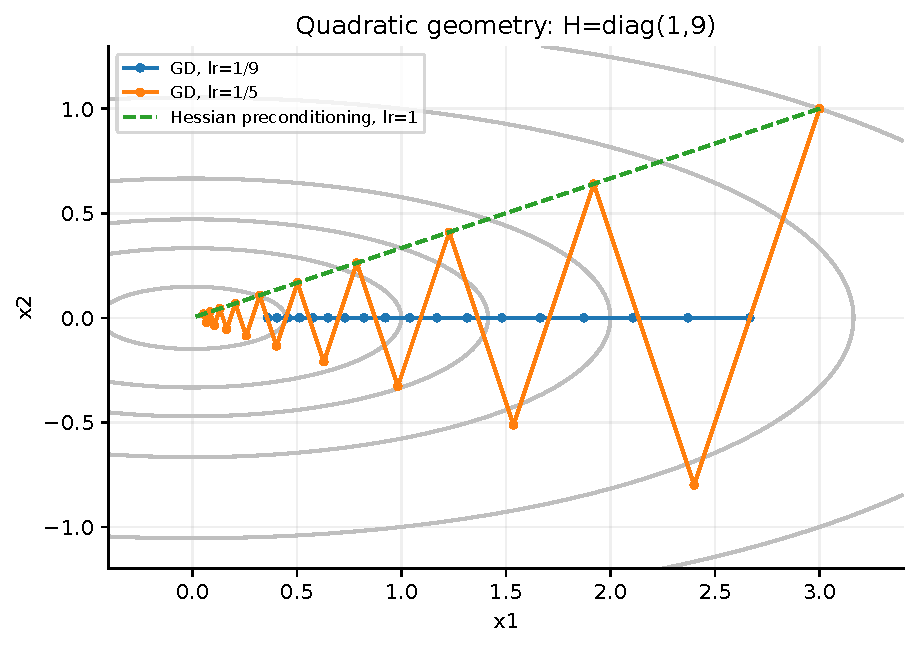
\includegraphics[width=0.85\textwidth]{figures/quadratic_geometry.pdf}
\caption{二次目标 $f(x)-f^*=\tfrac12e^\top He$ 的下降几何，其中 $e=x-x^*$、$H=\diag(1,9)$、$e_0=(3,1)^\top$。步长 $\eta=1/9$ 一步消除高曲率方向的误差，随后沿低曲率方向缓慢前进；$\eta=1/5$ 使两个方向的收缩幅度同为 $4/5$，高曲率坐标交替变号但振幅衰减。使用 Hessian 逆预条件 $P=H^{-1}$ 时，有效 Hessian 为单位阵，单位步长可一步消除该二次模型的误差。}
\label{l1:fig-quadratic-geometry}
\end{figure}

\section{不知道光滑常数时：回溯线搜索}
\label{l1:line-search}

实际问题中，全局 $L$ 可能难以估计，也可能比当前区域的曲率大很多。回溯线搜索利用已计算的梯度，试探一个足够下降的步长。设 $d_t$ 满足 $\inner{\nabla f(x_t)}{d_t}<0$，选择 $c\in(0,1)$、$\beta\in(0,1)$ 和初始试探步长 $\alpha_0>0$。从 $\alpha=\alpha_0$ 开始，若
\begin{equation}
 f(x_t+\alpha d_t)
 \leq f(x_t)+c\alpha\inner{\nabla f(x_t)}{d_t}
 \label{l1:armijo}
\end{equation}
不成立，就令 $\alpha\leftarrow\beta\alpha$ 并重试。接受后设置 $x_{t+1}=x_t+\alpha d_t$。式\eqref{l1:armijo}称为 Armijo 充分下降条件；它比较实际下降与一阶模型预测下降的一定比例\citep{Nocedal2006}。

\begin{proposition}[回溯何时有限终止]
\label{l1:prop-backtracking}
若 $\nabla f(x_t)^\top d_t<0$，且试探线段附近梯度为 $L$-Lipschitz，则任意满足
\[
 0<\alpha\leq
 \frac{-2(1-c)\inner{\nabla f(x_t)}{d_t}}{L\norm{d_t}^2}
\]
的步长都满足 Armijo 条件。因此，几何回溯会有限终止。对 $d_t=-\nabla f(x_t)$，充分条件简化为 $\alpha\leq2(1-c)/L$。
\end{proposition}

\begin{proof}
下降引理给出
\[
 f(x_t+\alpha d_t)
 \leq f(x_t)+\alpha\inner{g_t}{d_t}
       +\frac{L\alpha^2}{2}\norm{d_t}^2.
\]
要求右侧不超过 $f(x_t)+c\alpha\inner{g_t}{d_t}$，整理即得。
\end{proof}

线搜索并非免费：一次梯度更新可能需要多次目标评估。对全批量问题，这常是合理成本；对随机 mini-batch，若每次试探都更换数据，比较的就不再是同一个函数，以上结论不能直接使用。算法理论中的一个“迭代步”与实验中的一次前向、一次反向、一次数据遍历必须区分。

停止准则也要说明能证明什么。在强凸情形，$\norm{\nabla f(x)}\leq\varepsilon$ 给出目标差不超过 $\varepsilon^2/(2\mu)$。一般非凸情形，小梯度只是一阶驻点证据。单独使用“连续两步损失变化很小”不可靠：步长过小也会产生这一现象。实际可联合检查梯度、步长、目标变化和预算，并记录它们各自的量纲。

\section{Newton 法：利用曲率，也检验曲率}
\label{l1:newton}

\subsection{二次局部模型与下降方向}

设 $f$ 二阶可微，$g_t=\nabla f(x_t)$、$H_t=\nabla^2f(x_t)$。Newton 法在当前点使用模型
\[
 m_t(d)=f(x_t)+\inner{g_t}d+\frac12d^\top H_td.
\]
当 $H_t\succ0$ 时，该模型唯一极小点解方程
\begin{equation}
 H_td_t=-g_t,
 \qquad x_{t+1}=x_t+\alpha_td_t.
 \label{l1:newton-step}
\end{equation}
而且 $g_t^\top d_t=-g_t^\top H_t^{-1}g_t<0$，所以非零梯度下它是下降方向。对严格凸二次目标，Hessian 不随位置改变，取 $\alpha_t=1$ 一步到达最优点。

这并不意味着 Newton 法总比梯度下降快。每步需要表示或近似曲率、求解线性系统；在高维学习问题中，这些成本可能显著。更关键的是，远离最优点时二次模型可能不准确，非凸 Hessian 还可能不正定。一个求解了线性方程的向量，不一定是原目标的下降方向。

\begin{example}[步长阻尼与 Hessian 修正处理不同问题]
\label{l1:ex-newton}
先看凸函数 $f(x)=e^x-x$，唯一最优点为0。Newton 方向为
\[
 d(x)=-\frac{e^x-1}{e^x}=e^{-x}-1.
\]
从 $x_0=-2$ 出发，$d_0=e^2-1\approx6.389$。全步长到达 $x_1\approx4.389$，函数值从约2.135增至约76.2。方向本身是下降方向，但走得过远，二次近似失效。

取 Armijo 参数 $c=0.1$、回缩因子 $\beta=1/2$。试探 $\alpha=1$ 失败；$\alpha=1/2$ 时函数值约2.107，仍未达到所要求的充分下降；$\alpha=1/4$ 时到达约 $-0.403$，函数值约1.071，满足条件。这是通过缩短步长来控制模型误差。

再看非凸函数 $h(x)=x^4/4-x^2/2$。在 $x=0.1$，有 $h'(x)=-0.099$、$h''(x)=-0.97$，Newton 方向约为 $-0.1021$，与梯度内积为正。此时方向向局部极大点0移动，任意足够小的正步长都会上升。仅做步长回缩无法把上升方向变成下降方向；必须先修正曲率模型或更换方向。
\end{example}

一种曲率修正是求解
\[
 (H_t+\tau_t I)d_t=-g_t,
 \qquad H_t+\tau_t I\succ0,
\]
再配合线搜索。这里 $\tau_t$ 改变方向，$\alpha_t$ 改变沿该方向走多远。二者有不同职责。还可以使用信赖域，直接限制二次模型的可信区域；其完整理论留作\citet{Nocedal2006}的延伸阅读。

\subsection{选读：局部二次收敛的准确条件}

\begin{theorem}[Newton 法的局部误差界]
\label{l1:thm-newton-local}
设 $\nabla f(x^*)=0$。在以 $x^*$ 为中心的某个凸邻域中，假设
\[
 \nabla^2f(x)\succeq\mu I\quad(\mu>0),\qquad
 \norm{\nabla^2f(x)-\nabla^2f(y)}_2\leq M\norm{x-y}.
\]
若当前点 $x_t$ 位于该邻域，Newton 全步的误差满足
\begin{equation}
 \norm{x_{t+1}-x^*}\leq\frac{M}{2\mu}\norm{x_t-x^*}^2.
 \label{l1:newton-quadratic}
\end{equation}
若初始点足够近，使上述误差界保证后续点始终留在邻域内，则全步 Newton 法局部二次收敛。
\end{theorem}

\begin{proof}
令 $e_t=x_t-x^*$，由梯度的积分表达式，
\[
 g_t=\int_0^1\nabla^2 f(x^*+se_t)e_t\,ds.
\]
因此
\[
 e_{t+1}=H_t^{-1}\int_0^1
 \bigl[H_t-\nabla^2f(x^*+se_t)\bigr]e_t\,ds.
\]
利用 $\norm{H_t^{-1}}_2\leq1/\mu$ 与 Hessian 的 Lipschitz 条件，积分上界为
\[
 \frac1\mu\int_0^1M(1-s)\norm{e_t}^2\,ds
 =\frac{M}{2\mu}\norm{e_t}^2.
\]
例如选取包含于原邻域、半径不超过 $\mu/M$ 的球，就可由误差至少减半保证迭代不离开该球；$M=0$ 时对应局部精确二次模型。
\end{proof}

“二次收敛”是局部误差递推的阶数，不能解释成对任何初始化都只需很少步，也不能忽略求线性系统的数值误差。精确理论为阻尼策略提供目标：远处先保证进展，进入合适区域后再利用全步的快速收敛。

\section{预条件：改变更新所使用的几何}
\label{l1:preconditioning}

选择对称正定矩阵 $P$，考虑
\begin{equation}
 x_{t+1}=x_t-\eta P\nabla f(x_t).
 \label{l1:precondition-update}
\end{equation}
它恰好是下列局部模型的最小点：
\[
 \argmin_z\left\{\inner{\nabla f(x_t)}{z-x_t}
 +\frac1{2\eta}(z-x_t)^\top P^{-1}(z-x_t)\right\}.
\]
换言之，$P^{-1}$ 定义位移的代价。在某个方向给更小的位移代价，就允许该方向更大的更新。这比“每个坐标分别乘一个学习率”的描述更一般，因为 $P$ 可以包含非对角项。

令 $x=P^{1/2}z$，定义 $\widetilde f(z)=f(P^{1/2}z)$，则\eqref{l1:precondition-update}等价于在 $z$ 坐标对 $\widetilde f$ 做普通梯度下降。若原目标为 Hessian $H\succ0$ 的二次函数，新的 Hessian 是
\begin{equation}
 \widetilde H=P^{1/2}HP^{1/2}.
 \label{l1:precondition-hessian}
\end{equation}
有效条件数应根据这个对称矩阵计算。$PH$ 虽不一定对称，但与它相似，具有相同正特征值。取 $P=H^{-1}$ 时，$\widetilde H=I$；对于大型问题，恰恰是精确构造和应用这个逆矩阵的成本促使我们研究对角、块对角或其他结构近似。

\begin{example}[标准化不等于白化]
\label{l1:ex-whitening}
考虑 $H=\begin{pmatrix}1&\rho\\\rho&1\end{pmatrix}$，$0<\rho<1$。两个坐标的尺度已经相同，对角预条件 $P=\diag(H)^{-1}=I$ 完全不改变问题。然而 $H$ 的特征值是 $1+\rho$ 与 $1-\rho$，条件数为 $(1+\rho)/(1-\rho)$；当 $\rho=0.99$ 时条件数为199。

取完整预条件 $P=H^{-1}$ 则有效条件数为1。这说明差异不仅来自边际尺度，也来自坐标之间的相关性。对数据协方差 $\Sigma$，逐坐标标准化得到的是 $D^{-1}\Sigma D^{-1}$，一般只是对角为1的相关矩阵；只有合适的完整白化才把它变为单位阵。后续讨论 BatchNorm、LayerNorm 或自适应优化器时，不能把它们直接称为精确白化。
\end{example}

预条件也揭示了参数化的意义：同一个预测函数若用不同坐标表示，Euclidean 梯度下降通常产生不同的函数更新。只有同时变换更新所用的几何，才可能保留相同轨迹。第五讲会把这一观察推广到网络 Jacobian 与有效训练核。

\section{欠定最小二乘：优化器会选择哪个解}
\label{l1:min-norm}

设 $A\in\R^{n\times d}$ 非零但可能秩亏，考虑
\[
 \min_x\frac12\norm{Ax-b}^2.
\]
当 $\ker A\ne\{0\}$ 时，目标无法区分沿零空间的参数变化。即使训练预测唯一，参数解也可能有无穷多个。此时我们需要回答两个问题：算法是否收敛，以及收敛到哪一个最优解。

\begin{theorem}[梯度下降的最小范数选择]
\label{l1:thm-min-norm}
设 $A\ne0$，固定步长满足 $0<\eta<2/\norm A_2^2$。对最小二乘目标作梯度下降，则
\begin{equation}
 x_t\longrightarrow A^\dagger b+\Pi_{\ker A}x_0,
 \label{l1:min-norm-limit}
\end{equation}
其中 $A^\dagger$ 是 Moore--Penrose 伪逆，$\Pi_{\ker A}$ 是到 $A$ 零空间的正交投影。特别地，从 $x_0=0$ 出发，极限是所有最小二乘解中 Euclidean 范数最小的解。
\end{theorem}

\begin{proof}
取紧致奇异值分解 $A=U_r\Sigma_rV_r^\top$，其中 $r=\rank A$、$\Sigma_r=\diag(\sigma_1,\ldots,\sigma_r)$ 且 $\sigma_i>0$。每次更新 $-\eta A^\top(Ax_t-b)$ 都在 $\operatorname{range}(A^\top)$ 中，所以零空间分量保持为 $\Pi_{\ker A}x_0$。

在第 $i$ 个右奇异向量方向，记 $z_{t,i}=v_i^\top x_t$，则
\[
 z_{t+1,i}=(1-\eta\sigma_i^2)z_{t,i}
              +\eta\sigma_i u_i^\top b.
\]
步长条件保证 $|1-\eta\sigma_i^2|<1$，其极限为 $u_i^\top b/\sigma_i$。合起来就是 $V_r\Sigma_r^{-1}U_r^\top b=A^\dagger b$。

全部最小二乘解为 $A^\dagger b+v$，$v\in\ker A$。两部分正交，故
\[
 \norm{A^\dagger b+v}^2=\norm{A^\dagger b}^2+\norm v^2.
\]
取 $v=0$ 得到唯一最小范数解。该证明不要求 $Ax=b$ 一致。
\end{proof}

该结论是一个完整的隐式偏置例子：目标函数没有写入 $\norm x^2$ 惩罚，但初始化与更新结构仍选出某一类解。这个选择不等于加入固定强度的岭正则；岭回归通常改变拟合结果，而这里极限仍然精确最小化原始最小二乘损失。

\subsection{预条件怎样改变所选解}

对固定 $P\succ0$，从0出发作预条件梯度下降。通过 $x=P^{1/2}z$ 变换，普通梯度下降在 $z$ 空间选择最小 $\norm z$ 的解，所以在 $x$ 空间选择最小 $x^\top P^{-1}x$ 的最小二乘解。若 $A$ 满行秩，则 $Ax=b$ 总可行，且
\begin{equation}
 x_P=P A^\top(AP A^\top)^{-1}b.
 \label{l1:weighted-min-norm}
\end{equation}
相应稳定步长需要满足 $0<\eta<2/\norm{AP^{1/2}}_2^2$。同样的训练误差不保证同样的参数，也不保证在新输入上给出同样的预测。

\begin{example}[同一条插值直线上的两种选择]
\label{l1:ex-min-norm}
设 $A=(1\ \ 2)$、$b=1$。所有插值解满足 $x_1+2x_2=1$。普通梯度下降从0出发，每步都沿向量 $(1,2)^\top$ 移动，因此极限必为该直线与 $\operatorname{span}(1,2)^\top$ 的交点：
\[
 x_I=\frac15(1,2)^\top=(1/5,2/5)^\top.
\]
取 $P=\diag(4,1)$，更新方向改为 $(4,2)^\top$。由\eqref{l1:weighted-min-norm}，
\[
 x_P=\frac18(4,2)^\top=(1/2,1/4)^\top.
\]
二者都使训练损失为0，但 Euclidean 范数平方分别为 $1/5$ 与 $5/16$。第二个解最小化的是 $x_1^2/4+x_2^2$，其值为 $1/8$，低于第一个解的 $17/100$。若测试输入为 $(1,0)$，两者预测分别为 $1/5$ 与 $1/2$。只看训练损失无法判断哪一个预测更合理，还需要关于数据生成过程的假设。
\end{example}

\section{本讲结论如何进入后续课程}
\label{l1:bridge}

本讲建立了三种不同的判断。第一，凸性与强凸性决定哪些驻点可以作为全局最优证书。第二，光滑常数与条件数解释步长限制和收敛速度。第三，参数空间中的几何与初始化决定在多解问题中选择哪个解。它们之间有关联，但不能互相替代：更快的收敛不自动意味着更好的泛化，更小的梯度也不自动意味着解决了非凸全局优化。

第二讲在约束边界处用 KKT 条件替代无约束的 $\nabla f=0$；第三讲研究梯度含随机误差时哪些递推需要增加噪声项；第四讲比较不同几何下的更新；第五讲把 $P$ 与网络 Jacobian 共同纳入函数空间动力学。建议阅读\citet{Boyd2004}的凸函数与无约束最小化章节、\citet{Nesterov2004}的一阶复杂度分析，以及\citet{Nocedal2006}的线搜索与 Newton 方法。课堂证明已经给出本讲所需的主要结论，延伸阅读用于理解更一般的条件和更强的算法。

\section{习题}
\label{l1:exercises}

\begin{exercise}[基本性质与结论边界]
\label{l1:exercise-properties}
分别判断 $f_1(x)=x^4$、$f_2(x)=e^x$、$f_3(x)=x^2/2$ 在整个实线上是否凸、严格凸、强凸、全局光滑，以及是否存在最优点。再说明：把定义域限制为 $[-1,1]$ 后，哪些光滑性结论发生改变？不要用“图像像碗”代替导数或定义证明。
\end{exercise}

\begin{exercise}[梯度下降的谱与稳定性]
\label{l1:exercise-spectrum}
令 $f(x)=\tfrac12(2x_1^2+8x_2^2)$，$x_0=(1,1)^\top$。求保证所有初始化收敛的固定步长区间、最坏方向最优固定步长和相应收缩因子。计算该最优步长下 $x_t$ 与 $f(x_t)$。在边界步长 $\eta=1/4$ 时，为什么目标不一定收敛到0？
\end{exercise}

\begin{exercise}[重新组织收敛证明]
\label{l1:exercise-proof}
对 $L$-光滑凸函数，在 $\eta=1/L$ 下证明
\[
 2\eta(f(x_{t+1})-f^*)\leq
 \norm{x_t-x^*}^2-\norm{x_{t+1}-x^*}^2.
\]
据此证明定理\ref{l1:thm-gd-convex}，并指出若删去凸性，证明的哪一步失效。若只保留光滑性与 $f\geq f_{\inf}$，用一步下降式证明最小梯度平方的 $O(1/T)$ 界。
\end{exercise}

\begin{exercise}[回溯线搜索的手算]
\label{l1:exercise-armijo}
对 $f(x)=5x^2$，从 $x_0=1$ 沿负梯度方向搜索。取 $c=1/4$、$\beta=1/2$、$\alpha_0=1$。求精确的 Armijo 可接受步长区间，并列出回溯第一次接受的步长及新点。说明 $\alpha$ 是沿方向的系数，不能再额外乘一次梯度范数。
\end{exercise}

\begin{exercise}[Newton 法与方向修正]
\label{l1:exercise-newton}
对 $h(x)=x^4/4-x^2/2$，求全部驻点及其类型。在 $x=0.1$ 处，分别计算原始 Newton 方向与使用 $h''(x)+2$ 的修正方向，并验证哪一个是下降方向。讨论为什么“Newton 步长足够小就一定下降”不是正确命题。
\end{exercise}

\begin{exercise}[初始化保留的零空间]
\label{l1:exercise-nullspace}
令 $A=(1\ \ 1)$、$b=1$，初始点为 $x_0=(2,0)^\top$。求普通梯度下降的极限，并比较它与零初始化的极限。再从0出发，取 $P=\diag(1,4)$，求预条件梯度下降的极限与稳定步长区间。解释三个解各自在什么集合、什么距离意义下被选中。
\end{exercise}

\begin{exercise}[选读：正则化极限与早停滤波]
\label{l1:exercise-filters}
设 $A=U_r\Sigma_rV_r^\top$。写出岭回归解 $x_\lambda$ 的奇异向量展开，并证明 $\lambda\downarrow0$ 时它趋向 $A^\dagger b$。再写出零初始化梯度下降的 $x_T$，比较岭回归与有限步迭代对小奇异值方向的权重。说明“都抑制小奇异值方向”为什么不意味着二者对所有谱值存在同一个精确等价参数。
\end{exercise}

\section{习题解答要点}
\label{l1:solutions}

\paragraph{习题\ref{l1:exercise-properties}.}
$x^4$ 凸且严格凸，有唯一最优点0；因 $f''(0)=0$ 而不强凸，因 $f''$ 无界而不全局光滑。$e^x$ 凸且严格凸，无有限最优点；二阶导的下确界为0、上确界无穷，所以既不在实线上强凸，也不全局光滑。$x^2/2$ 是1-强凸、1-光滑，唯一最优点0。在 $[-1,1]$ 上，前两者分别可取光滑常数12和 $e$；$e^x$ 还可取强凸常数 $e^{-1}$，最优点成为边界 $-1$。边界最优点不要求导数为零。

\paragraph{习题\ref{l1:exercise-spectrum}.}
稳定区间为 $0<\eta<1/4$，最优固定步长为 $2/(2+8)=1/5$，误差因子为 $3/5$。因此 $x_t=((3/5)^t,(-3/5)^t)^\top$，$f(x_t)=5(9/25)^t$。当 $\eta=1/4$，第二坐标的因子是 $-1$，非零初始分量永久振荡；它贡献的目标值始终为4。稳定结论必须明确是对全部初始化还是某个特殊初始化。

\paragraph{习题\ref{l1:exercise-proof}.}
将凸性上界 $f(x_t)-f^*\leq g_t^\top(x_t-x^*)$ 与下降引理合并，再展开距离平方，即得题设式。求和后利用函数值单调性得到末次迭代的界。没有凸性时，梯度内积不再控制全局目标差，但仍有
\[
 \frac1T\sum_{t=0}^{T-1}\norm{\nabla f(x_t)}^2
 \leq\frac{2L(f(x_0)-f_{\inf})}{T},
\]
从而最小梯度平方不超过同一上界。它是驻点保证，不是全局最优保证。

\paragraph{习题\ref{l1:exercise-armijo}.}
方向为 $d_0=-10$。条件 $5(1-10\alpha)^2\leq5-25\alpha$ 等价于 $0<\alpha\leq3/20$。回溯依次试探 $1,1/2,1/4,1/8$，在 $1/8$ 接受；新点为 $1-10/8=-1/4$。该点越过最优点，但目标仍充分下降。

\paragraph{习题\ref{l1:exercise-newton}.}
驻点为 $0,\pm1$；0是严格局部极大，$\pm1$ 是全局极小。原始方向 $-(-0.099)/(-0.97)\approx-0.1021$，与梯度内积为正。修正曲率为1.03，方向为 $0.099/1.03\approx0.0961$，与梯度内积为负。只有先获得下降方向，充分小正步长才有下降保证。

\paragraph{习题\ref{l1:exercise-nullspace}.}
$A^\dagger b=(1/2,1/2)^\top$，$x_0$ 的零空间投影为 $(1,-1)^\top$，故第一种极限为 $(3/2,-1/2)^\top$。零初始化的极限是 $(1/2,1/2)^\top$。预条件极限为 $(1/5,4/5)^\top$，因为 $APA^\top=5$，稳定步长为 $0<\eta<2/5$。前两者是在解直线上距离各自初始点最近的 Euclidean 解；第三个是零初始化下最小化 $x_1^2+x_2^2/4$ 的解。

\paragraph{习题\ref{l1:exercise-filters}.}
两种展开分别为
\[
 x_\lambda=\sum_{i=1}^r\frac{\sigma_i}{\sigma_i^2+\lambda}
                 (u_i^\top b)v_i,
\qquad
 x_T=\sum_{i=1}^r
 \frac{1-(1-\eta\sigma_i^2)^T}{\sigma_i}(u_i^\top b)v_i.
\]
在稳定步长下，两者分别令 $\lambda\downarrow0$ 与 $T\to\infty$，都得到伪逆解。若还取 $\eta\leq1/\norm A_2^2$，有限步滤波因子处于 $[0,1]$，便于直接比较小谱方向的抑制。岭回归的滤波形状是有理函数，早停对应迭代多项式；一个标量参数一般不能使它们同时匹配多个不同奇异值。

\chapter{对偶、KKT 与约束优化}
\label{l2:chapter}

\begin{coursebox}{本讲目标与课堂安排}
无约束问题在最优点满足 $\nabla f=0$；加入预算、守恒或安全约束后，最优点常在边界，梯度可以不为零。本讲的核心是用对偶与 Karush--Kuhn--Tucker（KKT）条件描述这种边界最优性，并据此构造可计算的算法。

本讲为三个理论学时。按每学时45分钟，建议安排：对偶与 Slater 条件30分钟，KKT 的条件边界及两个二维例题55分钟，投影与近端25分钟，罚函数与增广 Lagrangian 25分钟。LICQ 必要性证明、完整近端收敛证明和对偶迭代的补充例子为选读。课堂结束时，应能独立列出并核验完整 KKT 条件，解释乘子的符号与尺度，并说明凸问题的最优证书和非凸问题的驻点证据有何不同。
\end{coursebox}

\section{约束改变了最优性的表达}
\label{l2:problem}

本讲采用统一符号
\begin{equation}
 \begin{aligned}
 \min_{x\in\R^d}\quad & f(x),\\
 \text{s.t.}\quad & g_i(x)\leq0,\qquad i=1,\ldots,m,\\
 & h_j(x)=0,\qquad j=1,\ldots,p.
 \end{aligned}
 \label{l2:primal}
\end{equation}
除另行说明外，$f,g_i,h_j$ 均连续可微。可行点满足所有约束，可行集合记为 $C$，原始最优值记为 $p^*$。在点 $x\in C$，满足 $g_i(x)=0$ 的不等式称为活跃约束，其指标集合为 $\mathcal I(x)$。严格满足 $g_i(x)<0$ 的约束在足够小的邻域内不限制位移方向。

例如，$\min_{x\geq0}x$ 的唯一最优点是0，但目标导数是1而不是0。向负方向移动可以减少目标，却违反约束；向正方向移动虽然可行，却增加目标。因此约束最优性要求的是“没有可行下降方向”，而非“所有方向的一阶变化都为零”。

\begin{definition}[本讲采用的凸规划形式]
当 $f$ 与所有 $g_i$ 是凸函数，且等式约束为仿射形式 $h(x)=Ax-b$ 时，称\eqref{l2:primal}为凸规划。它的可行集合是凸集。等式若写成一般非线性凸函数等于0，其零水平集也未必凸，不能只凭“每个函数都凸”就认定整个问题是凸规划。
\end{definition}

约束表示本身也有影响。例如 $x=0$ 与 $x^2\leq0$ 定义同一个集合，但它们在0处的约束梯度分别为1和0。算法和乘子条件需要使用约束函数的导数，所以仅知道可行集合相同，还不足以保证两种表示同样适合数值求解。

\section{Lagrangian 与对偶：先建立下界}
\label{l2:duality}

\subsection{为什么不等式乘子必须非负}

引入不等式乘子 $\lambda\in\R^m$ 与等式乘子 $\nu\in\R^p$，定义 Lagrangian
\begin{equation}
 \mathcal L(x,\lambda,\nu)
 =f(x)+\sum_{i=1}^m\lambda_i g_i(x)
       +\sum_{j=1}^p\nu_jh_j(x).
 \label{l2:lagrangian}
\end{equation}
当 $x$ 可行且 $\lambda\geq0$ 时，$\lambda_i g_i(x)\leq0$，而等式项为0，故 $\mathcal L(x,\lambda,\nu)\leq f(x)$。乘子的符号由这一不等式决定；若把原约束改写为 $g_i(x)\geq0$，就必须相应调整符号约定。等式乘子没有符号限制。

定义对偶函数
\begin{equation}
 q(\lambda,\nu)=\inf_{x\in\R^d}\mathcal L(x,\lambda,\nu),
 \label{l2:dual-function}
\end{equation}
它允许取 $-\infty$。这里对 $x$ 的最小化已经去掉原约束，因为约束信息进入了乘子项。若误把 $\inf_x$ 再限制在原可行集合，会得到另一个对象，通常失去对偶方法的作用。

\begin{proposition}[弱对偶]
\label{l2:prop-weak-duality}
对任意原始可行点 $x$ 和任意 $\lambda\geq0,\nu$，均有
\[
 q(\lambda,\nu)\leq\mathcal L(x,\lambda,\nu)\leq f(x).
\]
因此对偶问题
\begin{equation}
 d^*=\sup_{\lambda\geq0,\nu}q(\lambda,\nu)
 \label{l2:dual-problem}
\end{equation}
满足 $d^*\leq p^*$。这个结论不要求原问题凸。
\end{proposition}

对每个固定 $x$，$\mathcal L$ 关于 $(\lambda,\nu)$ 都是仿射函数。仿射函数族的逐点下确界是凹函数，所以 $q$ 总是凹的，即使原问题非凸。对偶问题是在凸集合 $\lambda\geq0$ 上最大化凹函数；“对偶问题具有凸优化结构”并不意味着原问题的非凸性已经消失，因为可能存在正的对偶间隙 $p^*-d^*$。

\subsection{可计算的最优性证书}

若 $x$ 原始可行、$(\lambda,\nu)$ 对偶可行，且 $q$ 有限，则
\begin{equation}
 0\leq f(x)-p^*\leq f(x)-q(\lambda,\nu).
 \label{l2:gap-certificate}
\end{equation}
因此，一个可行解与一个下界可以共同构成最优性证书。优化软件报告的 primal--dual gap 正是利用这一思想。若当前 $x$ 不可行，$f(x)$ 不能直接作为可行最优值的上界，此时即使数值上的“gap”很小，也不能使用\eqref{l2:gap-certificate}。

对偶值与乘子并不是随意添加的辅助变量。它们分别提供“目前至少不可能比什么值更好”和“哪些约束正在阻止目标进一步下降”的信息。后者会在影子价格分析中变得具体。

\section{强对偶与 Slater 条件}
\label{l2:slater}

弱对偶始终成立，强对偶 $d^*=p^*$ 则需要额外条件。本讲使用一个足够常用、假设清楚的版本\citep{Boyd2004}。

\begin{theorem}[Slater 条件下的强对偶]
\label{l2:thm-slater}
设 $f,g_1,\ldots,g_m$ 在整个 $\R^d$ 上有限、凸且可微，$h(x)=Ax-b$。假设最优值有限，并存在严格可行点 $\bar x$ 满足
\[
 A\bar x=b,\qquad g_i(\bar x)<0\quad(i=1,\ldots,m).
\]
则 $d^*=p^*$，且存在达到对偶最优值的乘子 $(\lambda^*,\nu^*)$。若原始最优值也在某个 $x^*$ 处取到，则该点存在满足完整 KKT 条件的乘子。
\end{theorem}

这里的严格可行只针对不等式；等式必须精确满足，不能要求“严格等于”。当模型具有受限定义域时，还要使用相对内部来表达合适的 Slater 条件。本讲把函数设为在整个 $\R^d$ 上有限，是为了避免在初次学习时把域的边界和不等式约束混在一起。

Slater 是充分条件，不是必要条件。某个问题不满足它，不能立即宣布存在对偶间隙；可能仍然强对偶，也可能最优乘子不取到。应分别检查“最优值是否相等”和“最优解或乘子是否存在”。下一节的退化约束例子会同时说明这些区别。

\paragraph{选读：强对偶证明的几何入口.}
把约束右端放宽为 $g(x)\leq u$、$h(x)=v$，考察集合
\[
 \mathcal A=\{(u,v,t):\ \exists x,\quad
       g(x)\leq u,\ h(x)=v,\ f(x)\leq t\}.
\]
目标与不等式的凸性、等式的仿射性使 $\mathcal A$ 为凸集，分离超平面可以为最优值提供线性下界。若等式存在冗余，应先删除冗余等式，或在可达扰动的相对仿射空间中使用分离定理；否则可能存在仅来自不可达等式扰动方向的退化法向量。作此处理后，严格可行排除相关的不正常分离情形，使目标系数能够规范化为1。将规范化后的约束系数写成 $\lambda\geq0,\nu$，便得到达到 $p^*$ 的 Lagrangian 下界。这是 Slater 条件与乘子存在之间的联系；完整分离论证可阅读\citet{Boyd2004}的对偶章节。

\section{KKT 条件：四组方程和三种适用范围}
\label{l2:kkt}

\subsection{完整条件不能只剩“梯度为零”}

对候选点 $(x^*,\lambda^*,\nu^*)$，完整 KKT 条件是
\begin{align}
 g_i(x^*)&\leq0,\quad h_j(x^*)=0
 &&\text{（原始可行性）},\label{l2:kkt-primal}\\
 \lambda_i^*&\geq0
 &&\text{（对偶可行性）},\label{l2:kkt-dual}\\
 \lambda_i^*g_i(x^*)&=0
 &&\text{（互补松弛）},\label{l2:kkt-complementarity}\\
 \nabla f(x^*)+\sum_i\lambda_i^*\nabla g_i(x^*)
       +\sum_j\nu_j^*\nabla h_j(x^*)&=0
 &&\text{（驻点条件）}.
 \label{l2:kkt-stationarity}
\end{align}
互补松弛的含义是：严格松弛约束的乘子必须为0；乘子为正的约束必须活跃。反向命题不成立，活跃约束的乘子也可以为0。列出驻点方程而忘掉乘子的非负性，会把不可接受的候选点混入解集。

\begin{theorem}[凸问题中 KKT 的充分性与必要性]
\label{l2:thm-convex-kkt}
设 $f,g_i$ 凸且可微，$h$ 仿射。
\begin{enumerate}
 \item 只要某个三元组满足全部 KKT 条件，$x^*$ 就是全局最优点，乘子为对偶最优解，且对偶间隙为0。此充分性不需要额外的 Slater 条件。
 \item 若最优点存在，且满足定理\ref{l2:thm-slater}的 Slater 假设，则每个原始最优点均存在使 KKT 成立的乘子。
\end{enumerate}
\end{theorem}

\begin{proof}
先证充分性。因为 $\lambda^*\geq0$，$x\mapsto\mathcal L(x,\lambda^*,\nu^*)$ 是凸函数。驻点条件使 $x^*$ 为它的全局极小点，互补松弛和可行性给出 $\mathcal L(x^*,\lambda^*,\nu^*)=f(x^*)$。对任意可行 $x$，
\[
 f(x)\geq\mathcal L(x,\lambda^*,\nu^*)
 \geq\mathcal L(x^*,\lambda^*,\nu^*)=f(x^*).
\]
同时 $q(\lambda^*,\nu^*)=f(x^*)$，所以乘子也达到对偶最优值。

再证必要性。Slater 保证存在对偶最优乘子，且 $q(\lambda^*,\nu^*)=f(x^*)$。弱对偶中的两个不等式此时必须都取等号：$x^*$ 最小化 Lagrangian，所以其梯度为0；又因为每个 $\lambda_i^*g_i(x^*)\leq0$ 而总和为0，每一项都必须为0，得到互补松弛。
\end{proof}

\subsection{非凸问题中的必要性：约束资格条件}

\begin{definition}[线性无关约束资格条件 LICQ]
在可行点 $x^*$，如果向量集合
\[
 \{\nabla g_i(x^*):i\in\mathcal I(x^*)\}
 \ \cup\ \{\nabla h_j(x^*):j=1,\ldots,p\}
\]
线性无关，则称 LICQ 在该点成立。只把活跃不等式放入这个集合。
\end{definition}

\begin{theorem}[非凸局部最优点的 KKT 必要条件]
\label{l2:thm-licq}
设目标与约束在 $x^*$ 邻域连续可微，$x^*$ 是局部极小点，且 LICQ 成立。则存在满足 KKT 条件的乘子，且这些乘子唯一。该定理不要求凸性，也不保证任何 KKT 点是局部或全局极小点。
\end{theorem}

\paragraph{选读：必要性证明.}
考虑线性化可行方向 $d$，满足 $\nabla h_j(x^*)^\top d=0$、$\nabla g_i(x^*)^\top d\leq0$ 对所有活跃 $i$ 成立。若同时 $\nabla f(x^*)^\top d<0$，LICQ 允许找到方向 $d_0$，使所有等式的一阶变化为0、所有活跃不等式的一阶变化为 $-1$。对足够小的 $\epsilon>0$，$d+\epsilon d_0$ 仍为下降方向，而且严格进入所有活跃不等式内部。等式 Jacobian 满秩，隐函数定理给出具有这一切向量的等式可行曲线；足够短的一段曲线便是可行下降路径，与局部最优矛盾。

因此不存在上述线性化下降方向。有限维 Farkas 择一定理表明，这等价于 $-\nabla f(x^*)$ 属于活跃约束梯度的非负锥与等式梯度线性空间之和。这恰好给出驻点条件中的非负 $\lambda$ 与自由 $\nu$；非活跃乘子置0后得到互补松弛。最后，若有两组乘子，减去两条驻点方程，LICQ 强制它们完全相同。相关约束资格与必要条件可参见\citet{Nocedal2006}。

\begin{example}[LICQ 失败：有最优解但不存在 KKT 乘子]
\label{l2:ex-licq-failure}
考虑凸问题
\[
 \min_x x\qquad\text{s.t.}\qquad x^2\leq0.
\]
唯一可行点是 $x^*=0$，因此它当然全局最优。可是 $g'(0)=0$，LICQ 失败，驻点方程要求 $1+\lambda\cdot0=0$，没有任何有限乘子能够满足。

这个例子还可以完整算出对偶。当 $\lambda>0$，
\[
 q(\lambda)=\inf_x(x+\lambda x^2)=-\frac1{4\lambda};
\]
当 $\lambda=0$，$q(0)=-\infty$。故 $d^*=\sup_{\lambda\geq0}q(\lambda)=0=p^*$，但对偶最优值只在 $\lambda\to\infty$ 时逼近，没有有限最优乘子。这里强对偶成立，Slater 不成立，KKT 乘子不存在，三个事实并不矛盾。

若把同一集合写为等式 $h(x)=x=0$，驻点条件成为 $1+\nu=0$，可取 $\nu=-1$。改变约束表示修复了导数退化，而没有改变可行点。
\end{example}

LICQ 失败并不意味着 KKT 一定失败。例如 $\min_x\tfrac12(x-1)^2$，约束为 $x\leq0$ 与 $2x\leq0$。在最优点0，两条活跃梯度相关，但严格可行点 $x=-1$ 存在。KKT 乘子满足 $\lambda_1+2\lambda_2=1$、$\lambda\geq0$，有无穷多组。这说明 Slater 关注凸对偶与乘子存在，LICQ 还排除了活跃约束的冗余并保证乘子唯一；不能把二者当作同一个条件。

\subsection{KKT 点为什么未必是非凸极小点}

考虑 $\min_{-1\leq x\leq1}-x^2$。在 $x=0$，两条不等式均不活跃，取乘子全为0便满足 KKT；但该点是严格局部极大点，真正的最优点为 $\pm1$。因此，在非凸问题中求解 KKT 方程通常只是在找候选点。

二阶判断还必须沿可行方向进行。对于仅含等式的二阶可微问题，在 LICQ 与 KKT 成立时，局部极小点要求 Lagrangian Hessian 在切空间 $\{d:J_h(x^*)d=0\}$ 上半正定；若在所有非零切向量上正定，则可获得严格局部极小的充分条件。带不等式时，应进一步使用临界锥，不能直接要求或检查整个空间上的 Hessian 正定来替代约束二阶分析。

\begin{coursebox}{使用 KKT 前先辨认问题属于哪一类}
凸目标、凸不等式、仿射等式：满足 KKT 就是全局最优证书；要保证最优点一定有乘子，可以检查 Slater。一般非凸问题：局部最优点在 LICQ 等约束资格下必须满足 KKT；找到 KKT 点之后仍需二阶条件、问题结构或其他证据判断其性质。退化约束：最优点可能没有有限 KKT 乘子，应先检查约束表示和资格条件。
\end{coursebox}

\section{完整例题：二维二次规划与影子价格}
\label{l2:worked}

\subsection{预算约束下的投影问题}

\begin{example}[从活跃集到原始--对偶证书]
\label{l2:ex-budget}
给定预算 $b>0$，求解
\begin{equation}
 \min_{x_1,x_2}\ \frac12\bigl[(x_1-2)^2+(x_2-1)^2\bigr],
 \quad x_1+x_2\leq b,\quad x_1\geq0,\ x_2\geq0.
 \label{l2:budget-problem}
\end{equation}
这是把点 $(2,1)$ 投影到非负预算集合。令预算乘子为 $\lambda\geq0$，非负约束 $-x_i\leq0$ 的乘子为 $\alpha_i\geq0$。Lagrangian 为
\[
 \mathcal L=\frac12\norm{x-(2,1)^\top}^2
        +\lambda(x_1+x_2-b)-\alpha_1x_1-\alpha_2x_2.
\]
驻点条件是
\[
 x_1-2+\lambda-\alpha_1=0,\qquad
 x_2-1+\lambda-\alpha_2=0.
\]
还需同时满足三条可行性、三个非负乘子条件，以及
\[
 \lambda(x_1+x_2-b)=0,\qquad\alpha_1x_1=\alpha_2x_2=0.
\]

先取 $b=2$。无约束解 $(2,1)$ 不可行，因此尝试预算活跃、两坐标均为正。互补松弛给出 $\alpha_1=\alpha_2=0$，于是 $x_1=2-\lambda$、$x_2=1-\lambda$。结合 $x_1+x_2=2$，得
\[
 x^*=(3/2,1/2)^\top,\qquad\lambda^*=1/2,
 \qquad\alpha^*=0.
\]
解出的坐标确实为正，乘子也非负，所以所猜活跃集自洽。问题凸，因此这已经证明全局最优；强凸目标进一步保证该原始解唯一。

还可以计算独立的对偶下界。令 $c=(\lambda-\alpha_1,\lambda-\alpha_2)^\top$，对 $x$ 无约束最小化得到
\[
 q(\lambda,\alpha)
 =3\lambda-2\alpha_1-\alpha_2
 -\frac12\bigl[(\lambda-\alpha_1)^2+(\lambda-\alpha_2)^2\bigr]
 -\lambda b.
\]
在上述乘子处 $q=1/4$；原始目标也是 $1/4$，所以 gap 精确为0。

现在让 $b$ 变化。对 $0<b\leq1$，第二坐标被压到0，得到 $x^*=(b,0)^\top$、$\lambda^*=2-b$、$\alpha_2^*=1-b$、$\alpha_1^*=0$。对 $1\leq b\leq3$，两个坐标非负，解为 $((b+1)/2,(b-1)/2)^\top$，预算乘子为 $(3-b)/2$。当 $b\geq3$，无约束解已经可行，所有乘子可以取0。最优值为
\begin{equation}
 p(b)=
 \begin{cases}
 \tfrac12[(b-2)^2+1],&0<b\leq1,\\
 (3-b)^2/4,&1\leq b\leq3,\\
 0,&b\geq3.
 \end{cases}
 \label{l2:budget-value}
\end{equation}
各区间都满足 $p'(b)=-\lambda^*(b)$。例如在 $b=2$，多增加很小的预算 $\delta b$，最优目标约下降 $\delta b/2$。在 $b=3$，预算约束活跃但乘子为0，这是“活跃不一定正乘子”的具体例子。
\end{example}

\begin{figure}[htbp]
\centering
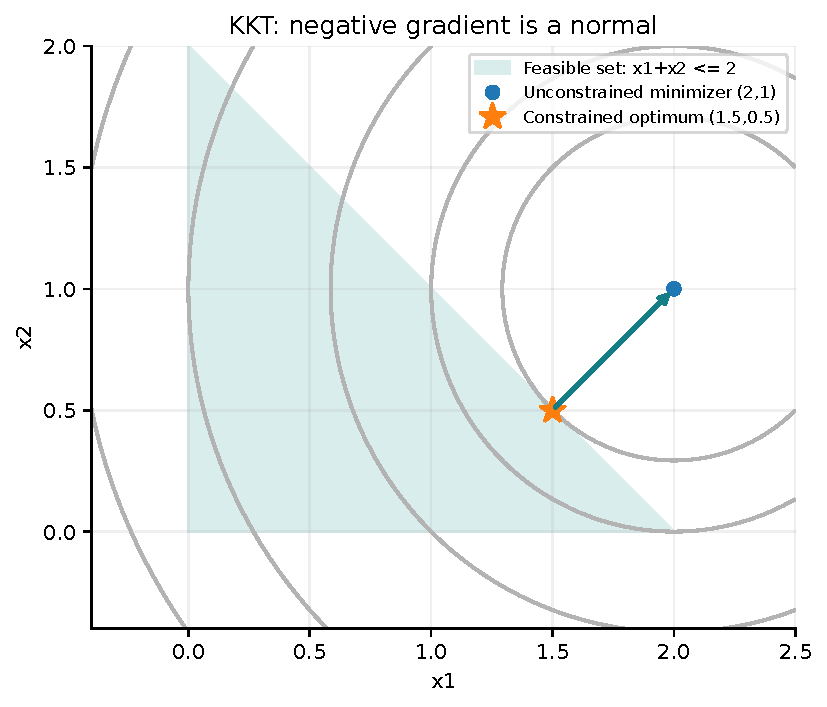
\includegraphics[width=0.85\textwidth]{figures/kkt_geometry.pdf}
\caption{预算为 $b=2$ 时，将 $z=(2,1)^\top$ 投影到可行集 $\{x\geq0:x_1+x_2\leq2\}$。最优点为 $x^*=(1.5,0.5)^\top$，预算约束活跃而两个非负约束均不活跃。预算边界的外法向量为 $(1,1)^\top$，乘子 $\lambda^*=0.5$ 使 $x^*-z+\lambda^*(1,1)^\top=0$；投影位移与活跃边界正交。目标值与对偶下界均为 $1/4$，给出零间隙的全局最优证书。}
\label{l2:fig-kkt-geometry}
\end{figure}

这个例子展示了一种可复用的解题顺序：先写标准符号，再猜活跃集，用互补松弛删去无关乘子，解驻点与活跃约束方程，最后回代核验全部不等式。若核验失败，改变活跃集；不能只保留代数方程的解。

\subsection{球约束也是二次约束：乘子的单位必须明确}

\begin{example}[二次目标与二次约束的完整 KKT 解]
\label{l2:ex-ball}
求解
\[
 \min_{x\in\R^2}\frac12\norm{x-z}^2,
 \qquad \norm x^2\leq4,\qquad z=(3,4)^\top.
\]
目标强凸，约束凸，严格可行点为0。由于 $\norm z=5>2$，无约束解不可行，最优点位于球面。写出
\[
 \mathcal L(x,\lambda)=\frac12\norm{x-z}^2
                         +\lambda(\norm x^2-4).
\]
驻点与互补松弛为
\[
 (1+2\lambda)x=z,
 \qquad \lambda(\norm x^2-4)=0.
\]
若 $\lambda=0$，则 $x=z$ 不可行，故 $\lambda>0$，且 $\norm x=2$。由 $5/(1+2\lambda)=2$ 得
\[
 \lambda^*=\frac34,\qquad x^*=\frac25z=(6/5,8/5)^\top.
\]
该点满足原始可行、对偶可行、互补与驻点四组条件，故为唯一全局最优解，最优值为 $\tfrac12(5-2)^2=9/2$。

进一步无约束最小化 Lagrangian，得到
\[
 q(\lambda)=\frac{25}{2}-\frac{25}{2(1+2\lambda)}-4\lambda,
 \qquad\lambda\geq0.
\]
代入 $3/4$ 得 $q=9/2$，再次核对零对偶间隙。

若把右端记为 $s=R^2$，则在 $0<s<25$，最优值是 $v(s)=\tfrac12(5-\sqrt s)^2$，有 $v'(4)=-3/4=-\lambda^*$。若直接把半径 $R$ 作为资源，则 $d v(R^2)/dR=R-5$，在 $R=2$ 处为 $-3$。二者相差链式法则因子 $2R$。乘子是相对于所写约束右端的价格，不能忽略单位直接比较不同约束的乘子大小。
\end{example}

\subsection{一般的灵敏度不等式}

定义扰动后的最优值
\[
 p(u,v)=\inf\{f(x):g_i(x)\leq u_i,\ h_j(x)=v_j\}.
\]
假设基准问题的最优值 $p(0,0)\in\R$，在 $(u,v)=(0,0)$ 处强对偶，且存在有限的最优乘子 $(\lambda^*,\nu^*)$。对任意扰动可行点，利用基准 Lagrangian 有
\[
 f(x)\geq q(\lambda^*,\nu^*)
                -\lambda^{*\top}u-\nu^{*\top}v.
\]
取下确界得
\begin{equation}
 p(u,v)\geq p(0,0)-\lambda^{*\top}u-\nu^{*\top}v.
 \label{l2:sensitivity-bound}
\end{equation}
在凸问题中，这表示 $(-\lambda^*,-\nu^*)$ 是值函数在原点的一个次梯度。若值函数可微，则
\[
 \nabla_u p(0,0)=-\lambda^*,\qquad
 \nabla_v p(0,0)=-\nu^*.
\]
若不可微，就应保留次梯度或单侧变化的描述，不应声称总存在唯一导数。约束右端放宽通常使最优值不增加，与 $-\lambda_i^*\leq0$ 的符号一致。

\section{把约束最优性变成更新：投影梯度}
\label{l2:projection}

当可行集合 $C$ 非空、闭且凸时，定义 Euclidean 投影
\begin{equation}
 \Pi_C(z)=\argmin_{u\in C}\frac12\norm{u-z}^2.
 \label{l2:projection-definition}
\end{equation}
闭性保证最小值取到，二次目标的强凸性保证唯一性。前面的两个二维例子就是投影问题。对于盒约束，投影是逐坐标截断；对于 Euclidean 球，球外点沿径向缩短；对于一般集合，投影本身可能需要解一个优化问题。

\begin{proposition}[投影的变分不等式]
\label{l2:prop-projection}
令 $p=\Pi_C(z)$，则
\begin{equation}
 \inner{z-p}{u-p}\leq0\qquad\text{对所有 }u\in C.
 \label{l2:projection-vi}
\end{equation}
反过来，满足该不等式的可行点必为投影。投影还满足 $\norm{\Pi_C(z)-\Pi_C(w)}\leq\norm{z-w}$。
\end{proposition}

\begin{proof}
投影目标关于 $u$ 的梯度为 $u-z$，凸约束上的一阶最优性恰为\eqref{l2:projection-vi}；也可沿可行线段求单侧导数直接得到。分别对 $(z,p)$ 和 $(w,q)$ 使用该不等式，选另一个投影点为比较点，相加得到
\[
 \norm{p-q}^2\leq\inner{p-q}{z-w}
 \leq\norm{p-q}\norm{z-w},
\]
由此得非扩张性。
\end{proof}

投影梯度更新为
\begin{equation}
 x_{t+1}=\Pi_C\bigl(x_t-\eta\nabla f(x_t)\bigr).
 \label{l2:projected-gd}
\end{equation}
先做局部下降，再把候选点投回可行集合。它不是任意“修补”参数：投影恰好解出带可行约束的二次局部模型。

定义梯度映射
\begin{equation}
 G_\eta(x)=\frac1\eta\left[x-\Pi_C(x-\eta\nabla f(x))\right].
 \label{l2:gradient-mapping}
\end{equation}
对可行点 $x$，$G_\eta(x)=0$ 等价于 $\inner{\nabla f(x)}{u-x}\geq0$ 对所有 $u\in C$ 成立。若 $f$ 凸，它等价于全局最优；若 $f$ 非凸，它只给出约束一阶驻点条件。此时应检查 $\norm{G_\eta(x)}$，而非强行要求原始梯度趋向0。

\begin{theorem}[投影梯度的凸收敛界]
\label{l2:thm-projected-rate}
设 $C$ 非空、闭且凸，$f$ 在包含 $C$ 的区域上凸且 $L$-光滑，最优点 $x^*\in C$ 存在。由 $x_0\in C$ 出发，取 $0<\eta\leq1/L$，则
\[
 f(x_T)-f(x^*)\leq\frac{\norm{x_0-x^*}^2}{2\eta T}.
\]
\end{theorem}

\begin{proof}
投影最优性给出，对任意 $u\in C$，
\[
 \inner{\nabla f(x_t)}{x_{t+1}-u}
 \leq\frac1\eta\inner{x_t-x_{t+1}}{x_{t+1}-u}.
\]
结合凸性与下降引理，再使用三点距离恒等式，得到
\begin{align}
 f(x_{t+1})-f(u)
 &\leq\frac{\norm{x_t-u}^2-\norm{x_{t+1}-u}^2}{2\eta}
 -\left(\frac1{2\eta}-\frac L2\right)\norm{x_{t+1}-x_t}^2.
 \label{l2:three-point}
\end{align}
令 $u=x_t$ 可得函数值单调不增；令 $u=x^*$ 后求和，便与第一讲一样得到末次迭代的界。
\end{proof}

\section{近端梯度：把投影推广到非光滑正则项}
\label{l2:proximal}

考虑复合目标 $F(x)=f(x)+r(x)$，其中 $f$ 可微，$r$ 为适当、闭、凸函数，可以取 $+\infty$ 以表示禁止某些点。适当指 $r$ 不恒为 $+\infty$ 且从不取 $-\infty$。定义近端算子
\begin{equation}
 \operatorname{prox}_{\eta r}(z)
 =\argmin_u\left\{r(u)+\frac1{2\eta}\norm{u-z}^2\right\}.
 \label{l2:prox-definition}
\end{equation}
在上述条件下，对任意 $z$ 与 $\eta>0$，该解存在且唯一。令 $r=I_C$ 为集合的指示函数：可行时为0，否则为 $+\infty$，就得到 $\operatorname{prox}_{\eta I_C}=\Pi_C$。

近端梯度采取
\begin{equation}
 x_{t+1}=\operatorname{prox}_{\eta r}
                    \bigl(x_t-\eta\nabla f(x_t)\bigr).
 \label{l2:proximal-gradient}
\end{equation}
它线性化光滑部分 $f$，同时保留 $r$ 的完整结构。若把不可微的 $r$ 也随意当作普通梯度处理，就丢失了这个可精确求解的局部模型。

\begin{definition}[凸函数的次梯度]
向量 $v$ 是 $r$ 在 $x$ 的次梯度，如果 $r(u)\geq r(x)+v^\top(u-x)$ 对所有 $u$ 成立。全部次梯度的集合记为 $\partial r(x)$。例如 $\partial|x|=\{1\}$ 当 $x>0$，$\{-1\}$ 当 $x<0$，在0处则为区间 $[-1,1]$。
\end{definition}

近端子问题的一阶最优性是
\begin{equation}
 0\in\partial r(x_{t+1})+\nabla f(x_t)
                         +\frac{x_{t+1}-x_t}{\eta}.
 \label{l2:prox-optimality}
\end{equation}
所以迭代不动点满足 $0\in\nabla f(x)+\partial r(x)$。当 $f$ 也凸时，这是复合目标的全局最优条件；当 $f$ 非凸时，只能称为复合一阶驻点条件。

\begin{example}[软阈值与稀疏更新]
\label{l2:ex-soft-threshold}
取 $r(x)=\tau\norm{x}_1$，近端子问题按坐标分离。在单个坐标上求
\[
 \min_u\ \tau|u|+\frac1{2\eta}(u-z)^2.
\]
若 $u>0$，驻点条件给 $u=z-\eta\tau$，只有 $z>\eta\tau$ 时自洽；若 $u<0$，得到 $u=z+\eta\tau$，要求 $z<-\eta\tau$；若 $u=0$，条件是 $z\in\eta\tau[-1,1]$。因此
\[
 \operatorname{prox}_{\eta\tau\norm{\cdot}_1}(z)_i
 =\operatorname{sign}(z_i)\max\{|z_i|-\eta\tau,0\}.
\]
例如 $z=(1.2,-0.3,0.1)^\top$、$\eta\tau=0.2$，输出为 $(1.0,-0.1,0)^\top$。这产生精确的零坐标；普通小步更新通常只会把坐标推近零。

作为比较，若 $r(x)=\tfrac\tau2\norm x^2$，近端算子为 $z/(1+\eta\tau)$，它连续缩放所有坐标，不产生同样的阈值区间。正则项的几何结构决定近端更新的形状。
\end{example}

\paragraph{选读：近端梯度的速率.}
若 $f$ 凸且 $L$-光滑，$r$ 适当、闭、凸，$x_0$ 位于 $r$ 的有效域，最优点存在，则对 $0<\eta\leq1/L$，
\[
 F(x_T)-F(x^*)\leq\frac{\norm{x_0-x^*}^2}{2\eta T}.
\]
\begin{proof}
由近端最优性条件，向量
\[
 v_{t+1}=\frac{x_t-x_{t+1}}\eta-\nabla f(x_t)
 \quad\text{属于}\quad\partial r(x_{t+1}).
\]
对任意 $u\in\operatorname{dom}r$，次梯度不等式给出
\[
 r(x_{t+1})-r(u)\leq\inner{v_{t+1}}{x_{t+1}-u}.
\]
另一方面，在 $x_t$ 处分别使用 $f$ 的凸性下界与光滑性上界，得到
\[
 f(x_{t+1})-f(u)
 \leq\inner{\nabla f(x_t)}{x_{t+1}-u}
       +\frac L2\norm{x_{t+1}-x_t}^2.
\]
两式相加后，梯度内积相消，故
\begin{align*}
 F(x_{t+1})-F(u)
 &\leq\frac1\eta\inner{x_t-x_{t+1}}{x_{t+1}-u}
       +\frac L2\norm{x_{t+1}-x_t}^2\\
 &=\frac{\norm{x_t-u}^2-\norm{x_{t+1}-u}^2}{2\eta}
   -\left(\frac1{2\eta}-\frac L2\right)
       \norm{x_{t+1}-x_t}^2.
\end{align*}
令 $u=x_t$ 得到 $F(x_{t+1})\leq F(x_t)$；令 $u=x^*$，利用
$\eta\leq1/L$ 丢弃最后的非正项，再对 $t=0,\ldots,T-1$ 求和，便有
\[
 T\bigl(F(x_T)-F(x^*)\bigr)
 \leq\sum_{t=0}^{T-1}\bigl(F(x_{t+1})-F(x^*)\bigr)
 \leq\frac{\norm{x_0-x^*}^2}{2\eta}.
\]
除以 $T$ 即得结论。证明与投影梯度使用同一个三点不等式结构，区别在于用次梯度条件处理完整的非光滑项。
\end{proof}

\section{罚函数与增广 Lagrangian：可行性如何恢复}
\label{l2:penalty}

\subsection{二次罚函数与有限惩罚的偏差}

另一种思路是把违反约束的程度放入目标。对等式 $h(x)=0$ 与不等式 $g(x)\leq0$，二次罚函数为
\begin{equation}
 \Phi_\rho(x)=f(x)+\frac\rho2\norm{h(x)}^2
                    +\frac\rho2\norm{[g(x)]_+}^2,
 \qquad\rho>0,
 \label{l2:quadratic-penalty}
\end{equation}
其中 $[g]_+$ 逐分量取 $\max(g_i,0)$。有限 $\rho$ 通常允许以小量不可行换取目标改善，因此最小化罚函数不等于已经满足原约束。

在较强的理想条件下可以证明可行性恢复：若 $f$ 全局有下界 $f_{\inf}$、存在可行点 $\bar x$，且 $x_\rho$ 是 $\Phi_\rho$ 的全局最小点，则
\[
 \frac\rho2\left(\norm{h(x_\rho)}^2+
                       \norm{[g(x_\rho)]_+}^2\right)
 \leq f(\bar x)-f_{\inf}.
\]
所以违反量至多为 $O(\rho^{-1/2})$。若还有有界子序列与连续性，其聚点可行；利用 $\Phi_\rho(x_\rho)\leq f(x)$ 对每个可行 $x$ 成立，可进一步证明聚点全局最优。这里的“全局求解罚函数”和“存在聚点”都是实质假设，不能直接用于任意非凸局部求解器。

\begin{example}[罚参数越大，子问题可能越病态]
\label{l2:ex-penalty-al}
考虑
\[
 \min_{x_1,x_2}\frac12\bigl[(x_1-2)^2+x_2^2\bigr],
 \qquad x_1=1.
\]
原问题解是 $(1,0)^\top$。对等式 $h(x)=x_1-1$，KKT 乘子为 $\nu^*=1$，因为驻点条件第一维为 $x_1-2+\nu=0$。

二次罚函数的极小点满足
\[
 x_{1,\rho}=\frac{2+\rho}{1+\rho}
           =1+\frac1{1+\rho},\qquad x_{2,\rho}=0.
\]
每个有限 $\rho$ 都有非零可行性误差。其 Hessian 为 $\diag(1+\rho,1)$，条件数为 $1+\rho$。因此提高可行精度的同时，一阶法求解罚子问题也可能变慢。该例不是说所有罚函数必然难解，而是展示“大罚参数”与“好条件数”之间的具体冲突。
\end{example}

\subsection{乘子更新避免只靠无限增大罚参数}

对等式约束定义增广 Lagrangian
\begin{equation}
 \mathcal L_\rho(x,\nu)=f(x)+\nu^\top h(x)
                                  +\frac\rho2\norm{h(x)}^2.
 \label{l2:augmented-lagrangian}
\end{equation}
一种理想化的乘子法是
\begin{align}
 x_{k+1}&\in\argmin_x\mathcal L_\rho(x,\nu_k),\label{l2:al-primal}\\
 \nu_{k+1}&=\nu_k+\rho h(x_{k+1}).\label{l2:al-dual}
\end{align}
罚项提供局部约束曲率，乘子累积可行性残差。与纯罚函数相比，方法不需要仅靠让 $\rho\to\infty$ 才表达正确的约束力。不过一般收敛性仍取决于凸性、子问题求解精度以及其他条件；式子本身不是全局收敛证明。

对例\ref{l2:ex-penalty-al}，可精确计算
\[
 x_{1,k+1}=\frac{2+\rho-\nu_k}{1+\rho},\qquad x_{2,k+1}=0,
\]
从而
\[
 \nu_{k+1}=\frac{\nu_k+\rho}{1+\rho},
 \qquad\nu_{k+1}-1=\frac{\nu_k-1}{1+\rho}.
\]
任意固定 $\rho>0$ 都给出这个例子的线性收敛。取 $\rho=1$、$\nu_0=0$，依次得到 $x_1$ 坐标 $1.5,1.25,1.125,\ldots$，乘子为 $0.5,0.75,0.875,\ldots$，而每个子问题的条件数始终为2。这一完整计算解释了乘子更新的作用，超出了“给损失再加一项”的直觉。

对不等式，可以引入非负松弛变量或采用相应的投影乘子与增广项；不能把等式公式中的自由乘子直接照搬而忘记非负约束。具体算法应明确其 Lagrangian 形式、更新顺序以及内层求解精度。

\subsection{选读：一个能收敛的对偶迭代与一个会发散的同步迭代}

对 $\min_x\tfrac12x^2$、约束 $x=1$，普通 Lagrangian 为 $\tfrac12x^2+\nu(x-1)$。固定 $\nu$ 的精确极小点是 $x(\nu)=-\nu$，故
\[
 q(\nu)=-\tfrac12\nu^2-\nu,\qquad q'(\nu)=-\nu-1.
\]
对偶梯度上升 $\nu_{k+1}=\nu_k+\alpha q'(\nu_k)$ 满足
\[
 \nu_{k+1}+1=(1-\alpha)(\nu_k+1).
\]
于是 $0<\alpha<2$ 时，$\nu_k\to-1$、$x(\nu_k)\to1$。这里每次上升使用的是已经对原变量精确最小化后的对偶函数。

直接同时对原变量下降、对乘子上升，是另一种算法。最简单的 Lagrangian $\mathcal L(x,\nu)=x\nu$ 对应目标0与等式 $x=0$。同步更新为
\[
 \begin{pmatrix}x_{k+1}\\\nu_{k+1}\end{pmatrix}
 =\begin{pmatrix}1&-\eta\\\eta&1\end{pmatrix}
  \begin{pmatrix}x_k\\\nu_k\end{pmatrix}.
\]
该矩阵使平方范数每步乘以 $1+\eta^2$，所以任意固定 $\eta>0$、任意非零初始状态都发散。鞍点形式不会自动保证朴素同步梯度法收敛；更新次序、曲率、正则化和步长条件都需要分析。

\section{如何报告一个约束优化结果}
\label{l2:diagnostics}

对近似解，应分别报告原始可行性、对偶可行性、驻点与互补残差。例如可以记录
\[
 r_{\rm feas}=\max\{\norm{h(x)},\norm{[g(x)]_+}\},\qquad
 r_{\rm stat}=\norm{\nabla_x\mathcal L(x,\lambda,\nu)},
\]
以及 $\norm{[-\lambda]_+}$ 和 $\norm{(\lambda_i g_i(x))_{i=1}^m}$。不同残差可能有不同单位，应进行与问题尺度相称的归一化。若把约束函数乘以常数 $c>0$，对应乘子除以 $c$ 才保持同一约束力，因此比较乘子或容差时必须记住约束的尺度。

小 KKT 残差在非凸问题中不是全局最优证书，也未必直接给出小目标差；从残差转成距离或目标误差通常需要额外的条件数、误差界或二阶正则性。相反，在凸问题中，若能构造真正的原始可行点与对偶下界，\eqref{l2:gap-certificate}就是直接可解释的误差证书。

本讲将 KKT 放在中心，是因为它连接了三层内容：最优性条件告诉我们应该求什么，乘子与对偶告诉我们怎样验证和解释结果，投影、近端与增广 Lagrangian 则把这些条件转为迭代。后续非凸神经网络训练主要研究驻点与训练动力学，仍应保留这里建立的“必要条件不等于充分条件”的判断习惯。

\section{习题}
\label{l2:exercises}

\begin{exercise}[弱对偶、符号与零间隙]
\label{l2:exercise-dual}
求解 $\min_x\tfrac12x^2$，约束为 $x\geq a$，其中 $a\in\R$。先将约束写成标准形式，推导对偶函数，再对 $a>0$、$a=0$、$a<0$ 分别给出原始解、对偶乘子和最优值。解释为什么活跃约束可以有零乘子。
\end{exercise}

\begin{exercise}[二维预算问题的活跃集]
\label{l2:exercise-budget}
对例\ref{l2:ex-budget}，分别取 $b=1/2,2,4$，完整写出原始解、三个乘子及最优值，并核验四组 KKT 条件。在 $b=2$ 附近把预算增加 $0.02$，比较影子价格的一阶预测与精确目标改善量。为什么不应在跨越多个活跃区间时直接使用同一个线性近似？
\end{exercise}

\begin{exercise}[资格条件失败时究竟失去什么]
\label{l2:exercise-cq}
比较两个问题：甲为 $\min_x x$、约束 $x^2\leq0$；乙为 $\min_x x^2$、约束 $x^2\leq0$。判断最优点、Slater、LICQ、KKT 乘子是否存在、乘子是否唯一。说明“LICQ 失败，所以 KKT 不成立”为什么不是合法推理。
\end{exercise}

\begin{exercise}[二次球约束与单位变换]
\label{l2:exercise-ball}
对任意 $z\ne0$ 与 $R>0$，求 $\min_x\tfrac12\norm{x-z}^2$、约束 $\norm x^2\leq R^2$ 的解与乘子。分别讨论 $\norm z<R$、$\norm z=R$ 与 $\norm z>R$。在最后一种情形，将同一约束改写为 $\norm x\leq R$，求新的乘子，并验证链式法则与驻点条件一致。
\end{exercise}

\begin{exercise}[投影驻点与非凸反例]
\label{l2:exercise-projection}
取 $C=[-1,1]$、$f(x)=-x^2$。计算投影梯度映射 $G_\eta(x)$，至少求出所有满足 $G_\eta(x)=0$ 的点，其中 $\eta>0$。比较它们的目标值和局部性质。再对 $\min_{x\geq0}x$ 验证最优点的原始梯度非零而梯度映射为零。
\end{exercise}

\begin{exercise}[从次梯度推出近端更新]
\label{l2:exercise-prox}
推导 $r(x)=\tau\norm x_1$ 的近端算子，并对 $z=(0.1,-0.8,1.4)^\top$、$\eta\tau=0.3$ 计算结果。再取 $r=I_C$，从\eqref{l2:prox-optimality}恢复投影的变分不等式。最后写出一般近端梯度映射，并说明其为零对应什么最优性条件。
\end{exercise}

\begin{exercise}[罚函数与增广 Lagrangian]
\label{l2:exercise-al}
对例\ref{l2:ex-penalty-al}，若要求纯二次罚函数解的可行性误差不超过 $10^{-3}$，需要多大的 $\rho$？此时 Hessian 条件数是多少？再固定增广 Lagrangian 的 $\rho=1$、$\nu_0=0$，精确求解每个内层问题，求达到同样可行性误差所需的外层步数。讨论若内层只做一次梯度步，为何不能直接沿用该精确递推。
\end{exercise}

\section{习题解答要点}
\label{l2:solutions}

\paragraph{习题\ref{l2:exercise-dual}.}
标准约束为 $a-x\leq0$。Lagrangian 为 $x^2/2+\lambda(a-x)$，对 $x$ 最小化得 $x=\lambda$、$q(\lambda)=a\lambda-\lambda^2/2$，$\lambda\geq0$。因此 $x^*=\lambda^*=\max(a,0)$，最优值为 $\tfrac12\max(a,0)^2$。当 $a=0$，约束活跃，但乘子为0；当 $a<0$，约束严格松弛，乘子也为0。每种情形的原始--对偶值均一致。

\paragraph{习题\ref{l2:exercise-budget}.}
$b=1/2$ 时，$x^*=(1/2,0)$，$(\lambda,\alpha_1,\alpha_2)=(3/2,0,1/2)$，最优值 $13/8$。$b=2$ 时，$x^*=(3/2,1/2)$，乘子为 $(1/2,0,0)$，最优值 $1/4$。$b=4$ 时，$x^*=(2,1)$，全部乘子为0，最优值为0。预算由2增至2.02时，一阶预测改善 $0.5\times0.02=0.01$，精确改善为 $0.25-(0.98)^2/4=0.0099$；差异是二阶项。跨越活跃区间时乘子随预算变化，单个局部导数不能代表整段变化。

\paragraph{习题\ref{l2:exercise-cq}.}
两个问题都只有可行点0，都不满足 Slater 与 LICQ。甲没有 KKT 乘子，推导见正文。乙的目标梯度在0也是0，驻点方程对任意 $\lambda\geq0$ 都成立，因此存在无穷多组 KKT 乘子。资格条件是保证某种结论成立的充分假设；假设不满足时应重新分析，不能将定理倒用。

\paragraph{习题\ref{l2:exercise-ball}.}
若 $\norm z\leq R$，$x^*=z$、$\lambda^*=0$，等号情形约束活跃但乘子仍为0。若 $\norm z>R$，
\[
 x^*=R\frac z{\norm z},\qquad
 \lambda^*=\frac12\left(\frac{\norm z}{R}-1\right).
\]
对约束 $\norm x-R\leq0$，活跃点不为0，约束梯度为 $x/\norm x$，乘子为 $\widetilde\lambda=\norm z-R=2R\lambda^*$。两种写法给出相同约束力，也分别对应对 $R$ 与 $R^2$ 的值函数导数。

\paragraph{习题\ref{l2:exercise-projection}.}
因为 $\nabla f(x)=-2x$，
\[
 G_\eta(x)=\frac{x-\Pi_{[-1,1]}((1+2\eta)x)}\eta.
\]
在可行区间内，不动点为 $-1,0,1$。端点目标为 $-1$，是全局最小点；0的目标为0，是严格局部极大点。非凸的一阶投影驻点无法区分三者。对非负半轴上的线性目标，在0处有 $\Pi_{[0,\infty)}(-\eta)=0$，所以映射为零而原始梯度等于1。

\paragraph{习题\ref{l2:exercise-prox}.}
按正、负、零三个分支使用 $\partial|u|$，得到软阈值；给定向量的结果是 $(0,-0.5,1.1)^\top$。对指示函数，$\partial I_C(p)$ 是法锥
\[
 N_C(p)=\{v:\inner v{u-p}\leq0\ \text{对所有 }u\in C\}.
\]
近端条件给出 $z-p\in N_C(p)$，即投影变分不等式。一般近端梯度映射为 $[x-\operatorname{prox}_{\eta r}(x-\eta\nabla f(x))]/\eta$，为零等价于 $0\in\nabla f(x)+\partial r(x)$；还需 $f$ 凸才能将其直接解释为全局最优。

\paragraph{习题\ref{l2:exercise-al}.}
纯罚函数残差为 $1/(1+\rho)$，故需要 $\rho\geq999$，条件数至少1000。增广方法在 $\rho=1$ 时有 $\nu_k=1-2^{-k}$，第 $k$ 个原始点（$k\geq1$）满足 $x_{1,k}-1=2^{-k}$。因此10次精确内层求解后残差为 $2^{-10}<10^{-3}$，每个内层的 Hessian 条件数为2。若内层不精确，$x_{k+1}$ 不再等于所给闭式解，残差会额外进入乘子递推，需要新的误差控制条件；外层步数不能与一次梯度计算的成本直接画等号。

\chapter{随机优化、动量与非凸收敛}
\label{l3:chapter}

\begin{coursebox}{学习目标与课时安排}
本讲安排为两个理论学时和一个实验学时。理论第一部分回答：随机梯度在什么意义下正确，批量大小如何进入稳定性和误差；第二部分回答：动量何时加速，非凸问题究竟能够保证什么。实验用可精确求解的一维随机回归核对理论，再把记录方法迁移到神经网络训练。

核心内容是条件无偏性、高斯回归的均方递推、非凸一阶平稳性界和 Heavy Ball 的稳定区间。有限总体抽样证明、矩阵稳态协方差、局部临界批量模型以及 Nesterov 的完整加速理论列为选读。学完本讲，应能在报告中分别说明“均值下降”“均方稳定”“梯度变小”和“验证集性能改善”，并知道这些结论需要不同证据。
\end{coursebox}

\section{随机梯度的对象与条件}
\label{l3:stochastic-model}

前两讲把目标函数和梯度视为可精确计算的对象。训练神经网络时，完整数据集上的一次梯度可能很昂贵，因此每一步只使用一个批次。随机性带来了计算节省，也改变了我们能够提出的收敛问题：一条轨迹可能上下波动，期望损失可能下降，参数方差却未必消失。分析必须先说明期望对什么随机量取值。

有两类常用目标。对固定训练集，经验风险为
\begin{equation}
 F(w)=\frac{1}{N}\sum_{i=1}^{N}f_i(w),\qquad w\in\R^d.
 \label{l3:finite-sum}
\end{equation}
对不断取得的新样本，人口风险为
\begin{equation}
 F(w)=\E_z[\ell(w;z)].
 \label{l3:population}
\end{equation}
在可交换微分与期望的条件下，后者满足
$\nabla F(w)=\E_z[\nabla_w\ell(w;z)]$。这项可交换性是模型假设的一部分，不是由“取平均”自动得到的。以下有限和模型不需要该项分析条件。

令 $\mathcal F_t$ 表示第 $t$ 次取样之前的全部信息，包括 $w_t$、过去的批次和优化器状态。我们用 $g_t$ 表示本次随机梯度，并写出迭代
\begin{equation}
 w_{t+1}=w_t-\eta_t g_t.
 \label{l3:sgd}
\end{equation}
最常用的假设不是无条件的 $\E[g_t]=\nabla F(w_t)$；右边本身仍是随机量。正确写法是
\begin{equation}
 \E[g_t\mid\mathcal F_t]=\nabla F(w_t),\qquad
 \E[\norm{g_t-\nabla F(w_t)}^2\mid\mathcal F_t]\leq\frac{\sigma^2}{B}.
 \label{l3:unbiased-variance}
\end{equation}
第一式说明，在已经知道当前参数的条件下，本次估计没有系统偏差；第二式另外限制了噪声强度。无偏性不蕴含方差有界，方差有界也不蕴含无偏性。

\subsection{为什么会出现 $1/B$}

固定一个参数 $w$，设独立样本梯度 $h_1,\ldots,h_B$ 的均值为 $\bar g=\nabla F(w)$，协方差为 $\Sigma(w)$。对于平均梯度
\[
 g_B=\frac1B\sum_{b=1}^{B}h_b,
\]
独立性使交叉协方差为零，因此
\begin{equation}
 \E[g_B]=\bar g,\qquad
 \Cov(g_B)=\frac{\Sigma(w)}{B},\qquad
 \E\norm{g_B-\bar g}^2=\frac{\tr\Sigma(w)}{B}.
 \label{l3:batch-variance}
\end{equation}
这一等式适用于独立取样或固定数据集上的有放回均匀抽样。真实批次如果包含相邻时间点、同一序列的 token，或强相关的增强视图，就应从
\begin{equation}
 \Cov(g_B)=\frac1{B^2}\sum_{b=1}^{B}\sum_{c=1}^{B}\Cov(h_b,h_c)
 \label{l3:correlated-batch}
\end{equation}
开始。批次中样本数量加倍，未必使方差减半；需要查看非对角项。

\begin{proposition}[不放回批次的有限总体修正，选读]
固定 $w$，令 $h_i=\nabla f_i(w)$，$\bar h=N^{-1}\sum_i h_i$，并采用分母为 $N$ 的总体协方差
\[
 \Sigma_N=\frac1N\sum_{i=1}^{N}(h_i-\bar h)(h_i-\bar h)^\top.
\]
若从 $N>1$ 个样本中均匀不放回抽取 $B$ 个，则
\begin{equation}
 \Cov(g_B)=\frac{N-B}{B(N-1)}\Sigma_N.
 \label{l3:finite-population}
\end{equation}
\end{proposition}
\begin{proof}
令 $u_i=h_i-\bar h$，则 $\sum_i u_i=0$。一个被抽中的位置的二阶矩为 $\Sigma_N$；两个不同位置的交叉矩为
\[
 \frac{1}{N(N-1)}\sum_{i\ne j}u_i u_j^\top
 =-\frac{\Sigma_N}{N-1}.
\]
把 $B$ 个对角项和 $B(B-1)$ 个交叉项代入平均值的协方差，即得结论。
\end{proof}

这里是“在固定 $w$ 处重新抽一个均匀批次”的计算。一个 epoch 内打乱数据后逐批使用时，当前参数已依赖前面见过的样本，剩余样本的条件分布有所改变，因此不能不加说明地套用式\eqref{l3:unbiased-variance}。随机重排有专门的分析；本讲的证明先使用每步独立抽样模型。此外，$B=N$ 消除了固定训练集上的批次噪声，但并未消除训练集相对真实分布的统计误差。

\section{一个可以完全算清楚的随机回归模型}
\label{l3:gaussian-regression}

\subsection{数据、目标与随机梯度}

考虑一维模型 $\hat y=ax$。真实数据由
\begin{equation}
 x\sim\mathcal N(0,s^2),\qquad y=a_\star x+\varepsilon,
 \qquad \E\varepsilon=0,\quad \Var(\varepsilon)=\tau^2
 \label{l3:gaussian-data}
\end{equation}
生成，其中 $s^2>0$，$\varepsilon$ 与 $x$ 独立，不同样本和不同步之间也独立。损失为 $\ell(a;x,y)=\tfrac12(ax-y)^2$。记误差 $e=a-a_\star$，人口风险是
\begin{equation}
 F(a)=\frac{s^2}{2}e^2+\frac{\tau^2}{2},\qquad
 F(a)-F(a_\star)=\frac{s^2}{2}e^2.
 \label{l3:regression-risk}
\end{equation}
后面讨论的是超额风险，不能把不可约的 $\tau^2/2$ 也解释为优化误差。

在第 $t$ 步用 $B$ 个新样本，定义
\[
 A_t=\frac1B\sum_{b=1}^{B}x_{t,b}^2,
 \qquad b_t=\frac1B\sum_{b=1}^{B}x_{t,b}\varepsilon_{t,b}.
\]
批次梯度和参数误差更新恰好是
\begin{equation}
 g_t=A_t e_t-b_t,\qquad
 e_{t+1}=(1-\eta A_t)e_t+\eta b_t.
 \label{l3:random-coefficient}
\end{equation}
这不是“固定曲率加一个常方差扰动”的模型。随机批次同时改变曲率 $A_t$，因此包含乘性噪声。正是这一项使均值稳定与均方稳定出现差异。

高斯四阶矩 $\E[x^4]=3s^4$ 给出
\begin{align}
 \E A_t&=s^2,&
 \E A_t^2&=s^4\left(1+\frac2B\right),\label{l3:A-moments}\\
 \E b_t&=0,&
 \E b_t^2&=\frac{s^2\tau^2}{B},&
 \E[A_t b_t]&=0.\label{l3:b-moments}
\end{align}
例如最后一个等式可以先对所有 $x_{t,b}$ 条件化，再利用每个噪声 $\varepsilon_{t,b}$ 的零均值得到。它不要求标签噪声本身为高斯。

\subsection{均值收敛不是均方收敛}

令 $m_t=\E e_t$、$q_t=\E e_t^2$。由于新批次独立于 $e_t$，对式\eqref{l3:random-coefficient}取期望得到
\begin{equation}
 m_{t+1}=(1-\eta s^2)m_t.
 \label{l3:mean-recurrence}
\end{equation}
平方后再取期望，使用式\eqref{l3:A-moments}--\eqref{l3:b-moments}，得到精确递推
\begin{equation}
 \boxed{q_{t+1}=r_B(\eta)q_t+\frac{\eta^2s^2\tau^2}{B}},
 \qquad
 r_B(\eta)=(1-\eta s^2)^2+\frac{2\eta^2s^4}{B}.
 \label{l3:mean-square-recurrence}
\end{equation}
注意 $q_t$ 是关于最优参数的二阶矩，包含均值平方和方差；一般不等于 $\Var(a_t)$。

\begin{theorem}[高斯随机回归的稳定条件]
在式\eqref{l3:gaussian-data}的假设下，取常步长 $\eta>0$，并假设初始误差有有限二阶矩。
均值递推的渐近稳定条件是
\begin{equation}
 0<\eta s^2<2.
 \label{l3:mean-stability}
\end{equation}
均方递推的收缩条件是
\begin{equation}
 \boxed{0<\eta s^2<\frac{2B}{B+2}}.
 \label{l3:mean-square-stability}
\end{equation}
在后一条件下，
\begin{align}
 q_t&=r_B(\eta)^t q_0+
 \frac{\eta^2s^2\tau^2}{B}\frac{1-r_B(\eta)^t}{1-r_B(\eta)},\label{l3:finite-time-q}\\
 q_\infty&=\frac{\eta\tau^2}{B\left[2-\eta s^2(1+2/B)\right]}.
 \label{l3:gaussian-floor}
\end{align}
\end{theorem}
\begin{proof}
均值的结论来自 $|1-\eta s^2|<1$。令 $h=\eta s^2>0$，均方系数小于一等价于
\[
 1-2h+h^2\left(1+\frac2B\right)<1,
\]
即 $h<2/(1+2/B)$。在 $r_B<1$ 时对仿射递推求几何级数，并化简常数项，得到其余两式。
\end{proof}

当 $\tau^2>0$ 且 $r_B=1$ 时，二阶矩线性增长；$r_B>1$ 时通常指数增长。若 $\tau^2=0$，则 $q_t=r_B^tq_0$；边界处二阶矩保持而不收缩。初值恰好为最优点且没有标签噪声是一个退化例外，不能据此改变稳定区间的定义。

\begin{example}[均值一步到零，均方却发散]
取 $s^2=1$、$B=1$、$\eta=1$、$\tau^2=1/4$，并令 $e_0=1$。式\eqref{l3:mean-recurrence}给出 $m_t=0$ 对所有 $t\geq1$ 成立。可是
\[
 q_{t+1}=2q_t+\frac14,
 \qquad q_t=\frac54\,2^t-\frac14.
\]
因此平均参数恰好等于 $a_\star$，平均超额风险却不断增大。原因是不同轨迹的正负误差可以在一阶矩中抵消，而平方不能抵消。只画多次运行的平均参数，会把一个均方不稳定算法误读为快速收敛。

这个例子还提醒我们注意蒙特卡洛估计：乘性噪声可使少量大误差轨迹显著影响二阶矩，有限重复次数得到的曲线不一定贴合理论值。实验应报告重复次数，并同时查看误差分布，而不能把一条平滑曲线当作证明。
\end{example}

\subsection{这里的噪声方差并不是全局常数}

条件于当前误差，有
\begin{equation}
 \Var(g_t\mid e_t)=\frac{2s^4e_t^2+s^2\tau^2}{B}.
 \label{l3:state-dependent-noise}
\end{equation}
误差很大时，梯度估计本身也更不稳定。这个模型满足无偏性，但不满足在整个实数轴上以同一个 $\sigma^2$ 控制条件方差的假设。后面使用有界方差的非凸定理时，必须重新核对假设；不能因为两个结果都涉及 SGD，就把结论直接拼在一起。如果只在一个有界区域内分析，或另外证明迭代二阶矩受控，才有可能得到适用的局部或期望型界。

\section{加性噪声模型与稳态误差}
\label{l3:additive-noise}

为分离曲率和噪声的作用，再看一个更简单但不同的模型：
\begin{equation}
 F(e)=\frac\lambda2e^2,
 \qquad g_t=\lambda e_t+\xi_t,
 \qquad \E[\xi_t\mid\mathcal F_t]=0,
 \qquad \E[\xi_t^2\mid\mathcal F_t]=\frac{\sigma_g^2}{B},
 \label{l3:additive-model}
\end{equation}
其中 $\lambda>0$。现在随机性不改变曲率，误差递推为
\[
 e_{t+1}=(1-\eta\lambda)e_t-\eta\xi_t.
\]
在 $0<\eta\lambda<2$ 下，其稳态二阶矩与超额损失为
\begin{equation}
 \E e_\infty^2=
 \frac{\eta\sigma_g^2}{B\lambda(2-\eta\lambda)},
 \qquad
 \boxed{\E F(e_\infty)=
 \frac{\eta\sigma_g^2}{2B(2-\eta\lambda)}}.
 \label{l3:additive-floor}
\end{equation}
当 $\eta\lambda\ll1$，损失近似为 $\eta\sigma_g^2/(4B)$。因此小步长下常说的“噪声地板正比于 $\eta/B$”有一个清楚的适用范围：固定曲率、指定的梯度噪声模型以及远离稳定边界的步长。接近边界时，分母不能忽略。

\begin{remark}[矩阵版本，选读]
设 $F(e)=\tfrac12e^\top He$，$H\succ0$，并将本节的加性噪声假设推广为 $\E[\xi_t\mid\mathcal F_t]=0$、$\E[\xi_t\xi_t^\top\mid\mathcal F_t]=\Sigma/B$。假设初始误差具有有限二阶矩，且 $0<\eta<2/\lambda_{\max}(H)$。此时均值趋零，协方差极限 $C$ 满足离散 Lyapunov 方程
\begin{equation}
 C=(I-\eta H)C(I-\eta H)+\frac{\eta^2}{B}\Sigma.
 \label{l3:lyapunov}
\end{equation}
当 $\eta\norm{H}_2$ 很小时，一阶近似为
$HC+CH\approx\eta\Sigma/B$。取迹得到
\[
 \E F(e)=\frac12\tr(HC)\approx\frac{\eta}{4B}\tr\Sigma.
\]
这是对稳态损失的近似，不是对参数协方差的近似；后者仍明显依赖曲率方向。特别地，不能把这个损失公式写成 $\eta\tr(H\Sigma)/(2B)$。
\end{remark}

\begin{example}[批量扩大四倍，学习率也扩大四倍]
回到精确高斯回归模型，取 $s^2=\tau^2=1$。比较 $(B,\eta)=(4,0.2)$ 与 $(16,0.8)$，两者均满足均方稳定条件。式\eqref{l3:gaussian-floor}给出
\[
 q_\infty^{(4)}=\frac{0.2}{4(2-0.3)}\approx0.02941,
 \qquad
 q_\infty^{(16)}=\frac{0.8}{16(2-0.9)}\approx0.04545.
\]
两者的 $\eta/B$ 相同，稳态误差却不相同。小步长近似把二者都预测为 $\eta/(2B)=0.025$；第二组更接近稳定边界，近似误差更大。

更大的批次每一步使用更多样本。若固定总样本预算，第二组只能执行第一组四分之一的步数。因此比较“同样训练步数的损失”与“同样样本预算的损失”是两个不同实验。本例既不证明大批次差，也不证明线性缩放没有价值；它准确指出了缩放规则不能脱离稳定分母和资源口径。
\end{example}

\section{非凸问题：保证的是一阶平稳性}
\label{l3:nonconvex}

深度网络的目标通常不是凸函数。我们仍可使用第一讲的下降引理，但终点从函数值差改为梯度范数。下面的结论是理解非凸 SGD 的基本模板，其研究背景可参见\citet{Ghadimi2013}。

\begin{theorem}[常步长非凸 SGD 的平均梯度界]
假设 $F:\R^d\to\R$ 可微、梯度为 $L$-Lipschitz，并有有限下界 $F_{\inf}$。假设式\eqref{l3:unbiased-variance}对每一步成立，且相关随机变量有使下述期望存在的有限矩。令 $w_0$ 固定，使用常步长 $0<\eta\leq1/L$，并记 $\Delta=F(w_0)-F_{\inf}$。则
\begin{equation}
 \boxed{\frac1T\sum_{t=0}^{T-1}\E\norm{\nabla F(w_t)}^2
 \leq\frac{2\Delta}{\eta T}+\frac{L\eta\sigma^2}{B}}.
 \label{l3:stationarity-bound}
\end{equation}
若 $R$ 独立、均匀取自 $\{0,\ldots,T-1\}$，左侧也等于
$\E\norm{\nabla F(w_R)}^2$。
\end{theorem}
\begin{proof}
由光滑性和更新式，
\[
 F(w_{t+1})\leq F(w_t)-\eta\inner{\nabla F(w_t)}{g_t}
 +\frac{L\eta^2}{2}\norm{g_t}^2.
\]
条件无偏性给出
\[
 \E[\norm{g_t}^2\mid\mathcal F_t]
 =\norm{\nabla F(w_t)}^2+
 \E[\norm{g_t-\nabla F(w_t)}^2\mid\mathcal F_t].
\]
因此
\begin{align}
 \E[F(w_{t+1})\mid\mathcal F_t]
 &\leq F(w_t)-\eta\left(1-\frac{L\eta}{2}\right)
 \norm{\nabla F(w_t)}^2+\frac{L\eta^2\sigma^2}{2B}\notag\\
 &\leq F(w_t)-\frac\eta2\norm{\nabla F(w_t)}^2
 +\frac{L\eta^2\sigma^2}{2B}.
 \label{l3:conditional-descent}
\end{align}
再取全期望，从 $t=0$ 累加到 $T-1$，利用望远镜求和与
$\E F(w_T)\geq F_{\inf}$，即可得到结论。关于 $w_R$ 的说法来自对均匀随机下标取期望。
\end{proof}

\subsection{怎样读这个上界}

第一项是有限时间的优化误差，偏好较大步长；第二项来自随机噪声，偏好较小步长。在 $\Delta>0$ 且 $\sigma^2>0$ 时，可以考虑
\begin{equation}
 \eta=\min\left\{\frac1L,
 \sqrt{\frac{2\Delta B}{L\sigma^2T}}\right\}.
 \label{l3:balanced-step}
\end{equation}
若 $\Delta=0$，初始点已经达到所采用的全局下界，可以直接停止。对 $\Delta>0$，若第二个候选值不超过 $1/L$，代回上界得到
\begin{equation}
 \frac1T\sum_{t=0}^{T-1}\E\norm{\nabla F(w_t)}^2
 \leq2\sqrt{\frac{2L\Delta\sigma^2}{BT}}.
 \label{l3:balanced-rate}
\end{equation}
这里衰减的是\emph{梯度范数平方的期望}。若把精度定义为
$\E\norm{\nabla F(w_R)}^2\leq\epsilon^2$，固定 $B$ 时，这个一般上界对应的步数阶数是 $\epsilon^{-4}$，不能把它误读为函数误差达到 $\epsilon$ 的复杂度。当 $\sigma=0$ 时，取 $\eta=1/L$ 可得 $2L\Delta/T$ 的确定性界。

常步长的上界含有一个不随 $T$ 消失的项，不表示每个具体问题都必然达到同样的误差地板；它表示这组假设给出的保证只能到此。衰减步长可以削弱噪声项，代价是后期每步的进展变小。实际课程实验中，宜先使用常步长检验模型，再加入衰减，避免同时改变过多因素。

\begin{example}[计算一个非凸梯度界]
考虑 $F(w)=1-\cos w$，其梯度为 $\sin w$，$L=1$，下界为零。令 $w_0=\pi/2$，所以 $\Delta=1$。使用无偏估计
$g_t=\sin w_t+\xi_t$，其中条件噪声方差为 $4/B$。取 $B=16$、$T=1000$、$\eta=0.2$，则
\[
 \E|\nabla F(w_R)|^2\leq
 \frac{2}{0.2\times1000}+\frac{0.2\times4}{16}=0.06.
\]
按式\eqref{l3:balanced-step}选择 $\eta=\sqrt{0.008}\approx0.08944$，上界变为约 $0.04472$。这是一个可核算的理论保证，并不声称该步长在真实运行中最优。

本例也说明平稳性保证的限制：在 $w=\pi$，梯度为零，但它是 $F$ 的局部最大点。因此小梯度并不单独保证局部最小，更不保证全局最优。对神经网络，训练目标的平稳性也不自动回答测试误差的问题。
\end{example}

\subsection{与梯度裁剪、数据处理的接口}

若实现使用 $\operatorname{clip}(g_t,c)$，一般有
$\E[\operatorname{clip}(g_t,c)\mid\mathcal F_t]\ne\nabla F(w_t)$。
裁剪可能改善训练稳定性，但不能保留原证明中的无偏等式而不修改其余部分。同样，按损失挑选样本、对不同样本使用不一致的权重，会改变梯度的条件均值。可以重新定义目标，也可以分析偏差项；需要明确自己使用的是哪一种解释。

\section{批量大小与学习率：何时线性缩放}
\label{l3:batch-scaling}

从式\eqref{l3:additive-floor}的小步长近似看，保持 $\eta/B$ 可以近似保持稳态损失。但这个事实只涉及稳态误差，不保证同样的收敛轨迹。另一个常见视角是：当每个 epoch 的样本数不变时，扩大批次会减少更新次数；如果短时间内梯度方向几乎不变，以更大的步长补偿较少的更新次数可以近似保持总位移。这里同样依赖“梯度变化较慢”的条件。

\subsection{局部临界批量模型，选读}

在当前参数处，用正定或半正定的局部二次模型近似损失。记真实梯度为 $\bar g$，局部曲率为 $H\succeq0$，批次噪声协方差为 $\Sigma/B$。二次模型预测的单步期望变化是
\begin{equation}
 \E[\Delta F]\approx
 -\eta\norm{\bar g}^2+
 \frac{\eta^2}{2}
 \left(\bar g^\top H\bar g+\frac{\tr(H\Sigma)}{B}\right).
 \label{l3:local-batch-model}
\end{equation}
在括号内严格为正时，使这个\emph{局部模型}下降最多的步长是
\begin{equation}
 \eta_{\rm local}=
 \frac{\norm{\bar g}^2}{\bar g^\top H\bar g+\tr(H\Sigma)/B}.
 \label{l3:local-optimal-step}
\end{equation}
若 $\bar g^\top H\bar g>0$，定义当前状态下的尺度
\[
 B_{\rm crit}=\frac{\tr(H\Sigma)}{\bar g^\top H\bar g}.
\]
当 $B\ll B_{\rm crit}$，分母由噪声项主导，公式给出 $\eta_{\rm local}\propto B$；当 $B\gg B_{\rm crit}$，步长趋于一个由曲率决定的常数。这个推导解释了线性缩放为何可能在某个区间有效，也解释了它为何不应无限外推。

这里的 $B_{\rm crit}$ 依赖参数位置、目标、数据和优化器的坐标约定，并不是某个架构的永久常数。$H$ 不定时，二次近似的最优步长甚至可能不存在；有限步长也可能超出近似有效区域。因此应把这个量作为局部诊断视角，而不是普遍的选参定理。

\subsection{比较批次必须说明计算预算}

课程中至少同时记录训练步数、处理样本数和实际时间。固定 $S=BT$ 时，式\eqref{l3:balanced-rate}的主要噪声项只通过 $S$ 出现；但步长上限、优化阶段、硬件吞吐和更新次数仍会限制大批次收益。一个批次在 GPU 上更快，并不等价于在相同目标误差下更省时间。反过来，样本效率略低的设置也可能因更高吞吐而更快到达指定误差。

\begin{coursebox}{本讲对 batch scaling 的结论}
先写清抽样机制，再说明保持什么：每步位移、单位样本预算的进展、稳态误差，还是实际运行时间。线性学习率缩放是有适用区间的策略；独立样本下的方差 $1/B$ 是有明确条件的恒等式。两者不应混成一句“batch 加倍，学习率必然加倍”。
\end{coursebox}

\section{动量的动力学：Heavy Ball}
\label{l3:heavy-ball}

动量为迭代加入一个记忆状态。考虑确定性 Heavy Ball 更新
\begin{equation}
 w_{t+1}=w_t-\eta\nabla F(w_t)+\beta(w_t-w_{t-1}),
 \qquad 0\leq\beta<1.
 \label{l3:hb}
\end{equation}
也可以写成 $v_t=\beta v_{t-1}+\nabla F(w_t)$、$w_{t+1}=w_t-\eta v_t$，并相应设置初始速度。这两种写法中速度累积没有乘 $1-\beta$。若代码使用指数平均
$m_t=\beta m_{t-1}+(1-\beta)\nabla F(w_t)$，则相同轨迹需要把对应学习率换算；只复制同一个名义数值并不是同一个算法。

\subsection{二次目标上的精确稳定区域}

设 $F(w)=\tfrac12(w-w_\star)^\top H(w-w_\star)$，$H\succ0$。在 Hessian 的特征基下，每个方向独立演化。对于特征值 $\lambda>0$，误差满足
\begin{equation}
 e_{t+1}=(1+\beta-\eta\lambda)e_t-\beta e_{t-1},
 \label{l3:hb-scalar}
\end{equation}
特征多项式为
\begin{equation}
 p(z)=z^2-(1+\beta-\eta\lambda)z+\beta.
 \label{l3:hb-polynomial}
\end{equation}
稳定要求两个根的模都小于一。这里研究的是固定二次目标的线性动力系统，不应自动推广为任意非凸网络的全局结论。

\begin{proposition}[Heavy Ball 的二次稳定条件]
对 $0\leq\beta<1$，式\eqref{l3:hb-scalar}渐近稳定当且仅当
\begin{equation}
 \boxed{0<\eta\lambda<2(1+\beta)}.
 \label{l3:hb-stability}
\end{equation}
因此，若 Hessian 的谱位于 $[m,L]$ 且 $m>0$，全部方向稳定当且仅当
$0<\eta<2(1+\beta)/L$。
\end{proposition}
\begin{proof}
令 $a=1+\beta-\eta\lambda$。实系数二次多项式 $z^2-az+\beta$ 的两个根位于单位圆内，当且仅当
\[
 1-\beta>0,\qquad 1-a+\beta>0,\qquad 1+a+\beta>0.
\]
这是二阶 Schur 条件；在本例也可以分别考察实根与共轭复根直接验证。代入 $a$，后三个量依次成为
$1-\beta$、$\eta\lambda$ 和 $2(1+\beta)-\eta\lambda$，即得结论。
\end{proof}

判别式为负的条件则是
\begin{equation}
 (1-\sqrt\beta)^2<\eta\lambda<(1+\sqrt\beta)^2.
 \label{l3:hb-complex-region}
\end{equation}
在这个区间内，共轭根之积为 $\beta$，所以两个根的模均为 $\sqrt\beta$。它是\emph{振荡且等模衰减的区域}，只是稳定区间的一部分。越过其右端后，根可以变成负实数而仍在单位圆内。

\begin{example}[复根区间的右端并非稳定边界]
取 $H=\diag(6,1)$、$\beta=0.1766$。稳定上界约为
\[
 \eta<\frac{2(1+0.1766)}6\approx0.3922.
\]
对最陡方向，复根区域的右端约为
$(1+\sqrt{0.1766})^2/6\approx0.3362$。
现在取 $\eta=0.37$。最陡方向的 $a=1.1766-2.22=-1.0434$，两个根约为 $-0.213$ 和 $-0.831$，均在单位圆内。它已经离开复根区域，却仍然稳定。

若改用普通 GD，同一步长在特征值 $6$ 的方向上产生乘子 $1-0.37\times6=-1.22$，因此发散。这个例子说明动量确实改变了稳定区域，但其机制是二阶递推的根发生变化，而不是所有大步长都变得安全。
\end{example}

\subsection{最优二次参数与适用边界}

若已知谱区间 $[m,L]$，令两个端点恰好落在复根区域的两端：
\[
 \eta m=(1-\sqrt\beta)^2,
 \qquad \eta L=(1+\sqrt\beta)^2.
\]
解得经典参数\citep{Polyak1964}
\begin{equation}
 \eta_\star=\frac{4}{(\sqrt L+\sqrt m)^2},\qquad
 \beta_\star=\left(\frac{\sqrt L-\sqrt m}{\sqrt L+\sqrt m}\right)^2.
 \label{l3:hb-optimal}
\end{equation}
对应的渐近谱半径是
$(\sqrt\kappa-1)/(\sqrt\kappa+1)$，其中 $\kappa=L/m$。在重根端点，有限时间解还可能带有 $t$ 的多项式因子，因此不宜把谱半径直接当作每一步误差恰好缩小的固定比例。

这里优化的是正定二次函数族的最坏方向渐近速率。对一般非线性问题，Hessian 随位置变化；对随机梯度，速度状态还会累积噪声。大动量既可能平滑快速波动，也可能延迟方向调整。故“二次模型上的加速”“一般强凸函数的全局加速”和“网络训练更快”是需要分别论证的三个命题。

\section{Nesterov、warmup 与理论的边界}
\label{l3:nesterov-warmup}

\subsection{Nesterov 加速：选读的完整算法约定}

为与 Heavy Ball 区分，给出一种确定性凸加速方案。令 $q_0=1$、$y_0=w_0$，依次计算
\begin{align}
 w_{t+1}&=y_t-\frac1L\nabla F(y_t),\notag\\
 q_{t+1}&=\frac{1+\sqrt{1+4q_t^2}}2,\notag\\
 y_{t+1}&=w_{t+1}+\frac{q_t-1}{q_{t+1}}(w_{t+1}-w_t).
 \label{l3:nesterov}
\end{align}
梯度在外推点 $y_t$ 处计算，系数也按规定变化。若 $F$ 凸、$L$-光滑且存在最优点，这一加速结构可获得
\[
 F(w_t)-F(w_\star)\leq
 \frac{2L\norm{w_0-w_\star}^2}{(t+1)^2},\qquad t\geq1.
\]
加速方法的系统推导见\citet{Nesterov2004}。本讲不要求掌握其估计序列证明，但要求能辨认其假设：这是凸目标上的函数值保证，不是把随机神经网络训练中的任意“nesterov=True”配置解释为相同结论。

\subsection{warmup 是可检验的训练策略}

warmup 在最初一段训练中把学习率由较小值逐步增至目标值。它可能使参数、梯度尺度或优化器统计量有时间调整，也可能缓和某些初始化下的早期大更新。以上解释是需要结合模型和数据检查的机制假设，不构成“所有网络都必须 warmup”的定理。

一个规范的验证应固定最终学习率和训练预算，比较无 warmup 与若干 warmup 长度，并记录损失、梯度范数、参数或特征变化以及实际计算时间。若只有加入 warmup 才能运行，仍需检查最终学习率、精度、归一化和数据异常；若无 warmup 已经稳定，也不应仅因惯例而把前期训练效率降低。第四讲将把这些诊断和自适应统计量联系起来，第五讲再讨论参数化引起的尺度变化。

\section{实验：用可解模型校验随机优化}
\label{l3:lab}

本实验占一个学时。其目标是练习“由模型预测现象，再用重复实验检查”，并建立后续 GPU 实验的统计记录规范。大批量并行生成多条一维轨迹可以使用 GPU；设备的作用是减少重复实验时间，理论公式与设备无关。

\begin{figure}[htbp]
 \centering
 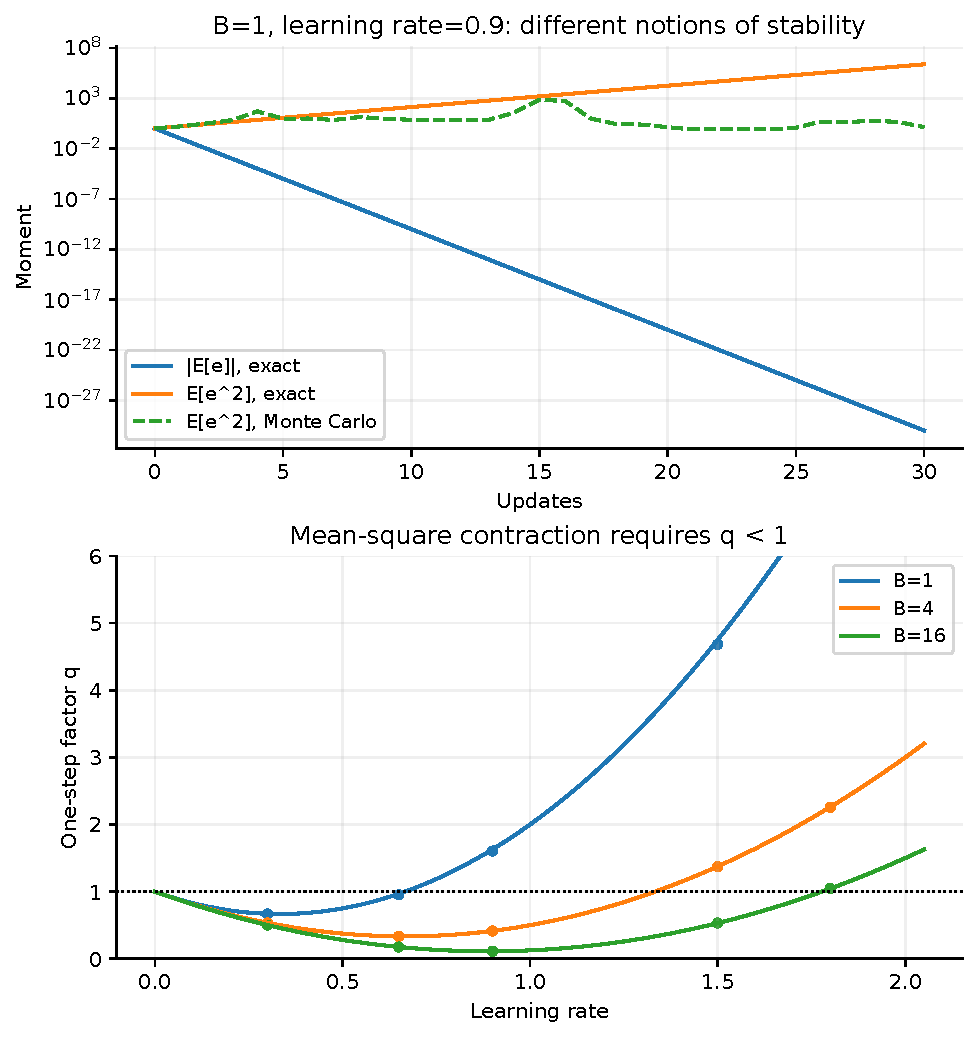
\includegraphics[width=0.85\textwidth]{figures/sgd_stability.pdf}
 \caption{随机回归中均值与均方稳定性的区别，以及单步二阶矩的理论预测与蒙特卡洛核验。解析结果来自本讲的精确矩递推；有限重复次数的蒙特卡洛估计带有抽样误差，特别是在乘性噪声较强时，不能把样本曲线与理论值的偏差直接解释为公式失效。}
 \label{l3:fig-stability}
\end{figure}

\subsection{实验步骤与提交物}

\begin{enumerate}
 \item \textbf{实现并核对梯度。} 设 $a_\star=2$、$s^2=1$、$\tau^2=1/4$。从 $a_0=3$ 出发，每一步重新生成 $x$ 与独立标签噪声。先用自动微分和显式公式 $g=Ae-b$ 在同一个批次上核对一次；损失使用批次平均，不能把求和损失混进学习率比较。
 \item \textbf{观察均值和均方的分离。} 对 $B=1$ 比较 $\eta=0.2$、$0.6$、$1.0$。并行运行多条独立轨迹，记录 $\widehat m_t$、$\widehat q_t$，叠加式\eqref{l3:mean-recurrence}与式\eqref{l3:finite-time-q}。用较短时间窗口观察不稳定组，避免溢出后仍把数值当成有效数据。
 \item \textbf{检查批量相关的边界。} 对 $B=1,4,16$，在各自理论边界 $2B/(B+2)$ 的两侧选择步长。记录均方误差是否收缩，并解释为什么只看平均参数不足以判断稳定。
 \item \textbf{检查线性缩放。} 比较固定学习率和固定 $\eta/B$ 两种设置，同时给出按步数与按已处理样本数排列的曲线。对稳定组报告有限时间理论值与实验值，不要求短轨迹已经到达稳态。
 \item \textbf{形成一页结论。} 每个结论都写明抽样方式、批量、步长、重复次数和预算口径。至少解释一个理论与实验偏差的可能来源，并设计一个能够区分解释的补充检查。
\end{enumerate}

\begin{center}
\small
\begin{tabularx}{\textwidth}{lXXX}
\toprule
应记录的量 & 回答的问题 & 理论对照 & 常见误读\\
\midrule
平均误差 $\widehat m_t$ & 有无平均方向偏差 & 式\eqref{l3:mean-recurrence} & 均值为零即稳定\\
二阶矩 $\widehat q_t$ & 平均风险是否受控 & 式\eqref{l3:finite-time-q} & 单轨迹平滑即可靠\\
样本数 $Bt$ & 数据使用效率 & 固定预算比较 & 每步更快即总训练更快\\
运行时间 & 实际资源效率 & 同设备重复测量 & 把启动开销当算法成本\\
\bottomrule
\end{tabularx}
\end{center}

\subsection{实验读图时的三个检查}

首先检查实现是否真的每步使用新样本。如果反复使用一个固定批次，观察的是另一随机问题。其次检查标签噪声的定义：若把 $\tau$ 当成方差传给要求标准差的生成器，预测的地板会改变。最后检查样本平均与总体期望的区别。稳定组可用更多独立重复缩小误差；不稳定乘性过程的少量极端轨迹可能支配二阶矩，不能通过删除极端值使曲线“符合直觉”。可以另报中位数，但必须保留它与二阶矩是不同统计量这一事实。

\section{习题}
\label{l3:exercises}

\begin{exercise}[抽样协方差]
\label{l3:ex-sampling}
固定 $N=100$ 个样本梯度，总体协方差采用分母 $N$，记为 $\Sigma_N$。分别求 $B=10$ 的有放回和不放回批次均值的协方差。解释为什么一个 epoch 内的随机重排不能在任意当前参数处直接使用条件无偏公式。
\end{exercise}

\begin{exercise}[精确均方递推]
\label{l3:ex-gaussian}
在高斯回归模型中，推导 $\E A_t^2$ 与 $\E b_t^2$。设 $s^2=2$、$B=2$、$\tau^2=1$，求均值稳定和均方稳定的步长区间，并计算 $\eta=0.2$ 时的稳态超额风险。
\end{exercise}

\begin{exercise}[稳态与有限时间]
\label{l3:ex-additive}
对加性噪声模型取 $\lambda=4$、$\sigma_g^2=8$、$B=16$。分别在 $\eta=0.05$ 与 $\eta=0.4$ 时计算稳态损失，并比较近似 $\eta\sigma_g^2/(4B)$ 的误差。说明为什么第二个步长虽稳定，近似却明显较差。
\end{exercise}

\begin{exercise}[非凸保证的适用范围]
\label{l3:ex-nonconvex}
重写式\eqref{l3:conditional-descent}的证明，指出在哪一步使用了条件无偏性、方差上界和光滑性。若希望 $\E\norm{\nabla F(w_R)}^2\leq\epsilon^2$，分别讨论确定性和固定批量随机情形由本讲上界给出的步数阶数。举例说明梯度为零不保证最小值。
\end{exercise}

\begin{exercise}[动量的参数约定]
\label{l3:ex-momentum}
设 $H$ 的特征值为 $1$ 和 $9$。对 Heavy Ball 取 $\beta=1/4$，求全部方向稳定的学习率区间，以及使所有方向同时位于复根区域内部的学习率区间。若改用 $m_t=\beta m_{t-1}+(1-\beta)g_t$，更新 $w_{t+1}=w_t-\alpha m_t$，求与原 Heavy Ball 步长 $\eta$ 等价的 $\alpha$。
\end{exercise}

\begin{exercise}[设计公平的 batch 实验]
\label{l3:ex-batch-design}
同学报告“$B=128$ 的训练损失在 1000 步时比 $B=32$ 低，因此大批量更高效”。给出该结论尚缺少的信息，并设计同时比较样本效率和运行时间效率的方案。在高斯模型中说明为什么即使保持 $\eta/B$，也不能预先保证两组稳态误差完全相同。
\end{exercise}

\section{习题解答要点}
\label{l3:solutions}

\subsection*{习题\ref{l3:ex-sampling}}
有放回协方差是 $\Sigma_N/10$。不放回协方差是
$90/(10\times99)\Sigma_N=\Sigma_N/11$。随机重排的下一批来自剩余样本，而当前参数已受先前样本影响；固定参数时的对称抽样计算，不等于关于训练历史条件化后的无偏性。

\subsection*{习题\ref{l3:ex-gaussian}}
将 $A_t^2$ 展开，$B$ 个同指标项使用 $\E x^4=3s^4$，$B(B-1)$ 个异指标项使用独立性，得到 $s^4(1+2/B)$。$b_t^2$ 的异指标项因标签噪声零均值而消失，得到 $s^2\tau^2/B$。均值稳定要求 $0<\eta<1$，均方稳定要求 $0<\eta<1/2$。取 $\eta=0.2$ 时，
\[
 q_\infty=\frac{0.2}{2[2-0.2\times2\times2]}=\frac1{12}.
\]
超额风险是 $s^2q_\infty/2=1/12$，另外还存在不可约损失 $\tau^2/2$。

\subsection*{习题\ref{l3:ex-additive}}
稳定范围为 $0<\eta<1/2$。精确稳态损失分别为
$0.4/[32(1.8)]=1/144\approx0.006944$ 和
$3.2/[32(0.4)]=1/4$。小步长近似分别为 $0.00625$ 和 $0.05$。第二组的 $\eta\lambda=1.6$ 并不小，分母 $2-\eta\lambda$ 不能用 $2$ 替代。

\subsection*{习题\ref{l3:ex-nonconvex}}
光滑性用于二阶上界；条件无偏性同时用于交叉项和二阶矩分解；方差上界控制剩余噪声项。确定性情形取 $\eta=1/L$，达到梯度平方精度 $\epsilon^2$ 的上界为 $O(\epsilon^{-2})$ 步。固定 $B$ 的一般随机情形，平衡两项后需要 $O(\epsilon^{-4})$ 步。这些阶数将 $L,\Delta,\sigma,B$ 看作固定量。$F(w)=1-\cos w$ 在 $w=\pi$ 处梯度为零但为局部最大值，是直接反例。

\subsection*{习题\ref{l3:ex-momentum}}
稳定区间为 $0<\eta<2(1+1/4)/9=5/18$。复根要求对 $\lambda=1$ 有 $\eta>1/4$，对 $\lambda=9$ 有 $\eta<(3/2)^2/9=1/4$，严格区间为空；在 $\eta=1/4$ 时两个端点恰好成为重根，这也是本例经典最优二次参数。若两种动量均从零开始，$m_t=(1-\beta)v_t$，所以 $\alpha=\eta/(1-\beta)=4\eta/3$。

\subsection*{习题\ref{l3:ex-batch-design}}
原比较使用了四倍样本，且尚未说明设备、吞吐、学习率、初始化、目标精度和重复次数。应固定模型、数据及随机种子集合，分别画损失对已处理样本数和损失对运行时间的曲线，并比较到达同一阈值的成本。高斯模型的精确地板除 $\eta/B$ 外，还含 $2-\eta s^2(1+2/B)$；保持比值不保持分母。可以在足够小的步长下提出近似相同的预测，再用实验检查近似误差。

\begin{coursebox}{离开本讲时应保留的判断顺序}
先定义目标与抽样，再检查均值和二阶矩，随后说明收敛指标与计算预算。对动量，先写完整状态递推和学习率约定，再判断稳定区域。进入深度网络后，可以使用这些小模型形成可检验的预测，但需要重新核对其假设，不能把模型中的充分条件或近似规律直接称为所有网络的训练定律。
\end{coursebox}

\chapter{预条件、自适应优化与矩阵更新}
\label{l4:chapter}

\begin{coursebox}{学习目标与课时安排}
本讲安排为一个半理论学时和一个半实验学时。核心问题是：参数空间中什么叫“一小步”，不同的定义如何产生不同更新方向？理论核心依次是二次度量、对偶范数、谱范数球与 polar 方向；AdaGrad、AdamW 和 Muon 用于说明这些理想模型如何进入带有历史状态的实际算法。

自然梯度、K-FAC、Shampoo 以及更新相关性的稳态推导列为选读。实验必须区分精确 SVD 参考、有限步 Newton--Schulz 近似、辅助参数更新和学习率尺度约定。学完本讲，应能从一个更新公式识别其几何、历史状态和数值近似，并能设计公平的优化器比较。
\end{coursebox}

\section{同一个梯度，什么叫同样大小的一步}
\label{l4:metric}

设目标为 $F(w)$，当前梯度为 $g=\nabla F(w)$。一阶近似告诉我们，小位移 $d$ 引起的损失变化约为 $\inner{g}{d}$，但只最小化这个线性函数会沿某个方向无限前进。下降方法必须限制位移，或者惩罚过大的位移。限制的方式决定了“最陡”的含义。

先考虑二次惩罚模型
\begin{equation}
 d_\star=\argmin_{d\in\R^p}
 \left\{\inner{g}{d}+\frac1{2\eta}d^\top M d\right\},
 \qquad M\succ0.
 \label{l4:quadratic-model}
\end{equation}
对 $d$ 求导可得唯一解
\begin{equation}
 \boxed{d_\star=-\eta M^{-1}g=-\eta Pg},\qquad P=M^{-1}.
 \label{l4:preconditioned-step}
\end{equation}
矩阵 $M$ 定义了位移的度量，$P$ 是预条件矩阵。$M=I$ 给出普通梯度下降；$M$ 在某一方向大，表示该方向的位移昂贵，因此相应更新更小。这里 $M$ 必须正定，否则二次模型不一定有有限最小值。

若使用变量替换 $z=M^{1/2}w$，在 $z$ 坐标中进行普通梯度下降，再换回 $w$，恰好得到式\eqref{l4:preconditioned-step}。因此预条件也可理解为选择适合问题的坐标。它不会改变目标函数的最优解集合，却会改变达到最优解的路径与速度；在欠定或非凸问题中，路径变化还可能影响最终选中的解。

\subsection{曲率与稳定性如何变化}

对固定二次目标 $F(w)=\tfrac12(w-w_\star)^\top H(w-w_\star)$，设 $H\succ0$ 且 $P\succ0$ 固定。误差更新为
\[
 e_{t+1}=(I-\eta PH)e_t.
\]
虽然 $PH$ 不必对称，它与对称正定矩阵 $P^{1/2}HP^{1/2}$ 相似。因此迭代的稳定条件为
\begin{equation}
 0<\eta<\frac{2}{\lambda_{\max}(P^{1/2}HP^{1/2})}.
 \label{l4:preconditioned-stability}
\end{equation}
有效条件数也由这个矩阵决定。若 $P=H^{-1}$，则全部特征值等于一，$\eta=1$ 一步到达二次目标的最优点。这是 Newton 方法最清楚的理想情形。对非凸目标，Hessian 可能不定；对自适应方法，$P$ 随历史变化，不能直接用一个固定矩阵的结论覆盖整个训练过程\citep{Nocedal2006}。

\begin{example}[改变度量解决各向异性]
令
\[
 F(w)=\frac12(100w_1^2+w_2^2),\qquad w_0=(1,1)^\top.
\]
普通 GD 的稳定步长必须小于 $0.02$。取 $\eta=0.01$，得到
$w_1=(0,0.99)^\top$：陡方向已经到零，平缓方向只前进了百分之一。若使用 $M=\diag(100,1)$ 和 $\eta=1$，则
$d=-M^{-1}\nabla F(w_0)=(-1,-1)^\top$，一步达到零。

这个例子说明预条件的目标是改善相关的曲率比例，而不是单纯让所有坐标更新幅度相同。后面 Adam 的梯度二阶矩与 Hessian 不是同一个量，因此不能把 Adam 的对角分母直接称为 Hessian 的对角近似。
\end{example}

\section{对偶范数与最陡下降方向}
\label{l4:dual-norm}

二次模型是一条路线，另一条路线是给位移一个硬约束。给定一个范数 $\psi$，考虑
\begin{equation}
 \min_{\psi(d)\leq\rho}\inner{g}{d},\qquad\rho>0.
 \label{l4:norm-ball}
\end{equation}
这里使用闭球，使有限维连续优化问题取得最小值。若改成严格不等式 $\psi(d)<\rho$，非零线性目标通常只有下确界而没有最小点。

\begin{definition}[对偶范数]
范数 $\psi$ 的对偶范数为
\begin{equation}
 \psi_*(g)=\max_{\psi(u)\leq1}\inner{g}{u}.
 \label{l4:dual-norm-definition}
\end{equation}
它衡量单位位移预算下，线性目标能够变化多大。
\end{definition}

\begin{proposition}[范数球内的线性最小化]
式\eqref{l4:norm-ball}的最优值是 $-\rho\psi_*(g)$。若
$u_\star\in\argmax_{\psi(u)\leq1}\inner{g}{u}$，则
$d_\star=-\rho u_\star$ 是一个最优解。解不必唯一。
\end{proposition}
\begin{proof}
范数的对称性和变量代换 $d=-\rho u$ 给出
\[
 \min_{\psi(d)\leq\rho}\inner{g}{d}
 =-\rho\max_{\psi(u)\leq1}\inner{g}{u}
 =-\rho\psi_*(g).
\]
有限维闭单位球紧致，连续目标取得最大值，故上述方向存在。
\end{proof}

对 $g\ne0$，几个典型选择为
\begin{center}
\small
\begin{tabularx}{\textwidth}{lXXX}
\toprule
位移约束 & 对偶范数 & 一个最优方向 $d_\star$ & 解释\\
\midrule
$\norm{d}_2\leq\rho$ & $\norm{g}_2$ & $-\rho g/\norm{g}_2$ & 固定总欧氏长度\\
$\norm{d}_\infty\leq\rho$ & $\norm{g}_1$ & $-\rho\operatorname{sign}(g)$ & 各坐标各有预算\\
$\norm{d}_1\leq\rho$ & $\norm{g}_\infty$ & $-\rho\operatorname{sign}(g_j)e_j$ & 预算集中在最大梯度坐标\\
\bottomrule
\end{tabularx}
\end{center}
第三行取 $j\in\argmax_i|g_i|$；并列最大时可以有多个解。第二行在零梯度坐标上也不唯一，约定 $\operatorname{sign}(0)=0$ 即可得到一个解。若 $g=0$，整个约束球都是最优解，不能使用包含 $1/\norm{g}$ 的公式。

\begin{example}[同一个梯度对应三种预算]
令 $g=(3,-1)^\top$，$\rho=0.1$。欧氏球给出
\[
 d_2=\frac{0.1}{\sqrt{10}}(-3,1)^\top,
 \qquad \inner{g}{d_2}=-0.1\sqrt{10}.
\]
无穷范数球给出 $d_\infty=(-0.1,0.1)^\top$，线性变化为 $-0.4$；一范数球给出 $d_1=(-0.1,0)^\top$，线性变化为 $-0.3$。

这不能直接证明其中某个算法更好，因为三种可行集不同。例如 $\norm{d_\infty}_2=\sqrt2\rho$，已经超过欧氏球的半径。比较更新时，应说明保持的是哪一种尺度，不能只比较公式中的同一个 $\rho$ 数值。
\end{example}

\begin{figure}[htbp]
 \centering
 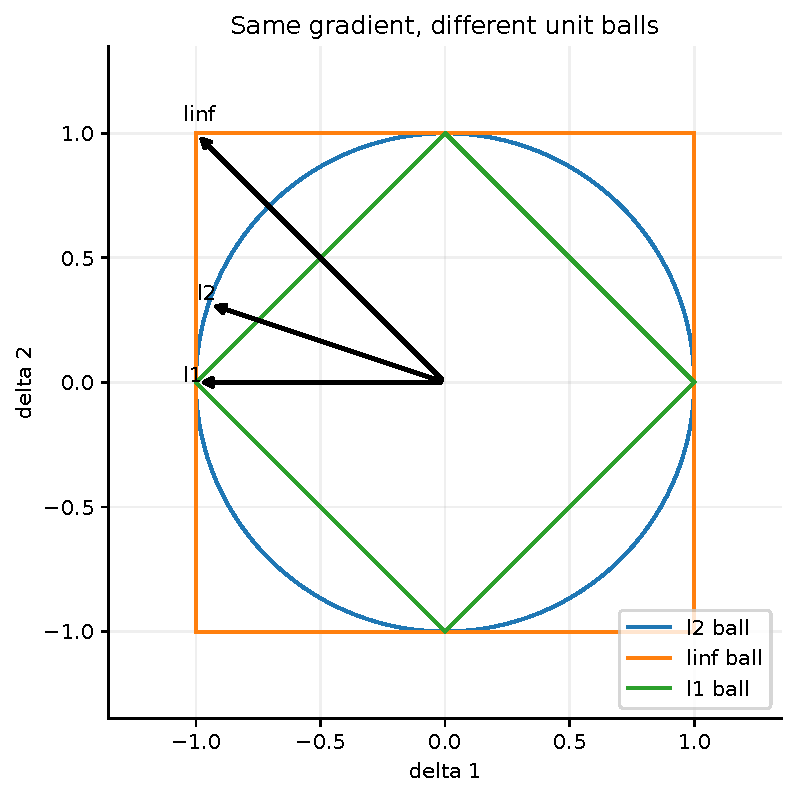
\includegraphics[width=0.7\textwidth]{figures/norm_geometry.pdf}
 \caption{同一梯度在不同闭范数球上的精确线性最小化方向。相同的半径数值对应不同的可行位移集合，因此方向与一阶下降量也不同。这幅图比较的是局部几何模型，完整算法还需指定梯度估计、历史状态和步长。}
 \label{l4:fig-norm-geometry}
\end{figure}

\subsection{方向归一化与普通 GD 的区别}

欧氏球给出的是\emph{归一化梯度方向}，普通 GD 则来自二次惩罚。二者的步长一个控制长度，一个乘在原始梯度上。为了看清一般关系，考虑
\begin{equation}
 \min_d\left\{\inner{g}{d}+\frac{\psi(d)^2}{2\eta}\right\}.
 \label{l4:squared-norm-model}
\end{equation}
对固定半径 $r=\psi(d)$，线性项的最优值为 $-r\psi_*(g)$；再对 $r\geq0$ 最小化
$-r\psi_*(g)+r^2/(2\eta)$，得到
\[
 r_\star=\eta\psi_*(g),\qquad
 d_\star=-\eta\psi_*(g)u_\star.
\]
因此同一个范数，配合固定半径或平方范数惩罚，也会给出不同的更新长度。这是后面统一理解算法时必须保留的细节。

\begin{coursebox}{“范数统一优化器”应当怎样理解}
不同范数定义了几类理想最陡下降方向。实际算法还要指定梯度估计、动量、历史统计量、步长、权重衰减和数值实现。对偶范数可以解释一个方向为什么出现，但仅凭方向相似，不能把两个完整算法的稳定性和收敛定理互相移植。
\end{coursebox}

\section{从累积二阶矩到 Adam}
\label{l4:adaptive}

\subsection{AdaGrad 与 RMSProp 的历史统计量}

为避免时间下标歧义，本节在参数 $w_{t-1}$ 处计算梯度 $g_t$，随后产生 $w_t$，初始状态下标为零。逐元素运算用 $\odot$ 或分量公式表示。
AdaGrad 维护累积平方梯度\citep{Duchi2011}
\begin{equation}
 s_t=s_{t-1}+g_t\odot g_t,
 \qquad
 w_t=w_{t-1}-\eta\frac{g_t}{\sqrt{s_t}+\epsilon},
 \label{l4:adagrad}
\end{equation}
其中分式与平方根都按分量计算，$\epsilon>0$ 用于避免数值除零。长期出现较大梯度的坐标获得较小的有效步长；很少出现梯度的坐标则不会仅因其他坐标更新频繁而被同等压低。其累积结构也会使分母持续增大，是否符合任务需要取决于训练阶段。

RMSProp 用指数平均代替无限累积：
\begin{equation}
 v_t=\beta_2v_{t-1}+(1-\beta_2)g_t\odot g_t,
 \qquad
 w_t=w_{t-1}-\eta\frac{g_t}{\sqrt{v_t}+\epsilon}.
 \label{l4:rmsprop}
\end{equation}
指数平均可以追踪变化的梯度尺度，但有限记忆也改变了理论条件。AdaGrad 的某个收敛证明不能仅将累积和替换成指数平均后原样保留。这里的 $v_t$ 是\emph{梯度平方的统计量}，不是 Hessian 的特征值或方差本身；非零均值时二阶矩与方差也不同。

\subsection{Adam 的完整状态方程}

Adam 同时使用一阶矩和二阶矩状态\citep{Kingma2015}：
\begin{align}
 m_t&=\beta_1m_{t-1}+(1-\beta_1)g_t,\notag\\
 v_t&=\beta_2v_{t-1}+(1-\beta_2)g_t\odot g_t,\notag\\
 \widehat m_t&=\frac{m_t}{1-\beta_1^t},\qquad
 \widehat v_t=\frac{v_t}{1-\beta_2^t},\notag\\
 u_t&=\frac{\widehat m_t}{\sqrt{\widehat v_t}+\epsilon},\qquad
 w_t=w_{t-1}-\eta_tu_t.
 \label{l4:adam}
\end{align}
这里 $m_0=v_0=0$，$0\leq\beta_1,\beta_2<1$。偏差修正补偿零初始状态对恒定均值矩估计的初期影响；它不保证当梯度分布变化时，矩估计就是当前真实矩。

若把 $D_t=\diag(\sqrt{\widehat v_t}+\epsilon)$，则 Adam 更新是
$-\eta_tD_t^{-1}\widehat m_t$。这可以看作对\emph{带记忆的方向}施加对角预条件，不能一般写成对当前真实梯度使用某个 Hessian 逆矩阵。

\subsection{哪些情况下才出现 SignGD}

设 $\beta_1=\beta_2=0$ 且忽略 $\epsilon$，对于非零梯度分量，式\eqref{l4:adam}严格给出
\[
 u_t=\frac{g_t}{|g_t|}=\operatorname{sign}(g_t).
\]
零分量约定更新为零。另一个可检验的特例是从第一步开始梯度始终等于同一个非零常向量，此时偏差修正后 $\widehat m_t=g$、$\widehat v_t=g^2$，也得到 sign 方向。实际训练中可以用这个极限解释逐坐标归一化的倾向，但“目标是二次函数”并不足以使历史梯度保持不变。

\begin{example}[Adam 的方向可以与当前 sign 不同]
考察一个坐标，设 $m_0=v_0=0$、$\beta_1=\beta_2=0.9$，忽略 $\epsilon$。两次梯度分别为 $g_1=1$、$g_2=-0.1$。第二步有
\[
 m_2=0.08,\qquad v_2=0.091,
 \qquad\widehat m_2=\frac{0.08}{0.19},
 \qquad\widehat v_2=\frac{0.091}{0.19}.
\]
因此 $u_2\approx0.6084>0$，Adam 使参数减小；当前梯度为负，SignGD 则使参数增大。两步就足以看出历史状态的重要性。这也不意味着 Adam 在整个过程中一定更差：动量可能暂时抵抗一个新方向；是否有益需要考察后续动力学。
\end{example}

在对角正定二次函数上，固定步长 SignGD 的每个坐标最终进入一个宽度与步长成比例的区间，并通常形成二周期。这是有界性分析，不是收敛到最优点的证明，也不是完整 Adam 的稳定性定理。Adam 的收敛需要额外条件；已有工作给出了简单凸随机优化环境中不能收敛到最优解的反例及相应修正\citep{Reddi2018}。课堂上应以这些反例提醒学生核对假设，不能反过来解释为任何使用 Adam 的训练都会失败。

\subsection{坐标与学习率的单位}

把损失整体乘以正数 $c$，普通 GD 的梯度和位移都会乘以 $c$；在 $\epsilon$ 可忽略且状态同样缩放的理想条件下，Adam 的 $m$ 乘以 $c$、$v$ 乘以 $c^2$，比值近似不变。因此 Adam 与 SGD 的学习率数值不能直接比较。学习率 $10^{-3}$ 比 $10^{-2}$ 小，并不意味着参数实际走得更短。

逐坐标方法也依赖坐标系。例如取 $g=(1,2)^\top$ 和
\[
 Q=\frac1{\sqrt2}
 \begin{pmatrix}1&-1\\1&1\end{pmatrix}.
\]
则 $Q\operatorname{sign}(g)=(0,\sqrt2)^\top$，但
$\operatorname{sign}(Qg)=(-1,1)^\top$。先旋转梯度再取 sign，与先取 sign 再旋转不相同。这不是一个实现缺陷，而是选择坐标范数的几何后果。

\section{AdamW 与自适应 L2 正则}
\label{l4:adamw}

对普通梯度下降，把目标改成 $F(w)+\lambda\norm{w}^2/2$ 会得到
\[
 w_t=(1-\eta_t\lambda)w_{t-1}-\eta_t\nabla F(w_{t-1}).
\]
因此在这一个特定算法中，L2 正则与乘性权重衰减等价。预条件出现后，情况改变。若暂时固定 $P$，耦合 L2 更新是
\begin{equation}
 w_t=w_{t-1}-\eta_tP\bigl(g_t+\lambda w_{t-1}\bigr),
 \label{l4:coupled-l2}
\end{equation}
而解耦衰减是
\begin{equation}
 w_t=(1-\eta_t\lambda)w_{t-1}-\eta_tPg_t.
 \label{l4:decoupled-decay}
\end{equation}
除非预条件与正则形式满足特别关系，两式不同。在 Adam 中，若将 $\lambda w$ 加进梯度，它还会进入 $m_t,v_t$ 的历史统计量，差异更大。

AdamW 用来自原目标梯度的 $u_t$，并另外施加衰减\citep{Loshchilov2019}：
\begin{equation}
 \boxed{w_t=(1-\eta_t\lambda)w_{t-1}-\eta_tu_t}.
 \label{l4:adamw-rule}
\end{equation}
这里约定 $\lambda$ 是与学习率相乘的衰减系数。有些实现直接传入每步收缩量，或对不同参数组设置不同的衰减；比较配置前必须核对定义。

\begin{example}[两种正则化的收缩不同]
取当前 $w=(1,1)^\top$、数据梯度 $g=0$、固定
$P=\diag(0.01,1)$、$\eta=0.1$、$\lambda=1$。
耦合 L2 更新得到 $(0.999,0.9)^\top$，解耦衰减得到 $(0.9,0.9)^\top$。第一种规则在预条件较小的方向上也更少收缩，第二种规则使用相同的相对收缩比例。

这个例子只比较两个明确更新公式，不说明哪一种必然泛化更好。对真实网络，还需说明 bias、归一化参数和输出层是否衰减，以及学习率随时间变化后累计收缩量如何变化。
\end{example}

\section{矩阵参数：谱范数球与 polar 方向}
\label{l4:spectral-ball}

神经网络的一层常由矩阵 $W\in\R^{m\times n}$ 表示。将它展平成向量当然可以使用前面的算法，但矩阵本身还具有输入、输出和奇异方向的结构。记矩阵梯度为 $G$，Frobenius 内积为
$\inner{G}{D}_F=\tr(G^\top D)$。

矩阵谱范数与核范数分别为
\[
 \norm{D}_{\rm op}=\max_{\norm{x}_2\leq1}\norm{Dx}_2,
 \qquad
 \norm{G}_*=\sum_{i=1}^{\rank(G)}\sigma_i(G).
\]
谱范数控制一个线性映射对任何输入方向的最大放大，核范数是其对偶范数。这一对偶关系使矩阵更新具有一个简洁的精确解。

\begin{theorem}[谱范数球内的最优线性方向]
令 $G=U_r\Sigma_rV_r^\top$ 为秩 $r>0$ 的紧致 SVD，$\Sigma_r$ 的对角元严格为正。则
\begin{equation}
 \min_{\norm{D}_{\rm op}\leq\rho}\inner{G}{D}_F
 =-\rho\norm{G}_*,
 \qquad
 D_\star=-\rho U_rV_r^\top
 \label{l4:polar-optimum}
\end{equation}
给出一个最优解。称 $Q(G)=U_rV_r^\top$ 为本讲采用的 canonical polar 方向，并约定 $Q(0)=0$。
\end{theorem}
\begin{proof}
将 $G$ 写成 $\sum_{i=1}^r\sigma_i u_i v_i^\top$，则任意可行 $D$ 满足
\[
 \inner{G}{D}_F=\sum_{i=1}^r\sigma_i u_i^\top Dv_i
 \geq-\sum_{i=1}^r\sigma_i\norm{D}_{\rm op}
 \geq-\rho\sum_{i=1}^r\sigma_i.
\]
对 $D_\star=-\rho U_rV_r^\top$，每个 $u_i^\top D_\star v_i=-\rho$，且其谱范数为 $\rho$，所以达到下界。
\end{proof}

谱范数单位球包含所有收缩映射，\emph{不是正交矩阵集合}。上面的一个最优解恰好把非零梯度奇异方向上的奇异值变为一。若矩阵满秩且 $m\geq n$，有 $Q^\top Q=I_n$；若满秩且 $m\leq n$，有 $QQ^\top=I_m$。秩亏时，这两个乘积对应子空间投影，不能都写成单位阵。零梯度奇异方向没有一阶偏好，因此最优解可能不唯一。

\begin{example}[矩阵 sign 与逐元素 sign 不同]
设
\[
 G=\begin{pmatrix}3&0&0\\0&1&0\end{pmatrix}.
\]
其 polar 方向为
\[
 Q(G)=\begin{pmatrix}1&0&0\\0&1&0\end{pmatrix}.
\]
谱球半径为 $\rho$ 时，线性变化是 $-4\rho$。Frobenius 球半径为 $\rho$ 时，方向为 $-\rho G/\sqrt{10}$，线性变化为 $-\sqrt{10}\rho$。差别来自预算的含义，不能脱离约束直接解读为某个更新总是更好。

再取一个列向量 $g=(3,4)^\top$，把它视为 $2\times1$ 矩阵，则 $Q(g)=g/5$，而逐元素 $\operatorname{sign}(g)=(1,1)^\top$。所以“矩阵 sign 在向量上就是逐元素 sign”一般不成立。两者分别归一化奇异值和坐标幅度。
\end{example}

polar 方向不需要 Hessian 信息，因此不能仅因它把奇异值整平，就称它为 Newton 方向。它也可能放大相对较弱的梯度奇异方向；这些方向究竟是有用信号还是噪声，需要数据和训练实验判断，低奇异值并不自动等于噪声。

\section{RMS 诱导范数与数据方向}
\label{l4:rms-induced}

对 $x\in\R^n$，定义
$\operatorname{RMS}(x)=\norm{x}_2/\sqrt n$；对 $W\in\R^{m\times n}$，逐元素 RMS 定义为
$\operatorname{RMS}(W)=\norm{W}_F/\sqrt{mn}$。两者都在测量每个元素的典型量级，但矩阵的\emph{逐元素 RMS}与它作为映射的\emph{RMS 诱导范数}是两个量。

\begin{proposition}[RMS 到 RMS 的诱导范数]
对 $W:\R^n\to\R^m$，
\begin{equation}
 \norm{W}_{\mathrm{RMS}\to\mathrm{RMS}}
 :=\sup_{x\ne0}\frac{\operatorname{RMS}(Wx)}{\operatorname{RMS}(x)}
 =\sqrt{\frac nm}\norm{W}_{\rm op}.
 \label{l4:rms-operator}
\end{equation}
\end{proposition}
\begin{proof}
比值等于 $\sqrt{n/m}\norm{Wx}_2/\norm{x}_2$，对 $x$ 取上确界即可。
\end{proof}

如果希望对所有输入都保证
\[
 \operatorname{RMS}(\Delta W x)\leq
 \rho\operatorname{RMS}(x),
\]
可以施加 $\norm{\Delta W}_{\rm op}\leq\rho\sqrt{m/n}$，其最陡方向为
\begin{equation}
 \Delta W=-\rho\sqrt{\frac mn}Q(G).
 \label{l4:rms-steepest}
\end{equation}
这是一个最坏输入方向的扰动上界，不保证实际输入的特征一定改变相同量级，也不直接保证整个网络的损失下降。若当前输入落在 $\Delta W$ 的零空间，实际扰动就是零。第五讲讨论跨宽度的非退化特征变化时，还需要输入与更新方向的对齐信息。

\subsection{从最坏方向到实际数据，选读}

如果输入二阶矩为 $C=\E[xx^\top]$，则有精确恒等式
\begin{equation}
 \E\norm{Dx}_2^2=\tr(DCD^\top).
 \label{l4:data-perturbation}
\end{equation}
这里不要求 $x$ 零均值，$C$ 是二阶矩；只有零均值时它才等于协方差。于是可以考虑一个按数据扰动惩罚的局部模型
\[
 \min_D\left\{\inner{G}{D}_F+
 \frac{1}{2\eta}\tr(DCD^\top)\right\}.
\]
当 $C\succ0$ 时，它的唯一解为
\begin{equation}
 D_\star=-\eta GC^{-1}.
 \label{l4:data-preconditioning}
\end{equation}
这把数据几何和预条件直接连接起来：高能量输入方向上的同样权重变化会产生更大的平均输出扰动，因此受到更强惩罚。若 $C$ 奇异，可在其支撑子空间分析，或显式加入阻尼 $\gamma I$；不应直接写一个不存在的逆。

\begin{example}[按照数据能量调整更新]
设一层只有一个输出，输入二阶矩为 $C=\diag(100,1)$，当前梯度行为 $G=(1,1)$。欧氏二次惩罚给出 $D=-\eta(1,1)$；数据扰动惩罚给出 $D=-\eta(0.01,1)$。这不是根据坐标名称任意修改步长，而是因为第一个输入方向的二阶能量大一百倍。

真实网络中还存在输出损失的度量和跨层耦合，因此这个例子不是完整网络的最优预条件器。它给出一个可迁移的设计问题：应该控制参数变化，还是控制参数变化对当前数据产生的函数变化？
\end{example}

\section{实际 Muon：动量、polar 与数值近似}
\label{l4:muon}

Muon 将矩阵动量转成近似正交化的更新方向。其发展与规模化应用可参见\citet{Jordan2024}和\citet{Liu2025}。不同实现会使用不同的动量约定、矩阵形状缩放和近似多项式；因此本讲先给出一个可完全复现的版本。

对矩阵参数 $W\in\R^{m\times n}$，定义
\begin{align}
 G_t&=\nabla_W F(W_{t-1}),\notag\\
 M_t&=\beta M_{t-1}+(1-\beta)G_t,\notag\\
 Q_t&=Q(M_t)\quad\hbox{或其明确指定的数值近似},\notag\\
 W_t&=(1-\eta_t\lambda)W_{t-1}-\eta_t a(m,n)Q_t.
 \label{l4:muon-reference}
\end{align}
随机训练时以批次梯度替换 $G_t$。这个版本使用 EMA 动量，不额外使用 Nesterov 外推。精确 polar 对正的整体比例不敏感，所以在零初始状态下，省略 EMA 中的 $1-\beta$ 不改变精确方向；但初始化、阻尼和数值归一化仍须一致。把同一观察移植到 Adam 的两种状态上则需要另外检查。

式\eqref{l4:polar-optimum}解释的是以 $M_t$ 为线性目标的最优方向。因为 $M_t$ 不一定与当前 $G_t$ 一致，不能据此保证每一步都最大化\emph{当前损失}的一阶下降。实际 Muon 的动力学还包含记忆、步长和近似误差。

\subsection{用 SVD 构造参考答案}

小矩阵可以直接做 SVD，并把非零奇异值替换成一。这一版本适合验证方向和误差，不一定适合大规模训练。秩亏时，应将零奇异值保留为零，得到 canonical polar。浮点实现需要明确判断有效零奇异值的阈值；库返回的完整奇异向量基不应使理论零方向凭空获得更新。

\subsection{三次 Newton--Schulz 迭代}

若 $M\ne0$，令 $X_0=M/\norm{M}_F$，并迭代
\begin{equation}
 X_{k+1}=\frac32X_k-\frac12X_kX_k^\top X_k.
 \label{l4:ns-cubic}
\end{equation}
矩阵乘法的结合次序可按形状选取较小的 Gram 矩阵：$m\leq n$ 时计算 $(X_kX_k^\top)X_k$，$m>n$ 时计算 $X_k(X_k^\top X_k)$。两者在精确算术中相同。若 $M=0$，直接返回零。

\begin{proposition}[三次迭代的奇异值行为]
在精确算术中，式\eqref{l4:ns-cubic}保留初始奇异向量。每个奇异值按
\begin{equation}
 s_{k+1}=p(s_k),\qquad p(s)=\frac32s-\frac12s^3
 \label{l4:ns-scalar}
\end{equation}
变化。若 $0<s_0\leq1$，则 $s_k\to1$；若 $s_0=0$，则一直为零。因此 $X_k$ 趋于 canonical polar 方向。
\end{proposition}
\begin{proof}
将 SVD 代入矩阵多项式即可得到奇异值递推。对于 $0<s<1$，
$p(s)-s=\tfrac12s(1-s^2)>0$，并且
\[
 1-p(s)=\frac12(1-s)^2(s+2)>0.
\]
所以奇异值单调上升且不超过一，极限必须满足 $p(s)=s$；正初值的极限只能为一。Frobenius 归一化保证所有初始奇异值不超过一。
\end{proof}

有限次迭代不等于极限。特别小的奇异值初期大约每次乘以 $1.5$，五步未必足以将它推近一。因此实验中的 NS5 既可以比 SVD 更便宜，也可能明显改变弱奇异方向。原始及竞速实现常使用为固定计算预算设计的其他多项式；其有限步变换不应直接套用本节三次迭代的收敛证明。

\begin{example}[五步与极限的差别]
设某个矩阵归一化后，其中两个奇异值分别为 $0.9$ 和 $0.01$。第一个值已接近一，且误差因式 $1-p(s)=\tfrac12(1-s)^2(s+2)$ 快速减小。第二个值在早期近似按 $0.01\times1.5^k$ 增长，五步后仍只约为 $0.076$ 的量级。

因此“运行了 Newton--Schulz”不能替代对近似质量的说明。应记录 $\norm{X_K-Q(M)}_F$ 或奇异值分布，并区分满秩和秩亏情况。对秩亏矩阵，$X_K^\top X_K-I$ 本来就不可能趋零，不宜把这个量无条件作为正确性判据。
\end{example}

\begin{figure}[htbp]
 \centering
 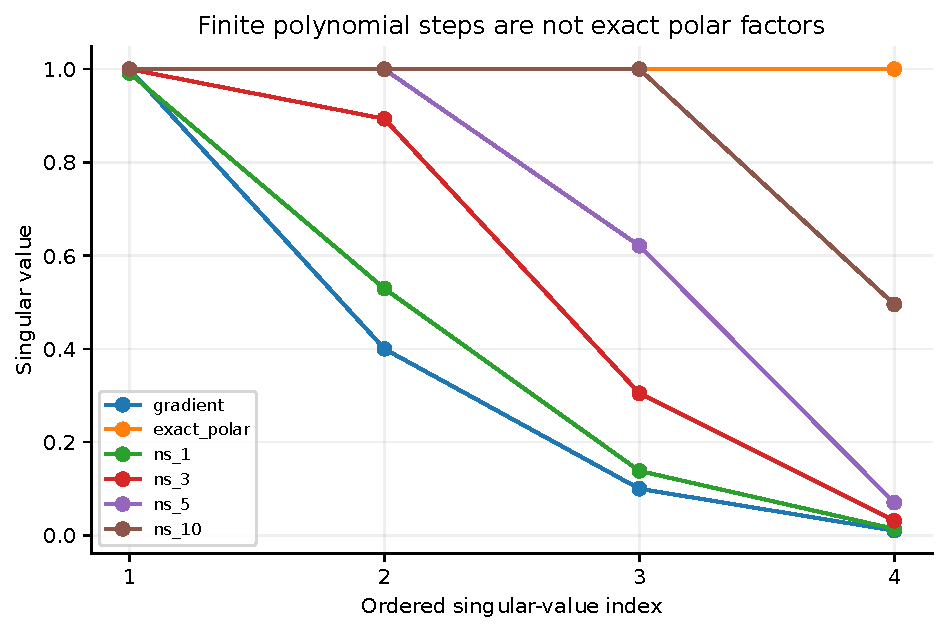
\includegraphics[width=0.85\textwidth]{figures/polar_approximation.pdf}
 \caption{有限步三次 Newton--Schulz 迭代与 SVD 构造的 canonical polar 参考之间的区别。精确 polar 将非零奇异值变为一，并使零奇异方向保持为零；有限步近似在小奇异值方向上可能仍明显偏离参考。因此 NS 步数、初始归一化和数值精度都是所比较算法的一部分。}
 \label{l4:fig-polar-approximation}
\end{figure}

\section{更新 RMS：一种工程尺度，而非迁移定理}
\label{l4:rms-matching}

\subsection{三种缩放约定}

对秩为 $r$ 的 canonical polar 矩阵 $Q\in\R^{m\times n}$，有
\begin{equation}
 \norm{Q}_F^2=r,
 \qquad\operatorname{RMS}(Q)=\sqrt{\frac{r}{mn}}.
 \label{l4:polar-rms}
\end{equation}
若满秩，即 $r=\min(m,n)$，逐元素 RMS 为 $1/\sqrt{\max(m,n)}$。因此以下三个缩放各有不同含义：
\begin{center}
\small
\begin{tabularx}{\textwidth}{lXX}
\toprule
名称 & 式\eqref{l4:muon-reference}中的 $a(m,n)$ & 控制或对齐的尺度\\
\midrule
裸 polar & $1$ & 矩阵更新的谱范数\\
RMS 诱导范数约定 & $\sqrt{m/n}$ & 最坏输入方向的相对 RMS 扰动\\
逐元素 RMS 匹配 & $c\sqrt{\max(m,n)}$ & 满秩精确 polar 的逐元素 RMS 为 $c$\\
\bottomrule
\end{tabularx}
\end{center}
本讲 GPU 实验采用第三种约定，取 $c=0.2$。满秩且使用精确 polar 时，未乘学习率的更新 RMS 恰为 $0.2$；秩亏或有限步 NS 时不必精确等于该值。比较宽度、矩阵形状和学习率时，应同时保留 $a(m,n)$，不能仅抄一个名义学习率。

\subsection{为什么有时观察到 Adam 更新 RMS 接近 $0.2$}

先分析一个用于建立直觉的理想噪声模型。单坐标梯度在时间上独立同分布，均值为零、方差为 $\sigma_g^2>0$；忽略初始瞬态和 $\epsilon$。在稳态，Adam 的两个 EMA 满足
\begin{equation}
 \E m_t^2=\frac{1-\beta_1}{1+\beta_1}\sigma_g^2,
 \qquad \E v_t=\sigma_g^2.
 \label{l4:adam-moment-rms}
\end{equation}
分母和分子由同一历史梯度产生，通常相关，故下面是\emph{近似}而非恒等式：
\begin{equation}
 \E\left[\frac{m_t^2}{v_t}\right]
 \approx\frac{\E m_t^2}{\E v_t}
 =\frac{1-\beta_1}{1+\beta_1}.
 \label{l4:mean-field-rms}
\end{equation}
取 $\beta_1=0.9$，由此预测更新 RMS 约为
$\sqrt{0.1/1.9}\approx0.2294$。它解释了一个可能的量级，并不证明所有数据、模型和训练阶段都具有这个数值。

若第 $j$ 个坐标有非零均值 $\mu_j$ 和噪声方差 $\sigma_j^2$，同样近似给出
\[
 \E u_j^2\approx
 \frac{\mu_j^2+\frac{1-\beta_1}{1+\beta_1}\sigma_j^2}
 {\mu_j^2+\sigma_j^2}.
\]
整体逐元素 RMS 平方应再对这些\emph{比值}作坐标平均，一般不能直接改成两个总和的比值。恒定非零梯度的极限给出更新 RMS 接近一；时间相关的噪声也会改变 $m_t$ 的方差。$\beta_2$ 在式\eqref{l4:mean-field-rms}中消失，是近似结构造成的，不能推断真实分布完全不依赖它。

\citet{Liu2025}在所研究的大模型训练设置中观察到 AdamW 更新 RMS 常在 $0.2$ 到 $0.4$ 附近，并用实验比较支持将 Muon 缩放到相近范围。我们据此把 RMS 匹配作为初始化调参的策略，不把它提升为跨优化器最优超参数必然一致的定理。

\subsection{同样的 RMS 为什么不够，选读}

即使只分析权重的稳态方差，更新的时间相关性也重要。考虑标量递推
\[
 \theta_{t+1}=a\theta_t-\eta u_t,
 \qquad a=1-\eta\lambda,\quad |a|<1.
\]
设 $u_t$ 为零均值平稳过程，$C_k=\Cov(u_t,u_{t-k})$，并假设相关级数使下式收敛。从线性滤波表示
$\theta_t=-\eta\sum_{j\geq0}a^ju_{t-1-j}$ 得到
\begin{equation}
 \Var(\theta_t)=\frac{\eta^2}{1-a^2}
 \left(C_0+2\sum_{k\geq1}a^kC_k\right).
 \label{l4:correlated-update-variance}
\end{equation}
匹配 RMS 只匹配 $C_0$，没有匹配后面的相关项。对真实训练，更新方向与当前梯度、曲率、特征变化的关系也会改变进展。两个更新可以长度相同，一个沿下降方向，另一个几乎正交于梯度；它们不会产生相同训练效果。

因此 RMS 匹配解决的是“把初始搜索放到可比较的尺度附近”，最优学习率和衰减仍应按共同的验证协议选择。观察到某个任务上可复用参数，是有价值的实验结果，但适用范围应与数据和模型设置一起报告。

\section{自然梯度、K-FAC 与 Shampoo：补充阅读}
\label{l4:second-order-optional}

本节不作为课堂必推内容。它提供一个位置明确的研究地图：有的方法用函数分布变化定义度量，有的方法对梯度历史构造结构化预条件。二者都可以节省相对于完整参数空间矩阵的计算，但使用的统计对象不同。

\subsection{自然梯度与 Fisher 度量}

对条件概率模型 $p_w(y\mid x)$，相邻参数之间的模型 KL 散度在适当正则条件下具有局部展开
\[
 \E_x\operatorname{KL}(p_w(\cdot\mid x)\|p_{w+d}(\cdot\mid x))
 =\frac12d^\top\mathcal I(w)d+o(\norm d^2),
\]
其中 Fisher 信息矩阵为
\[
 \mathcal I(w)=\E_x\E_{y\sim p_w(\cdot\mid x)}
 [s_w(x,y)s_w(x,y)^\top],\qquad
 s_w(x,y)=\nabla_w\log p_w(y\mid x).
\]
将式\eqref{l4:quadratic-model}中的度量换成 Fisher，即得到自然梯度的局部思想。矩阵可能奇异，实际应用通常需要阻尼或其他求解处理。Fisher 的数值矩阵会随参数化改变；几何不变性涉及相应变换下的理想方向或连续流，而不是说所有坐标中的矩阵元素都相同。有限步长、阻尼和近似还会改变这种性质\citep{Martens2020}。

还须区分模型分布下的 Fisher 与把训练样本损失梯度做外积得到的经验矩阵。后者常用于计算，但与前者一般不同；不能仅因二者都半正定，就都称为真实 Hessian。

\subsection{K-FAC 的因子化近似}

对一层 $h=Wx$，若输出端反传向量为 $\delta$，单样本矩阵梯度是 $G=\delta x^\top$，因此
\[
 \operatorname{vec}(G)=x\otimes\delta.
\]
对应外积矩阵具有 $xx^\top\otimes\delta\delta^\top$ 的结构。K-FAC 类型方法用
\[
 \E[xx^\top\otimes\delta\delta^\top]
 \approx\E[xx^\top]\otimes\E[\delta\delta^\top]
\]
近似相关块，再通过左右小矩阵求解代替完整大矩阵求逆。若两个因子 $A$ 与 $B$ 均正定，理想无阻尼方向具有 $B^{-1}GA^{-1}$ 的形式；因子奇异时，需要阻尼或明确的广义逆约定。这项期望分离需要检验，不能由单样本梯度是外积自动推出。

\subsection{Shampoo 与当前梯度 polar 的准确关系}

Shampoo 的矩阵版本维护累计统计量\citep{Gupta2018}
\begin{align}
 L_t&=\epsilon I_m+\sum_{s=1}^{t}G_sG_s^\top,\notag\\
 R_t&=\epsilon I_n+\sum_{s=1}^{t}G_s^\top G_s,\notag\\
 D_t&=-\eta_tL_t^{-1/4}G_tR_t^{-1/4}.
 \label{l4:shampoo}
\end{align}
这里 $\epsilon>0$ 使逆幂有定义。其历史统计量不同于只使用当前梯度的矩阵。

如果专门构造一个无阻尼、仅用当前 $G$ 的理想表达式，并把奇异零空间上的负幂解释为零，则有
\begin{equation}
 \bigl((GG^\top)^\dagger\bigr)^{1/4}
 G\bigl((G^\top G)^\dagger\bigr)^{1/4}=Q(G).
 \label{l4:instant-shampoo-polar}
\end{equation}
这里 $A^\dagger$ 表示 Moore--Penrose 伪逆，所以 $(A^\dagger)^{1/4}$ 在正特征值上取 $-1/4$ 次幂、在零特征值上取零。为核对它，把紧致 SVD 代入，左右两边分别贡献 $\Sigma_r^{-1/2}$，于是中间的乘积为
\[
 U_r\Sigma_r^{-1/2}\Sigma_r\Sigma_r^{-1/2}V_r^\top
 =U_rV_r^\top.
\]
这个恒等式清楚连接了瞬时左右预条件与谱球最陡方向，但不能删除“当前梯度、无阻尼、伪逆解释”三个条件后声称完整 Shampoo 等于 Muon。后者还使用动量和有限步近似。

\section{实验：比较更新几何，而不只比较最终损失}
\label{l4:lab}

本实验占一个半学时。先做无需训练的线性代数检查，再在小型神经网络上比较可复现配置。线性代数检查用于发现概念或实现错误；训练实验用于回答在所选数据和预算下哪种配置更有效。

\subsection{实验 A：方向与近似误差}

\begin{enumerate}
 \item 对 $g=(3,-1)^\top$，计算三种范数球方向，核对约束值和一阶损失变化。将坐标作一次正交旋转，检查普通归一化梯度与逐元素 sign 的变换是否相同。
 \item 构造具有指定奇异值的方阵和长方阵，比较 $G$、$Q(G)$、NS1、NS5、NS10 的奇异值、谱范数、Frobenius 范数和逐元素 RMS。加入一个精确秩亏矩阵，确认实现没有把零奇异方向当作需要补齐的正交基。
 \item 对同一个 $G$，分别采用裸 polar、RMS 诱导缩放和 $0.2\sqrt{\max(m,n)}$ 缩放。核对更新谱范数与 RMS，说明哪一种量被保持为常数。
\end{enumerate}

若使用 GPU，先用较高精度的小矩阵结果作为参考，再检查训练采用的精度。这里只要求验证核心数学对象，不要求把课堂版三次 NS 调成最快的竞速实现。

\subsection{实验 B：小型 tanh MLP 的共同协议}

配套训练实验采用小型 tanh MLP，比较 SGD、AdamW 和本讲定义的 Muon。为隔离更新几何，默认权重衰减为零；改变权重衰减属于后续单独消融。所有配置使用相同的数据划分、初始参数、批次顺序与训练步数，每种优化器使用配套配置中预先声明的三组学习率，按统一验证规则选择；测试集只在配置选定后评价。

Muon 只更新前两层的二维权重矩阵；bias 和最终 readout 由 AdamW 更新，辅助学习率必须单独记录。矩阵动量采用
$M_t=\beta M_{t-1}+(1-\beta)G_t$，方向同时提供 SVD 参考和式\eqref{l4:ns-cubic}的有限步实现，默认 NS5，缩放为 $0.2\sqrt{\max(m,n)}$。这些约定定义了本实验的算法，结果不应泛称为所有 Muon 变体的表现。

\begin{center}
\small
\begin{tabularx}{\textwidth}{lXX}
\toprule
比较项目 & 必须固定或记录 & 解释目的\\
\midrule
资源预算 & 批次流、步数、样本数、实际时间 & 分开数据效率与计算效率\\
优化器状态 & 动量、二阶矩参数、$\epsilon$、辅助学习率 & 保证算法名称对应完整公式\\
更新尺度 & 各层 $\operatorname{RMS}(\Delta W)$、$\norm{\Delta W}_{\rm op}$ & 检查名义学习率与实际位移\\
训练结果 & 训练损失、验证损失、选定后的测试结果 & 区分优化与泛化\\
数值近似 & SVD 或 NS 步数、精度、方向误差 & 识别近似质量与成本\\
\bottomrule
\end{tabularx}
\end{center}

理论中的更新 RMS 通常指 $u_t$ 或 $a(m,n)Q_t$，不包含学习率和权重衰减；实际参数位移包含这些因素。实验日志应分别命名，避免用两个不同量验证同一个预测。检查运行时间时，还应排除首次编译和设备初始化的明显影响，并报告测量方式。

\subsection{实验讨论与提交要求}

提交一组方向检查结果、一张统一预算下的训练与验证曲线，以及一张配置表。讨论至少回答以下问题：不同优化器的最优候选学习率是否相同？RMS 匹配后实际特征变化是否相同？NS5 和 SVD 的差别是否集中在小奇异值方向？若两种方法训练损失接近但运行时间不同，应该怎样报告结论？

不要求实验必须出现 Muon 优于 AdamW 的排序。这个小数据、固定架构和有限预算的实验用于核验更新机制及比较协议，不能独自支持大模型上的普遍性能判断。若结果与初始预测不同，优先检查参数组、平均损失约定、尺度因子和有限步近似，再讨论算法机制。

\section{习题}
\label{l4:exercises}

\begin{exercise}[二次度量与范数球]
\label{l4:ex-metric}
推导式\eqref{l4:quadratic-model}的解，并说明为什么 $M$ 不定时问题可能没有有限最小值。对 $\psi(d)=\norm d_\infty$，分别求固定半径球模型和平方范数惩罚模型的一个解，比较其长度因子。
\end{exercise}

\begin{exercise}[Adam 与 sign 的边界]
\label{l4:ex-adam}
在正文两步例子中，保持 $\beta_1=0.9$，把第二个梯度写为 $g_2=-c$，其中 $c>0$。求使第二步 Adam 的更新方向与当前 SignGD 相反的 $c$ 范围。说明该结论为什么与二阶矩的具体正值无关，并列出 Adam 严格化为 SignGD 所需的特例条件。
\end{exercise}

\begin{exercise}[解耦衰减]
\label{l4:ex-decay}
对固定正定预条件矩阵 $P$，证明耦合欧氏 L2 正则与同系数解耦衰减对所有参数 $w$ 等价，当且仅当 $P=I$（假设 $\eta\lambda>0$）。如果允许改变正则化的二次型，找出一个能在固定 $P$ 下产生各向同性衰减的正则项。
\end{exercise}

\begin{exercise}[谱球的解与秩亏]
\label{l4:ex-polar}
对 $G=\diag(4,0)$，给出由 canonical polar 得到的下降方向，以及另一个不同的谱球最优解，取半径一。计算两者的 Frobenius 范数，说明为什么只报告谱球最优值不能唯一确定更新 RMS。再说明 SVD 参考实现应采用什么约定。
\end{exercise}

\begin{exercise}[Newton--Schulz 与 RMS]
\label{l4:ex-ns}
证明对 $0<s<1$ 有 $s<p(s)<1$。若一个 $3\times12$ 的矩阵秩为二，求其 canonical polar 的 RMS，以及乘 $0.2\sqrt{12}$ 后的 RMS；解释为何它不是 $0.2$。讨论 NS5 是否会使该 RMS 必然等于精确 polar 的 RMS。
\end{exercise}

\begin{exercise}[更新长度不足以决定训练动力学]
\label{l4:ex-rms}
给出两个具有相同 RMS 的二维更新向量，使其中一个在指定非零梯度处有严格一阶下降，另一个的一阶变化为零。选读：设标量更新过程的协方差为 $C_k=\sigma_u^2r^{|k|}$，其中 $|r|<1$，把它代入式\eqref{l4:correlated-update-variance}，求权重稳态方差；与白噪声 $r=0$ 比较。
\end{exercise}

\section{习题解答要点}
\label{l4:solutions}

\subsection*{习题\ref{l4:ex-metric}}
一阶条件为 $g+Md/\eta=0$，正定性保证唯一最小值。若 $M$ 有负特征值，沿相应方向二次项趋于负无穷，通常不存在有限最小值。无穷范数球模型的一个解是
$-\rho\operatorname{sign}(g)$；平方范数惩罚模型的一个解是
$-\eta\norm g_1\operatorname{sign}(g)$。两者方向相同，但长度因子分别是固定预算与依赖梯度的 $\eta\norm g_1$。

\subsection*{习题\ref{l4:ex-adam}}
有 $m_2=0.09-0.1c$，偏差修正因子为正，二阶矩分母也为正。因此 $0<c<0.9$ 时 $m_2>0$，Adam 位移为负，而当前 SignGD 位移为正。$c=0.9$ 时一阶矩恰为零。严格的无历史特例为 $\beta_1=\beta_2=0$、$\epsilon=0$，并在零梯度分量上另作约定；恒定梯度且按零初始状态做偏差修正也是一个特殊情形。

\subsection*{习题\ref{l4:ex-decay}}
两种正则贡献分别为 $-\eta\lambda Pw$ 和 $-\eta\lambda w$。要求对所有 $w$ 相同，等价于 $P=I$。若 $P$ 固定，可以使用
$R(w)=\lambda w^\top P^{-1}w/2$，此时 $P\nabla R(w)=\lambda w$。若 $P$ 随参数或历史变化，这个固定二次型解释一般不再成立。

\subsection*{习题\ref{l4:ex-polar}}
canonical polar 为 $D_0=\diag(1,0)$；用于最小化的方向是 $-D_0$。另一个最优解为 $D_1=\diag(-1,1)$：谱范数为一，且 $\inner{G}{D_1}_F=-4$。$\norm{-D_0}_F=1$，$\norm{D_1}_F=\sqrt2$，所以 RMS 不同。SVD 参考实现若要与本讲的 $Q(G)$ 一致，必须将零奇异方向的更新置零，不能任意补成完整正交矩阵。

\subsection*{习题\ref{l4:ex-ns}}
由 $p(s)-s=s(1-s^2)/2>0$ 与
$1-p(s)=(1-s)^2(s+2)/2>0$ 得到所需不等式。
秩二矩阵的 polar RMS 为 $\sqrt{2/36}=1/\sqrt{18}$，缩放后的 RMS 为
$0.2\sqrt{2/3}$。满秩假设不成立，所以不等于 $0.2$。三次 NS 从正奇异值不超过一的初始矩阵出发，有限步非零奇异值通常仍小于一，因此其 RMS 通常还低于相应精确 polar 的值。

\subsection*{习题\ref{l4:ex-rms}}
取梯度 $g=(1,0)^\top$，更新 $d_1=(-1,0)^\top$ 与 $d_2=(0,1)^\top$，两者 RMS 都为 $1/\sqrt2$，而一阶变化分别为 $-1$ 与零。选读部分用几何级数得到
\[
 \Var(\theta)=\frac{\eta^2\sigma_u^2}{1-a^2}
 \frac{1+ar}{1-ar}.
\]
即使 $C_0=\sigma_u^2$ 固定，$r$ 变化仍会改变稳态方差。例如 $0<a,r<1$ 时，该方差大于白噪声情形。这从一个可精确计算的模型说明了 RMS 匹配不等于动力学匹配。

\begin{coursebox}{通向参数化与架构设计}
二次度量说明坐标怎样改变优化路径；对偶范数说明位移预算怎样改变最陡方向；矩阵结构说明参数如何作为线性映射作用于数据。下一讲把这些内容进一步放到函数变化中：架构与参数化改变 Jacobian，优化器改变更新的几何，数据决定哪些函数方向与目标相关。缩放规律必须与这些对象一起定义，才能成为可迁移、可检验的设计原则。
\end{coursebox}

\chapter{参数化、有效几何与跨宽度迁移}
\label{l5:chapter}

前四讲研究了一个给定目标函数上的更新规则：如何利用凸性、对偶结构、随机梯度、动量和矩阵几何选择下一步。本讲把问题再向前推进一步。神经网络的目标函数并不是独立于模型设计的对象；我们选择宽度、层数、输出缩放和参数坐标时，也在选择优化器实际面对的几何。同一个输入输出映射可以有不同的参数表示，而同一个名为 SGD 的算法，在这些表示上通常会产生不同的函数轨迹。

本讲围绕一个可计算的问题展开：\emph{一次参数更新，在训练样本的预测上产生了什么更新？}答案由模型的 Jacobian、优化器的几何和数据共同决定。我们先得到 $JPJ^\top$，再用两个可以手算的模型理解它，最后用一套记号推导两层网络的宽度尺度。这样，NTK、特征学习、$\mu$P 和隐式偏好就能与前面学习的条件数、预条件和稳定性连接起来。

\begin{coursebox}{学习目标与本讲边界}
学完本讲，应当能够完成以下任务。
\begin{enumerate}
  \item 从参数更新推导训练预测的局部更新，区分精确梯度流恒等式与有限步长近似。
  \item 用有效核的特征值及目标在其特征向量上的投影，解释哪些数据方向学得快。
  \item 推导两层矩阵分解诱导的预条件，写出正确的内部 Gram 平衡条件。
  \item 在明确的两层模型中，推导 NTP 与 mean-field 参数化的 SGD 学习率尺度，并换算实际输出权重的学习率。
  \item 设计跨宽度学习率扫描，利用特征变化和验证误差诊断迁移，区分隐式偏好与泛化保证。
\end{enumerate}
本讲的尺度定理以无动量 SGD 为主。Adam 的状态、$\epsilon$、参数组和权重衰减需要另行约定；Muon 的矩阵更新也不能直接塞进一个固定的正定预条件矩阵。完整的深层 $\mu$P 规则、均值场偏微分方程与全局损失拓扑属于选读。
\end{coursebox}

\section{教学路线与实验安排}
\label{l5:route}

本讲安排为 \textbf{1.5 学时理论与 1.5 学时实验}。以下学时均指课程计划中的学时单位。讲义保留了完整推导和习题解答，课堂不需要逐行讲完所有选读证明。

\begin{center}
\begin{tabularx}{\textwidth}{@{}p{0.13\textwidth}X p{0.15\textwidth}@{}}
\toprule
环节 & 核心任务 & 建议学时 \\
\midrule
理论一 & 预测空间更新、有效核与目标方向 & $0.30$ \\
理论二 & 矩阵分解诱导几何与平衡条件 & $0.30$ \\
理论三 & 固定核模型、两层宽度尺度、输出坐标换算 & $0.60$ \\
理论四 & 迁移诊断、隐式偏好与稳定性边界 & $0.30$ \\
\midrule
实验一 & 固定数据、中心化输出、检查损失及参数组 & $0.25$ \\
实验二 & 固定步数与 batch，进行宽度和基础学习率扫描 & $0.50$ \\
实验三 & 解释特征 Gram 漂移与每参数变化，复核迁移 & $0.50$ \\
实验四 & 写出有条件的结论与失败原因 & $0.25$ \\
\bottomrule
\end{tabularx}
\end{center}

理论课必须讲清的三个等式是预测更新中的 $JPJ^\top$、矩阵分解中的内部 Gram 平衡，以及 $b=a/m$ 引起的学习率坐标变换。固定核误差公式可以作为前面谱分解知识的应用。关于有限步长平衡误差、Adam 坐标换算和局部 Hessian 的细节，可根据学生基础安排为课后阅读。

\section{从参数更新到预测更新}
\label{l5:effective-geometry}

\subsection{数据、参数与损失的统一记号}

固定训练集 $\{(x_i,y_i)\}_{i=1}^n$。先考虑标量输出网络 $f_\theta(x)$，参数向量 $\theta\in\R^p$。定义训练预测向量、残差与平均平方损失：
\begin{equation}
 F(\theta)=\begin{pmatrix}f_\theta(x_1)\\ \vdots\\ f_\theta(x_n)\end{pmatrix},
 \qquad r(\theta)=F(\theta)-y,
 \qquad L(\theta)=\frac{1}{2n}\norm{r(\theta)}_2^2.
 \label{l5:loss}
\end{equation}
记训练预测的 Jacobian 为
\begin{equation}
 J(\theta)=\frac{\partial F(\theta)}{\partial\theta}
 \in\R^{n\times p},
 \qquad \nabla_\theta L(\theta)=\frac1nJ(\theta)^\top r(\theta).
 \label{l5:jacobian}
\end{equation}
矩阵 $J$ 的第 $i$ 行描述：参数如何改变第 $i$ 个训练样本的预测。$J$ 同时依赖模型结构、当前参数和输入数据，因此仅从参数个数不能判断训练的难易。

本讲使用可微激活函数来书写导数，实验采用 $\tanh$。对 ReLU，可在可微区域作相同的局部计算，但不能在折点上直接套用需要二阶连续可微的结论。

\subsection{预条件梯度流的精确恒等式}

设 $P(\theta)\in\R^{p\times p}$ 对称半正定，考虑连续时间系统
\begin{equation}
 \dot\theta=-P(\theta)\nabla_\theta L(\theta).
 \label{l5:parameter-flow}
\end{equation}
这里的 $P$ 可以是固定度量，也可以沿轨迹变化。只要解足够光滑，链式法则给出以下结果。

\begin{proposition}[预测空间中的有效核]
对式 \eqref{l5:parameter-flow}，有
\begin{equation}
 \dot r=-\frac1n\mathcal K(\theta)r,
 \qquad
 \boxed{\mathcal K(\theta)=J(\theta)P(\theta)J(\theta)^\top}.
 \label{l5:effective-kernel}
\end{equation}
有效核 $\mathcal K$ 对称半正定，且
\begin{equation}
 \frac{d}{dt}L(\theta(t))
 =-\frac1{n^2}r^\top\mathcal K r\leq0.
 \label{l5:loss-flow}
\end{equation}
\end{proposition}

\begin{proof}
由 $y$ 固定，$\dot r=J\dot\theta$。代入参数更新即得
$\dot r=-JPJ^\top r/n$。对任意 $v\in\R^n$，
$v^\top JPJ^\top v=(J^\top v)^\top P(J^\top v)\geq0$。
最后对 $\norm r^2/(2n)$ 求导即可。这个证明没有用到 $P$ 的导数，因为此处计算的是轨迹的一阶变化。
\end{proof}

这一恒等式把三类设计选择写在了同一个地方：数据决定 $J$ 在哪些输入上求值，架构和参数化决定 $J$ 的列，优化器的瞬时度量决定 $P$。它说明了为何优化器与网络不能总是分开讨论。但它没有保证 $\mathcal K$ 始终良态：核可能退化，某些目标方向可能几乎位于其零空间，核自身也可能迅速改变。

\begin{remark}[哪些算法可以直接使用这个公式]
普通梯度流对应 $P=I$，固定对角或矩阵预条件梯度流也符合上述形式。带动量的算法有额外状态，更新方向通常不是当前梯度乘一个预先给定的对称半正定矩阵。Adam 同时具有一阶矩、二阶矩和 $\epsilon$；Muon 则对动量矩阵作非线性谱变换。分析它们时，可以研究局部线性化或完整状态更新，但不能默认所有动力学都精确地由同一个 $JPJ^\top$ 描述。
\end{remark}

\subsection{有限步长：有效核只描述一阶项}

实际梯度更新为
\begin{equation}
 \theta^+=\theta+\Delta\theta,
 \qquad \Delta\theta=-\frac\eta nP J^\top r.
\end{equation}
Taylor 展开得到
\begin{equation}
 r^+=\left(I-\frac\eta n\mathcal K(\theta)\right)r+R,
 \label{l5:discrete-kernel}
\end{equation}
其中 $R$ 是预测映射的非线性余项。例如，若更新线段上每个 $f_\theta(x_i)$ 的参数 Hessian 算子范数不超过 $B_i$，则
\begin{equation}
 |R_i|\leq\frac{B_i}{2}\norm{\Delta\theta}_2^2,
 \qquad
 \norm R_2\leq\frac12\left(\sum_iB_i^2\right)^{1/2}
 \norm{\Delta\theta}_2^2.
\end{equation}
因此，步长小、预测对参数接近线性，或者能另行控制余项时，式 \eqref{l5:discrete-kernel} 的核项才是可靠的单步近似。大步长下必须检查余项，不能把梯度流的单调下降直接当成离散训练的性质。

对于 SGD，随机 batch 梯度在恰当抽样下可以是全梯度的无偏估计，但经过非线性参数更新之后，下一步预测的期望并不等于把期望梯度代入整个非线性网络。第3讲关于条件期望和噪声的区分在这里仍然适用。

\subsection{重参数化本身就是一种预条件}

设用新参数 $u$ 表示原参数 $\theta=\phi(u)$，对 $u$ 做欧氏梯度流。记 $D\phi$ 为坐标映射的 Jacobian，则
\begin{equation}
 \dot u=-D\phi(u)^\top\nabla_\theta L,
 \qquad
 \dot\theta=-D\phi(u)D\phi(u)^\top\nabla_\theta L.
 \label{l5:reparameterization}
\end{equation}
因此原坐标中出现了 $P=D\phi D\phi^\top$。若 $\phi$ 是线性可逆变换，这就是一个固定正定预条件；若 $\phi$ 非线性或引入冗余参数，$P$ 可以随训练改变并且可能退化。

\begin{coursebox}{课程主线}
“同样使用 SGD”并不表示“同样的优化方法”。要比较两个训练配置，至少需要写出前向参数化、实际存储的变量、各参数组学习率和损失归一化。只有这些约定明确，学习率数值与条件数的比较才有意义。
\end{coursebox}

\section{架构应当适配哪些数据方向}
\label{l5:target-directions}

\subsection{核谱与残差投影必须一起看}

暂时假设 $\mathcal K$ 不随时间改变，记归一化有效核为
$\Theta=\mathcal K/n$。设其特征分解为
\begin{equation}
 \Theta=Q\diag(\lambda_1,\ldots,\lambda_n)Q^\top,
 \qquad \lambda_j\geq0,
 \qquad c_j=q_j^\top r_0.
\end{equation}
则梯度流与离散线性模型分别满足
\begin{align}
 r(t)&=\sum_j c_j e^{-\lambda_jt}q_j,\label{l5:continuous-modes}\\
 r_t&=\sum_j c_j(1-\eta\lambda_j)^tq_j.\label{l5:discrete-modes}
\end{align}
连续时间下，非零特征值越大，对应残差消失得越快；零特征值方向不会被这个固定核学到。离散时间必须比较 $|1-\eta\lambda_j|$：当所有 $\eta\lambda_j\leq1$ 时，更大的特征值对应更快的衰减；接近稳定区间另一端 $\eta\lambda_j=2$ 时，衰减反而变慢并伴随符号交替。最坏方向的速度与谱的两端有关，而一个特定任务是否真的困难，还取决于 $c_j$。

\begin{example}[同样的谱，完全不同的目标适配]
考虑两个归一化有效核
\[
 \Theta_A=\begin{pmatrix}9&0\\0&1\end{pmatrix},
 \qquad
 \Theta_B=\begin{pmatrix}1&0\\0&9\end{pmatrix}.
\]
它们的迹均为 $10$，条件数均为 $9$。设初始预测为零，目标 $y=(0,1)^\top$，所以 $r_0=(0,-1)^\top$。取 $\eta=0.1$，两者都满足 $0<\eta<2/9$。一步后
\[
 r_1^{A}=(0,-0.9)^\top,
 \qquad r_1^{B}=(0,-0.1)^\top.
\]
目标是两个样本上的预测值，故损失为 $\norm r^2/4$。两种模型更新一次后的损失分别是 $0.2025$ 和 $0.0025$，相差 $81$ 倍。连续时间下，相应残差范数分别为 $e^{-t}$ 和 $e^{-9t}$。

如果目标改为 $y=(1,0)^\top$，结论恰好交换。这说明核的迹、平均特征值，甚至完整的特征值集合，都不足以单独判断对一个监督任务的适配程度。还需要知道目标在特征向量上的投影。
\end{example}

这个例子提供了一个具体的架构设计问题：结构先验是否把任务中有用的变化方向放到了容易学习的子空间？平移等变结构、局部连接或因子分解可以改变这种方向性，但是否有益需要结合数据和目标检验。不能只因参数更多、核更大，便宣布架构更适配数据。

\subsection{固定预条件也会改变最终选解}

回到线性预测 $F(w)=Xw$。假设 $X\in\R^{n\times d}$ 满行秩、$n<d$，固定 $P\succ0$，并从 $w_0=0$ 出发作预条件 GD：
\[
 w_{t+1}=w_t-\frac\eta nP X^\top(Xw_t-y).
\]
若 $0<\eta<2n/\lambda_{\max}(XPX^\top)$，则
\begin{equation}
 w_\infty=P X^\top(XPX^\top)^{-1}y
 =\argmin_{Xw=y}\frac12w^\top P^{-1}w.
 \label{l5:weighted-min-norm}
\end{equation}
这是第1讲最小范数结论在不同度量中的版本。证明只需令 $w=P^{1/2}u$，对设计矩阵 $XP^{1/2}$ 使用欧氏最小范数结论。这里改变的不仅是速度，还包括欠定问题中被选中的解。

\begin{example}[选解偏好与数据是否匹配]
令
\[
 X=\begin{pmatrix}1&0&1\\0&2&0\end{pmatrix},
 \qquad y=\begin{pmatrix}1\\2\end{pmatrix}.
\]
所有插值解都满足 $w_1+w_3=1,w_2=1$。普通 GD 从零出发，选择
$w^{I}=(1/2,1,1/2)^\top$。若 $P=\diag(4,1,1)$，则
\[
 XPX^\top=\begin{pmatrix}5&0\\0&4\end{pmatrix},
 \qquad
 w^{P}=\begin{pmatrix}4/5\\1\\1/5\end{pmatrix}.
\]
两者训练误差都为零。考虑新输入 $x_{\mathrm{new}}=(1,0,0)^\top$。如果真实参数是 $(1,1,0)^\top$，两个预测的绝对误差分别为 $1/2$ 和 $1/5$，预条件偏好更合适。如果真实参数是 $(0,1,1)^\top$，这两个真实参数仍生成相同的训练标签，但新输入上的误差变成 $1/2$ 和 $4/5$。

同一个优化器偏好，面对两个与训练集完全一致的真实规律，可以有不同的泛化结果。要判断哪个偏好更好，必须引入关于数据分布或目标结构的信息。
\end{example}

\section{深度矩阵分解如何诱导预条件}
\label{l5:factorization}

\subsection{同一个端到端矩阵，两种优化坐标}

令端到端矩阵 $W\in\R^{q\times d}$，目标为可微函数 $\ell(W)$。直接优化 $W$ 的梯度流是 $\dot W=-G$，其中 $G=\nabla_W\ell(W)$。现在写成
\begin{equation}
 W=AB,
 \qquad A\in\R^{q\times h},
 \qquad B\in\R^{h\times d}.
 \label{l5:factor-model}
\end{equation}
若 $h\geq\min(q,d)$，所有端到端矩阵仍然可表达。虽然模型空间没有变，因子空间中的欧氏梯度流变成
\begin{equation}
 \dot A=-GB^\top,
 \qquad \dot B=-A^\top G.
 \label{l5:factor-flow}
\end{equation}
用乘积法则得到
\begin{equation}
 \boxed{\dot W=-AA^\top G-GB^\top B}.
 \label{l5:factor-precondition}
\end{equation}
左侧 Gram 与右侧 Gram 分别调节输出和输入方向。这里的预条件来自参数化，即使优化器只是最普通的梯度流，它也已在端到端矩阵上实施非平凡的矩阵更新。深度线性网络的这种几何效应是研究参数化与优化关系的一个基本模型\citep{Arora2018,Arora2019}。

\begin{remark}[与第4讲的联系]
将矩阵按列向量化，式 \eqref{l5:factor-precondition} 对应
\[
 \operatorname{vec}(\dot W)
 =-\left[I_d\otimes AA^\top+(B^\top B)\otimes I_q\right]
 \operatorname{vec}(G).
\]
括号中的矩阵半正定。它具有左右矩阵作用的结构，但不是人为指定的 Shampoo 或 K-FAC：这里的矩阵由因子本身产生，随因子训练而变化。相似的代数形式不意味着这些方法有相同的统计解释。
\end{remark}

\subsection{正确的平衡条件在内部维度上}

\begin{definition}[两因子的平衡初始化]
对式 \eqref{l5:factor-model}，平衡条件指
\begin{equation}
 \boxed{A(0)^\top A(0)=B(0)B(0)^\top}.
 \label{l5:balanced}
\end{equation}
两边都作用在隐藏维度 $\R^h$ 上。$AA^\top$ 与 $B^\top B$ 分别是 $q\times q$ 和 $d\times d$，不能将它们直接认作同一个矩阵。
\end{definition}

\begin{proposition}[梯度流保持内部 Gram 差]
在式 \eqref{l5:factor-flow} 下，
\begin{equation}
 \frac{d}{dt}\left(BB^\top-A^\top A\right)=0.
 \label{l5:balanced-invariant}
\end{equation}
因此平衡初始化在梯度流中保持平衡。
\end{proposition}

\begin{proof}
分别求导，有
\begin{align*}
 \frac{d}{dt}(BB^\top)
 &=-A^\top GB^\top-BG^\top A,\\
 \frac{d}{dt}(A^\top A)
 &=-BG^\top A-A^\top GB^\top.
\end{align*}
二者相等。这一推导不要求 $\ell$ 为凸函数，也不要求 $q=d$。
\end{proof}

平衡条件允许把因子几何写成端到端矩阵的函数。因为
\[
 WW^\top=ABB^\top A^\top=(AA^\top)^2,
 \qquad
 W^\top W=(B^\top B)^2,
\]
且相关 Gram 矩阵均半正定，所以
\begin{equation}
 AA^\top=(WW^\top)^{1/2},
 \qquad B^\top B=(W^\top W)^{1/2}.
\end{equation}
由此得到
\begin{equation}
 \boxed{\dot W=-(WW^\top)^{1/2}G-G(W^\top W)^{1/2}}.
 \label{l5:balanced-product-flow}
\end{equation}
左右两个平方根一般不同；只有在额外的方阵、对称和对齐条件下，才能进一步使用同一个矩阵表示两侧作用。

\subsection{手算谱偏好：先学到哪些模式}

为了完全解出轨迹，考虑一个有额外对齐结构的例子。令
$\ell(W)=\norm{W-Y}_F^2/2$，$Y=\diag(y_1,y_2)$，$y_i>0$。取
$A(0)=B(0)=\sqrt\varepsilon I$，$0<\varepsilon<\min_i y_i$。梯度流保持对角形式，也保持 $A=B$。记 $W$ 的两个对角元为 $\sigma_i$，则
\begin{equation}
 \dot\sigma_i=2\sigma_i(y_i-\sigma_i),
 \qquad
 \sigma_i(t)=\frac{y_i}{1+(y_i/\varepsilon-1)e^{-2y_it}}.
 \label{l5:logistic-singular}
\end{equation}
这里出现的是 logistic 型增长，而不是从零开始的普通指数逼近。

\begin{example}[完整观测下的暂态谱偏好]
取 $Y=\diag(2,0.2)$，$\varepsilon=0.01$。在 $t=2$ 时，因子模型满足
\[
 \sigma_1(2)=\frac2{1+199e^{-8}}\approx1.875,
 \qquad
 \sigma_2(2)=\frac{0.2}{1+19e^{-0.8}}\approx0.0210.
\]
若从相同端到端初始化 $W(0)=0.01I$ 直接优化 $W$，则
\[
 W_{ii}(t)=y_i+(0.01-y_i)e^{-t},
\]
所以在 $t=2$ 时两个模式约为 $1.731$ 和 $0.1743$。因子化使较大的目标模式先显著增长，而较小模式仍接近初始化尺度。

请注意三个不同结论。第一，在有限时间内，因子模型更集中于一个主导模式。第二，因 $\varepsilon>0$，这里并没有出现严格的秩一矩阵。第三，若继续训练到极限，两个模型都趋于同一个 $Y$；完整观测目标没有多个零损失端到端解可供选择。
\end{example}

若改成欠定矩阵感知
\[
 \ell(W)=\frac1{2n}\sum_{i=1}^n
 \left(\inner{C_i}{W}-y_i\right)^2,
\]
其中 $n<qd$，便可能出现多个端到端插值解。此时深度、初始化和优化路径如何影响最终选择，是更进一步的隐式偏好问题。低秩趋势在一些设定中有理论和实验支持，但不能普遍改写成“梯度下降等价于最小化核范数”；相关研究也讨论了简单范数刻画的局限\citep{Arora2019}。

\begin{remark}[零初始化与小初始化不可混同]
若两个因子都精确为零，则式 \eqref{l5:factor-flow} 的两个梯度也为零，训练无法启动。式 \eqref{l5:logistic-singular} 中 $\sigma_i(0)=0$ 同样给出恒为零的解。小正初始化可以产生缓慢增长，精确零初始化则可能产生不动点。将两者都写成“从零开始”会掩盖不同的动力学。
\end{remark}

\subsection{选读：有限步长不精确保持平衡}

令一次同时更新为 $A^+=A-\eta GB^\top$、$B^+=B-\eta A^\top G$。直接展开得到
\begin{align}
 B^+(B^+)^\top-(A^+)^\top A^+
 ={}&BB^\top-A^\top A \nonumber\\
 &+\eta^2\left(A^\top GG^\top A-BG^\top GB^\top\right).
 \label{l5:discrete-balance}
\end{align}
一阶项抵消，二阶项一般不抵消。因此梯度流中的守恒量不自动成为离散 GD 的精确守恒量。小步长下可以研究其累计误差，但需要额外的有界性与训练时间条件。这个例子也提醒我们：连续模型帮助理解算法，不等于所有离散细节都已经被证明。

\section{固定核 NTK：可解模型与适用条件}
\label{l5:ntk}

\subsection{冻结 Jacobian 得到什么模型}

在初始化 $\theta_0$ 处线性化网络，得到
\begin{equation}
 F_{\mathrm{lin}}(\theta)
 =F(\theta_0)+J_0(\theta-\theta_0),
 \qquad J_0=J(\theta_0).
 \label{l5:linearized-model}
\end{equation}
这在参数上是一个仿射模型。若使用固定 $P\succeq0$，其有效核恒为
$\mathcal K_0=J_0PJ_0^\top$。式 \eqref{l5:continuous-modes} 与
\eqref{l5:discrete-modes} 对这个线性化模型是精确解，不再有 Taylor 余项。

\begin{proposition}[固定核模型的收敛与不可学习部分]
令 $\Theta_0=\mathcal K_0/n$。对平均平方损失，若 $\Theta_0\neq0$ 且
$0<\eta<2/\lambda_{\max}(\Theta_0)$，则所有正特征值方向上的残差趋于零，零空间中的残差保持不变。若 $\Theta_0\succ0$，训练残差全部趋于零；若 $\Theta_0$ 奇异，极限残差是 $r_0$ 在 $\ker\Theta_0$ 上的正交投影。若 $\Theta_0=0$，所有残差从一开始便保持不变。
\end{proposition}

\begin{proof}
将迭代 $r_{t+1}=(I-\eta\Theta_0)r_t$ 投影到每个特征向量。对 $\lambda_j>0$，步长条件保证 $|1-\eta\lambda_j|<1$；对 $\lambda_j=0$，乘子为 $1$。逐个方向取极限即可。
\end{proof}

固定核模型把非线性网络训练与第1讲的二次优化联系起来。它可以用于分析学习率稳定区间、比较数据方向，并作为真实网络的参照模型。不过，真实网络是否始终接近该参照模型，是另一个问题，不能从线性化公式本身得出。

\subsection{无限宽结论为何需要尺度与时间条件}

NTK 理论研究在适当初始化和参数化下，宽网络的经验核及训练动力学如何接近核极限\citep{Jacot2018}。本讲只使用以下有边界的思想：在固定深度、有限训练样本、受控输入与激活函数条件下，某些标准化初始化使宽度趋于无穷时的初始经验核趋于确定核；若训练时间、步长与参数移动受到相应控制，训练过程中的核可以保持接近初始化核。

这里至少有四个不能省略的限定。
\begin{enumerate}
 \item \textbf{参数化与学习率一起指定。}前向式中的 $m^{-1/2}$ 或 $m^{-1}$，不能脱离实际参数组的步长单独讨论。
 \item \textbf{极限变量要说清。}固定训练时间或固定步数下宽度增大，与训练步数也随宽度增大，不是同一个极限。
 \item \textbf{经验核与极限核不同。}有限宽度下核会随机波动，也会随训练变化；“近似固定”不是逐步严格不变。
 \item \textbf{零训练误差不自动给出泛化。}核回归同样需要目标与数据分布上的假设，才能控制新样本误差。
\end{enumerate}

所谓 lazy training 强调模型在给定尺度下接近初始化的线性化动态。它不是对所有标准参数化网络的断言，更不能概括成“标准参数化永远不能学习特征”。有限宽度、大步长、随宽度增长的训练时间或不同初始化，都可能使这种近似失效。

\begin{coursebox}{如何实证地使用固定核观点}
把冻结初始化 Jacobian 的模型作为可检验参照：比较其训练预测与真实网络预测，测量核或特征随时间的变化，并说明比较的宽度、步长和训练步数。若参照模型拟合不好，结论是这一配置下固定核近似不充分；不应将其表述成已经反驳一个具有不同假设的无限宽定理。
\end{coursebox}

\section{两层网络的尺度：从前向式到学习率}
\label{l5:width-scaling}

\subsection{同一套原始参数记号}

考虑输入维度 $d$ 固定、隐藏宽度为 $m$ 的两层网络
\begin{equation}
 f_m(x)=\kappa_m\sum_{r=1}^m a_r\sigma(w_r^\top x),
 \qquad a_r\in\R,\quad w_r\in\R^d.
 \label{l5:two-layer}
\end{equation}
原始参数是 $a=(a_1,\ldots,a_m)$ 与 $W$ 的各行 $w_r^\top$。输入维度固定时，初始化要求 $a_r,w_r$ 的典型尺度不随 $m$ 改变；例如 $a_r$ 独立、零均值、方差为常数，$w_r$ 的坐标方差取 $1/d$。这里的 $O(1)$ 是关于隐藏宽度的阶，不是要求所有坐标数值都等于一。

记
\[
 h_{ir}=\sigma(w_r^\top x_i),
 \qquad d_{ir}=\sigma'(w_r^\top x_i).
\]
由损失 \eqref{l5:loss}，两个参数组的梯度是
\begin{align}
 \frac{\partial L}{\partial a_r}
 &=\frac{\kappa_m}{n}\sum_{i=1}^n r_i h_{ir},
 \label{l5:grad-a}\\
 \nabla_{w_r}L
 &=\frac{\kappa_m}{n}\sum_{i=1}^n r_i a_r d_{ir}x_i.
 \label{l5:grad-w}
\end{align}
这两个式子是后续尺度选择的出发点。仅凭“更宽的网络应该用更小学习率”这样的口号，无法得出正确的参数组尺度。

为统一表示，设两个原始参数组均用学习率 $\eta p_m$，其中 $\eta$ 是跨宽度比较的\emph{基础学习率}，$p_m$ 是已规定的宽度倍率。梯度流的有效核，或离散更新的一阶有效核，为
\begin{equation}
 \mathcal K_m(i,j)
 =\kappa_m^2p_m\sum_{r=1}^m
 \left[h_{ir}h_{jr}
 +a_r^2d_{ir}d_{jr}\inner{x_i}{x_j}\right].
 \label{l5:two-layer-kernel}
\end{equation}
更新仍写成 $r^+\approx r-\eta\mathcal K_m r/n$。如果两组使用不同基础步长，应在两个方括号项前分别放置相应倍率，而不是继续使用一个共同的 $p_m$。

\subsection{NTP：每个神经元变化随宽度减小}

取 neural tangent parameterization，简称 NTP：
\begin{equation}
 \kappa_m=m^{-1/2},
 \qquad p_m=1,
 \qquad \eta_a=\eta_W=\eta.
 \label{l5:ntp-scaling}
\end{equation}
初始化时，式 \eqref{l5:two-layer-kernel} 是 $m$ 个典型 $O(1)$ 项的平均，因此有效核可以有 $O(1)$ 的极限。对固定数据、固定 batch 大小，若残差、参数矩和激活导数受控，则每个原始参数的单步变化为
\begin{equation}
 \Delta a_r=O(\eta m^{-1/2}),
 \qquad \Delta w_r=O(\eta m^{-1/2}).
 \label{l5:ntp-movement}
\end{equation}
在固定的有限步数内，这支持每个神经元只发生小变化、核接近初始化的机制。$m$ 个小变化仍可累积成 $O(1)$ 的预测变化，因而“单神经元移动小”与“网络能拟合标签”并不矛盾。

此处用的是有界量级推导，并不是对任意宽度、任意学习率和任意训练时长的保证。尤其不能将 $T$ 固定时的估计无条件延长到 $T$ 随 $m$ 增长的情况。

\subsection{Mean-field 尺度：保持单神经元更新}

现在取
\begin{equation}
 \boxed{f_m(x)=\frac1m\sum_{r=1}^m a_r\sigma(w_r^\top x)},
 \qquad
 \boxed{\eta_a=\eta_W=m\eta}.
 \label{l5:mf-scaling}
\end{equation}
两个原始参数仍然初始化为 $O(1)$，没有同时改变它们的含义。因为原始梯度含有 $1/m$，乘以 $m\eta$ 后得到
\begin{align}
 \Delta a_r&=-\frac\eta n\sum_i r_i h_{ir},\label{l5:mf-update-a}\\
 \Delta w_r&=-\frac\eta n\sum_i r_i a_r d_{ir}x_i.\label{l5:mf-update-w}
\end{align}
于是每个神经元可有 $O(\eta)$ 的移动，同时
$\kappa_m^2p_m=m^{-1}$，有效核依然是神经元贡献的平均。网络整体更新和单神经元特征更新都可以保持非退化量级。

对本讲的两层标量输出模型，这组 mean-field 坐标体现了 $\mu$P 所强调的最大更新思想：在宽度增长时，保留可比较的函数更新与特征变化，而不是让所有特征更新自动消失。更一般的 $\mu$P 包含不同层、不同参数类型的缩放规则，不能仅把本式中的 $m$ 复制到任意 Transformer 的所有参数上\citep{YangHu2021,Yang2022}。

\begin{center}
\begin{tabularx}{\textwidth}{@{}lXXX@{}}
\toprule
约定 & NTP & Mean-field 配对尺度 & 未配对的负对照 \\
\midrule
前向倍率 $\kappa_m$ & $m^{-1/2}$ & $m^{-1}$ & $m^{-1}$ \\
原始参数初始化 & $a_r,w_r=O(1)$ & $a_r,w_r=O(1)$ & $a_r,w_r=O(1)$ \\
原始 SGD 学习率 & $\eta$ & $m\eta$ & $\eta$ \\
有效核典型量级 & $O(1)$ & $O(1)$ & $O(m^{-1})$ \\
单神经元更新量级 & $O(\eta/\sqrt m)$ & $O(\eta)$ & $O(\eta/m)$ \\
\bottomrule
\end{tabularx}
\end{center}

表中的阶以固定输入维度、固定训练步数、受控残差与参数矩为前提。最后一列变慢，首先说明前向缩放与学习率没有配对；它不构成 mean-field 参数化本身无法训练的证据。

\subsection{相同初始有效核，不同后续特征动态}

若给 NTP 与 mean-field 网络完全相同的原始 $a,W$，再分别使用
\eqref{l5:ntp-scaling} 与 \eqref{l5:mf-scaling} 的倍率，那么式
\eqref{l5:two-layer-kernel} 的初始有效核恰好相同，因为两者都有
$\kappa_m^2p_m=1/m$。但是单神经元更新分别是 $O(\eta/\sqrt m)$ 与
$O(\eta)$，所以后续核不必有相同的变化。

这一观察说明：只比较初始化的核谱，无法完整预测非线性特征学习。若初始残差也相同，例如采用后面定义的中心化输出，则局部的一阶函数更新可以一致，而参数在隐藏表示上的移动仍然不同；有限步长非线性余项也可能不同。架构与训练规则的适配，应当同时研究初始化几何和训练过程中几何如何变化。

\subsection{实际输出权重 $b=a/m$：学习率必须随坐标换算}

代码可以把 mean-field 模型写成
\begin{equation}
 f_m(x)=\sum_{r=1}^m b_r\sigma(w_r^\top x),
 \qquad b_r=a_r/m.
 \label{l5:actual-readout}
\end{equation}
现在 $b_r$ 才是实际存储的输出权重，因此 $b_r(0)=O(1/m)$。链式法则给出
\[
 \frac{\partial L}{\partial a_r}
 =\frac1m\frac{\partial L}{\partial b_r}.
\]
原始坐标更新 $a_r^+=a_r-m\eta\,\partial L/\partial a_r$ 除以 $m$ 后成为
\begin{equation}
 \boxed{b_r^+=b_r-\frac\eta m\frac{\partial L}{\partial b_r}}.
 \label{l5:readout-lr}
\end{equation}
因此完全等价的 SGD 参数组是：隐藏权重 $W$ 用 $m\eta$，实际输出权重 $b$ 用 $\eta/m$。这两个看起来相反的宽度倍率，描述的是同一条函数轨迹。

\begin{example}[两神经元与四神经元的完整一步]
取单样本 $x=1,y=1$，损失为 $(f-y)^2/2$，激活为 $\tanh$。
在 $m=2$ 的 mean-field 网络中，令两个神经元均满足
$a_r=1$、$w_r=\operatorname{arctanh}(1/2)$。于是
$h_r=1/2$、$\sigma'(w_r)=3/4$、$f=1/2$、残差为 $-1/2$。
各神经元的原始梯度为
\[
 \frac{\partial L}{\partial a_r}=-\frac18,
 \qquad \frac{\partial L}{\partial w_r}=-\frac3{16}.
\]
取基础学习率 $\eta=0.1$，原始参数步长为 $m\eta=0.2$，得到
\[
 a_r^+=1.025,
 \qquad w_r^+=\operatorname{arctanh}(1/2)+0.0375.
\]
若改用实际输出权重 $b_r=a_r/2=0.5$，则
$\partial L/\partial b_r=-1/4$，相应步长为 $\eta/m=0.05$，故
$b_r^+=0.5125=a_r^+/2$，更新后的预测完全一致。

再把每个神经元复制一次，得到四个相同神经元。平均型前向仍有 $f=1/2$，原始梯度分别缩小一半为 $-1/16$、$-3/32$，而原始步长增大到 $0.4$。每个神经元的参数增量仍为 $0.025$ 和 $0.0375$。这是一个有限宽度下可以逐项核验的例子，不需要借助无限宽极限。
\end{example}

\subsection{初始化输出与中心化实验}

即使两种参数化使用相同原始初始化，它们的初始函数尺度也不同。若各神经元独立同分布，$a_r$ 零均值且与 $w_r$ 独立，对固定输入有
\begin{equation}
 \Var[f_m(x)]
 =\kappa_m^2m\,\Var[a_1\sigma(w_1^\top x)].
 \label{l5:init-output-variance}
\end{equation}
因此 NTP 的初始输出典型为 $O(1)$，mean-field 的初始输出典型为
$O(m^{-1/2})$。没有处理这项差异时，两条训练曲线可能只是从不同的初始误差开始。

本讲实验默认使用中心化模型
\begin{equation}
 \widetilde f_\theta(x)
 =f_\theta^{\mathrm{raw}}(x)
 -\operatorname{stopgrad}\!\left(f_{\theta_0}^{\mathrm{raw}}(x)\right).
 \label{l5:centered-output}
\end{equation}
第二项是初始化时固定的函数，在训练和验证输入上都使用同一组冻结的初始化参数计算，并且不参与求导。这样两种模型初始预测都为零，各自对可训练参数的 Jacobian 不变。实验仍需记录未中心化的初始输出 RMS，验证我们确实理解了初始化尺度。

中心化是在实验中控制初始函数的约定，并不声称所有实际训练都应这样做。实验报告必须说明该约定；不能把中心化模型与未中心化模型混在同一组宽度趋势中比较。

\section{Adam 与工程实现：先固定约定，再谈迁移}
\label{l5:adam-conventions}

\subsection{为什么不能照搬 SGD 的 $m$ 倍学习率}

SGD 的参数变化与梯度数值成正比，因此前面可以直接配平前向倍率和学习率。Adam 使用
\[
 \Delta\theta_t=-\alpha\frac{\widehat m_t}{\sqrt{\widehat v_t}+\epsilon}.
\]
若将整个梯度历史乘一个正数 $c$，且相应一阶矩、二阶矩分别乘 $c$ 与 $c^2$，那么在 $\epsilon=0$ 的理想情况下，归一化更新方向不变。因此，SGD 中为了抵消 $1/m$ 梯度而使用的 $m$ 倍步长，不能直接搬到 Adam。

但“Adam 自动抵消所有尺度”同样不成立。固定 $\epsilon$ 会破坏精确尺度齐次性；矩估计的初值、梯度裁剪、权重衰减、混合精度和参数组也会改变结果。尤其当梯度随宽度变小时，原来可以忽略的 $\epsilon$ 可能变得主导。第4讲讨论的数值约定在这里成为宽度迁移的一部分。

\begin{coursebox}{本课程采用的工程边界}
本讲的 NTP 与 mean-field 主实验使用无动量 SGD，直接验证已推导的尺度。若另做 Adam 实验，必须单独记录：原始 $a,W$ 还是实际 $b,W$ 坐标、每组学习率、$\beta_1,\beta_2,\epsilon$、梯度裁剪、衰减方式与损失归一化。Adam 的参数组规则应从一个完整约定出发做坐标换算或引用相应 $\mu$P 配方，不从 SGD 表格逐格复制。
\end{coursebox}

\subsection{选读：同一个模型在 Adam 坐标下的换算}

以下计算只说明坐标等价，不提供任意深层网络的最优学习率。令 $b=a/m$，并假设两条轨迹始终表示同一个前向函数。梯度满足
$g_t^b=mg_t^a$。若两个 Adam 使用相同的 $\beta_1,\beta_2$，矩状态从零开始，则
\[
 \widehat m_t^b=m\widehat m_t^a,
 \qquad
 \widehat v_t^b=m^2\widehat v_t^a.
\]
因此
\begin{equation}
 \frac{\widehat m_t^b}{\sqrt{\widehat v_t^b}+\epsilon_b}
 =\frac{\widehat m_t^a}{\sqrt{\widehat v_t^a}+\epsilon_b/m}.
\end{equation}
若同时取 $\epsilon_b=m\epsilon_a$，两边归一化方向相同。要让
$\Delta b=\Delta a/m$，需要 $\alpha_b=\alpha_a/m$。
这与 SGD 的坐标变换 $\eta_b=\eta_a/m^2$ 不同。

若还使用解耦权重衰减，保持同样的逐步乘性收缩需要
$\alpha_b\lambda_b=\alpha_a\lambda_a$。这一条件不是要求在所有模型中都这样设置，而是指出：当参数坐标发生变化时，学习率、$\epsilon$ 和衰减强度不能独立地凭名称判断是否等价。实际软件中的 $\epsilon$ 放置位置也应与公式一致。

\section{跨宽度实验：哪些现象算作迁移成功}
\label{l5:lab}

\subsection{数据与比较协议}

使用课程实验脚本在本地生成并固定的 toy 回归数据，不需要下载外部数据集。数据的训练、验证和测试划分在一次扫描开始前确定。所有网络使用相同输入归一化、相同 $\tanh$ 激活、相同损失 $\sum_i r_i^2/(2n)$，并默认使用式 \eqref{l5:centered-output} 的中心化输出。

选择至少三个隐藏宽度，例如 $m\in\{32,64,128,256\}$，以及同一组按对数间隔排列的基础学习率 $\eta$。主比较为
\begin{enumerate}
 \item NTP：$f=m^{-1/2}\sum_r a_r\tanh(w_r^\top x)$，原始 SGD 学习率 $\eta$；
 \item mean-field：$f=m^{-1}\sum_r a_r\tanh(w_r^\top x)$，原始 SGD 学习率 $m\eta$。
\end{enumerate}
可增加未配对的 mean-field $+\eta$ 作为负对照。负对照用于发现尺度错误，不与已经配平的算法争论哪一个“理论更好”。

每组训练使用\textbf{固定训练步数 $T$、固定 batch 大小、固定数据集}。尽量给各组相同的 batch 索引序列，并至少使用三个随机种子区分趋势与偶然波动。宽度增加时计算量会增加，因此“固定步数”不是“固定墙钟时间”；主实验先隔离尺度问题，运行时间可以另列。

为了避免验证集被用于报告最终性能，基础学习率根据验证误差选择，测试集只对预先确定的配置评估。小型课堂实验的目的主要是诊断，不应根据三个种子便声称普遍的统计优势。

\subsection{第一项检查：前向与梯度是否采用相同约定}

训练前先做以下检查，而不是直接开始长扫描。
\begin{enumerate}
 \item 打印实际存储变量：模型是保存 $a$ 并在 forward 除以 $m$，还是直接保存 $b$？这决定参数组步长。
 \item 检查 mean-field 原始参数组是否为 $m\eta$，而实际输出 $b$ 坐标是否为 $\eta/m$。
 \item 对一个小 batch 手算一次损失，确认使用平均平方损失的一半。框架默认 MSE 常没有 $1/2$；若不改损失，学习率的数值解释也随之改变。
 \item 确认初始化函数在中心化支路中被固定；每次 forward 重新用当前参数计算再 detach，会得到错误的模型。
 \item 对同一输入记录原始 $f_0$ RMS 与中心化 $\widetilde f_0$ RMS。后者应接近数值零。
\end{enumerate}
若实现含隐藏层偏置，可以把常数 $1$ 加入输入向量，并把偏置视为 $w_r$ 的一个坐标；其初始化和学习率必须随约定明确记录。不要让有偏置与无偏置模型混入同一个宽度比较。

\subsection{三类主要诊断量}

仅看训练损失很容易把函数学习与特征学习混为一谈。本实验至少记录以下三类量。

\paragraph{预测与优化。}
记录训练损失、验证损失、是否发生数值溢出，以及基础学习率对应的稳定范围。比较不同宽度的损失曲线时，横轴统一为更新步数；如果画已处理样本数，应保持 batch 约定一致。

\paragraph{每个原始参数的移动。}
对隐藏矩阵 $W\in\R^{m\times d}$，定义
\begin{equation}
 D_W(t)=\frac{\norm{W_t-W_0}_F}{\sqrt{md}}.
 \label{l5:weight-rms}
\end{equation}
这是原始坐标下的变化 RMS。直接比较未经归一化的 Frobenius 范数会把参数个数增加混进结论。固定 $T$、固定基础步长并处于受控训练区域时，NTP 的 $D_W$ 随宽度减小、mean-field 的 $D_W$ 保持可比较量级，是本讲尺度分析要检验的趋势；它们是需要观测的趋势，不是所有有限宽度运行都必须严格符合的幂律。

\paragraph{隐藏特征的 Gram 漂移。}
固定一组不随训练改变的探针输入 $\{x_i^{\mathrm{probe}}\}_{i=1}^{n_p}$。
定义特征矩阵与归一化 Gram：
\begin{equation}
 H_t(i,r)=\tanh(w_r(t)^\top x_i^{\mathrm{probe}}),
 \qquad C_t=\frac1mH_tH_t^\top,
\end{equation}
并记录
\begin{equation}
 D_C(t)=\frac{\norm{C_t-C_0}_F}
 {\norm{C_0}_F+\epsilon_{\mathrm{diag}}}.
 \label{l5:feature-drift}
\end{equation}
$\epsilon_{\mathrm{diag}}$ 是仅用于诊断分母的数值常数，与优化器的
$\epsilon$ 无关，报告中应注明其值。Gram 表示不依赖隐藏神经元的排列，因而比跨模型逐坐标对比更容易解释。但它只捕捉特征的二阶关系；小 Gram 漂移并不能排除所有形式的表示变化。

\subsection{选做：直接计算有效核与冻结核参照}

在很小的探针集或训练子集上，可以不用构建完整参数 Jacobian，而直接利用式 \eqref{l5:two-layer-kernel}。令
$D(i,r)=\sigma'(w_r^\top x_i)$、$S=XX^\top$，则
\begin{equation}
 \mathcal K_m
 =\kappa_m^2p_m
 \left[HH^\top+
 \left(D\diag(a_1^2,\ldots,a_m^2)D^\top\right)\odot S\right],
 \label{l5:kernel-computation}
\end{equation}
其中 $\odot$ 为逐元素乘积。若隐藏层含偏置，应在 $S$ 中使用增广输入的内积。

对固定训练子集，记录
$\norm{\mathcal K_t-\mathcal K_0}_F/(\norm{\mathcal K_0}_F+
\epsilon_{\mathrm{diag}})$，并用冻结的 $\mathcal K_0$ 运行
\[
 r_{t+1}^{\mathrm{lin}}
 =\left(I-\frac\eta n\mathcal K_0\right)r_t^{\mathrm{lin}}.
\]
这项参照最干净的版本使用全批量更新。若主实验是小 batch SGD，应同时说明冻结核参照是否复用了相同随机 batch；否则两条曲线的差异还包含随机更新协议的差异。

隐藏 Gram 漂移和有效核漂移不是同一个量。前者只使用隐藏特征，后者还包含输出系数、激活导数与参数组学习率。两个诊断量不同步时，首先检查它们各自测量的对象，而不是宣布其中一个结果错误。

\subsection{基础学习率扫描与迁移判据}

令 $V_m(\eta)$ 是宽度 $m$ 在固定训练预算下的验证损失。一次有信息的迁移实验应给出整个 $V_m(\eta)$ 曲线，而不只报告一个偶然最优点。宽度迁移的实用判据可以是：在小宽度选择的基础学习率，在较大宽度上仍稳定，且验证误差落在其自身最优值附近的预设容忍范围内。

例如，可在看结果前规定比较相对损失差或一个绝对误差阈值，再检查共同的可用学习率区间。不同宽度的最佳单点不完全相同，并不立即否定迁移；稳定区间或近最优区间整体向零明显移动，则提示参数化、初始化、损失或优化器约定需要复核。$\mu$Transfer 的研究目标正包括利用小模型选择部分超参数并迁移到大模型，但其成功依赖正确的宽度参数化及具体训练设置\citep{Yang2022}。

\begin{center}
\begin{tabularx}{\textwidth}{@{}p{0.28\textwidth}X@{}}
\toprule
观测 & 优先核查或可支持的解释 \\
\midrule
mean-field 越宽越慢 & 是否遗漏原始参数的 $m$ 倍 SGD 步长；损失是否又除了一次宽度 \\
原始参数组出现巨大更新 & 是否把实际输出 $b$ 也设成 $m\eta$；是否将 SGD 规则照搬到 Adam \\
NTP 特征变化仍明显 & 宽度是否有限、步长是否很大、训练是否很长；不能直接排除尺度理论 \\
核近似固定但误差下降 & 固定特征仍可学习输出函数；这不构成矛盾 \\
特征漂移大但验证变差 & 特征变化的方向可能不适配目标，也可能训练不稳定；漂移大小不是性能分数 \\
小模型学习率无法迁移 & 先检查坐标、尺度和固定预算，再讨论有限宽度或任务差异 \\
\bottomrule
\end{tabularx}
\end{center}

\subsection{实验提交内容与可证伪结论}

提交物应包括配置表、不同宽度的验证损失扫描图、至少一个训练过程的
$D_W(t)$ 与 $D_C(t)$，以及对失败配置的解释。配置表至少写明宽度、基础步长、实际参数组步长、batch、步数、随机种子、中心化约定、损失系数和数据划分。

报告结论应写成可被后续实验推翻的陈述，例如：“在固定数据与 $T$ 步训练下，基础学习率位于所扫描的某一区间时，mean-field 配对尺度的每参数移动在三种宽度间相近。”不应写成“mean-field 永远学习更好的特征”或“标准参数化没有特征学习”。若未观测到预期趋势，应保留结果，检查假设和实现，而不是只挑符合故事的曲线。

\begin{figure}[htbp]
\centering
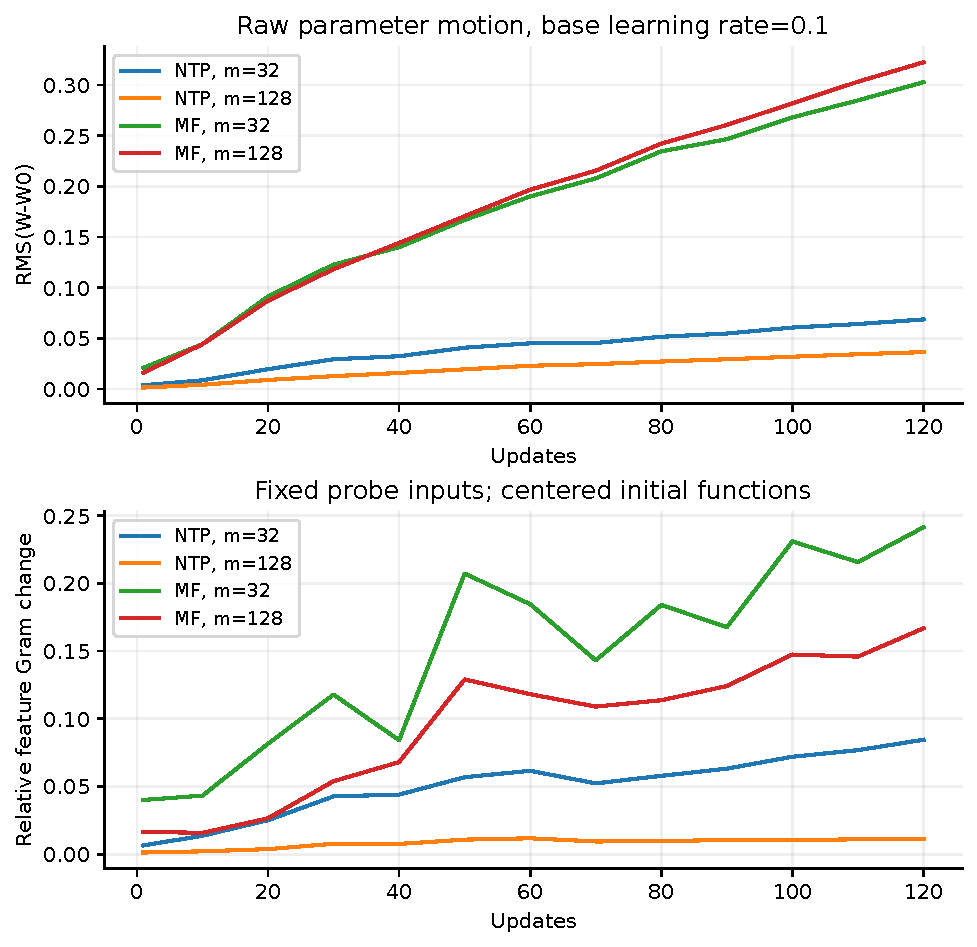
\includegraphics[width=0.85\textwidth]{figures/width_dynamics.pdf}
\caption{配套脚本的一次有限宽度运行：固定基础学习率、训练步数、batch 与探针输入，比较原始隐藏参数的移动和特征 Gram 漂移。两种参数化都减去冻结的初始函数；mean-field 使用原始参数步长 $m\eta$。这是一份单种子实验记录，图中的趋势需要通过多种子与更宽扫描检验，不能单独证明渐近尺度或性能优势。}
\label{l5:fig-width-dynamics}
\end{figure}

\section{隐式偏好、泛化与稳定性的收束}
\label{l5:closing}

\subsection{三件需要分别证明的事}

到这里，我们已经看到了三种不同层次的论断。
\begin{enumerate}
 \item \textbf{优化可达性：}给定参数化与算法，训练损失能否降低，速度与稳定范围如何？
 \item \textbf{隐式偏好：}若存在多个低损失或插值解，算法、初始化和步长倾向选择哪一类？
 \item \textbf{统计泛化：}这种被选择的解，在新的输入上是否与真实规律一致？
\end{enumerate}
最小范数结论回答第二个问题，但不单独回答第三个。因子分解的暂态谱偏好，首先描述训练路径，也不自动成为最终解的核范数定理。较大的特征漂移说明表示改变，不意味着泛化必然提升。一个完整的“适配数据”结论，应把数据或目标的结构假设加入推理链条。

\subsection{选读：局部平坦方向并不证明全局拓扑}

对平均平方损失，精确 Hessian 分解为
\begin{equation}
 \nabla_\theta^2L
 =\frac1nJ^\top J+
 \frac1n\sum_{i=1}^n r_i\nabla_\theta^2f_\theta(x_i).
 \label{l5:hessian-decomposition}
\end{equation}
在\emph{精确插值点}，残差项为零，因此 Hessian 半正定且秩至多为
$n$。若此处 $J$ 满行秩，隐函数定理进一步给出局部零损失集合是
$p-n$ 维流形，其切空间为 $\ker J$。如果只是接近插值，残差项小还需要二阶导有界，不能把近零特征值写成严格的零特征值。

这些都是局部陈述。参数个数大于样本数不单独保证整个零损失集合是一个连通流形，置换对称也不单独决定鞍点数量。关于更宽网络中某些对称极小值如何连接，已有在明确网络结构与嵌入假设下的研究\citep{Simsek2021}；本课程不把这些条件定理扩展成所有网络的拓扑定律。习题中的两神经元反例足以说明，两个等价极小值的中点甚至未必是驻点。

\subsection{Edge of Stability：对有限步长的观察}

对固定正定二次函数，普通 GD 的稳定条件为
\[
 0<\eta<\frac2{\lambda_{\max}(H)}.
\]
在一些神经网络全批量 GD 实验中，最大的 Hessian 特征值会在训练中变化，并在 $2/\eta$ 附近波动；损失在短期内可以非单调，而较长时间尺度继续降低。这类现象被称为 Edge of Stability，简称 EoS\citep{Cohen2021}。

这不违反固定 Hessian 二次目标的定理：非线性轨迹上的曲率在变，单个位置的二次近似也没有描述全部高阶动态。它提醒我们，有限步长训练可能超出单调下降和固定核近似的适用范围。

此外，$2/\eta$ 不是所有优化器共享的阈值。固定正定预条件 $P$ 下，二次模型的相关曲率是
$P^{1/2}HP^{1/2}$；带动量算法要分析含动量状态的迭代矩阵；Adam 和 Muon 还需要处理其自适应或谱变换状态。本课程的主宽度实验不以 EoS 是否出现作为成功标准，也不把原始 Hessian 变化单独当成特征学习的证据。

\subsection{选读：sharpness 与 SAM 的边界}

SAM 研究局部扰动下的目标
\begin{equation}
 \min_\theta\max_{\norm\delta_2\leq\rho}L(\theta+\delta)
 \label{l5:sam}
\end{equation}
及其可计算近似\citep{Foret2021}。在非驻点处，小半径展开首先包含
$\rho\norm{\nabla L(\theta)}_2$；在光滑驻点附近，二阶项才更直接地由 Hessian 的最大正曲率控制。因此 SAM 不能在所有位置都等同于给
$\lambda_{\max}(H)$ 加惩罚。

原始参数坐标中的 sharpness 还会随重参数化改变。某些保持网络函数不变的参数缩放，可以显著改变 Hessian 尺度，故不能无条件地用“更平坦”推出“泛化更好”\citep{Dinh2017}。这些边界并不削弱稳定性诊断的用途；它们说明解释诊断量时，必须同时说明坐标、优化器和比较协议。

\section{习题}
\label{l5:exercises}

\begin{exercise}[有效核与目标方向]
令 $F(\theta)=(\theta_1+\theta_2,\theta_1-\theta_2)^\top$，
$P=\diag(1,4)$，损失为 $\norm{F-y}_2^2/4$。
\begin{enumerate}
 \item 计算 $J$、$\mathcal K=JPJ^\top$ 与 $\Theta=\mathcal K/2$ 的特征值和特征向量。
 \item 给出普通预条件更新 $\theta^+=\theta-\eta P\nabla L$ 的稳定步长区间。
 \item 从零初始化，比较 $y=(1,1)^\top$ 与 $y=(1,-1)^\top$。取 $\eta=1/4$，分别计算一步后的残差。
 \item 找到线性坐标变换 $\theta=Su$，使对 $u$ 的欧氏 GD 与上述更新等价。
\end{enumerate}
\end{exercise}

\begin{exercise}[连续平衡与离散平衡]
设 $\ell(AB)=\norm{AB-Y}_F^2/2$，初值
$A=B=\diag(2,1)$，并取
\[
 Y=\begin{pmatrix}4&-1\\0&1\end{pmatrix}.
\]
\begin{enumerate}
 \item 计算初始梯度矩阵 $G=AB-Y$，验证初始化平衡。
 \item 用一次同时梯度更新计算 $A^+$ 与 $B^+$。
 \item 计算 $B^+(B^+)^\top-(A^+)^\top A^+$，判断离散 GD 是否精确保留平衡。
 \item 说明这一计算为何不反驳梯度流的平衡不变量。
\end{enumerate}
\end{exercise}

\begin{exercise}[宽度指数与输出坐标]
设两层模型的前向倍率为 $\kappa_m=m^{-s}$，原始 SGD 学习率为
$\eta m^t$。假设输入维度固定，初始化神经元的相关矩有界且非退化；对所讨论的有限训练区间，残差加权的单神经元梯度项保持典型 $O(1)$ 量级。
\begin{enumerate}
 \item 求有效核的典型量级及单神经元更新的典型量级。
 \item 若有效核要求保持非退化的 $\Theta(1)$ 量级，$s,t$ 应满足什么关系？若还要求单神经元更新不随宽度消失或发散，得到哪一组指数？
 \item 对 mean-field 模型令 $b=a/m$，重新推导实际输出权重的 SGD 步长。
 \item 在独立零均值输出初始化下，求原始初始输出方差关于 $m$ 的阶，并解释为什么实验需要控制初始函数。
\end{enumerate}
\end{exercise}

\begin{exercise}[对称极小值的中点反例]
考虑单样本 $x=1,y=5$，网络
\[
 f=v_1\operatorname{ReLU}(w_1x)+v_2\operatorname{ReLU}(w_2x),
 \qquad L=\frac12(f-y)^2.
\]
\begin{enumerate}
 \item 验证 $\theta=(w_1,v_1,w_2,v_2)=(1,1,2,2)$ 及其神经元交换
$\theta'=(2,2,1,1)$ 都是全局极小值。
 \item 计算中点处的预测、损失和完整梯度。
 \item 解释为什么交换对称性只强制某些反对称方向上的一阶导为零，不能推出中点是驻点。
 \item 说明该反例能够否定什么论断，以及它没有否定什么。
\end{enumerate}
\end{exercise}

\begin{exercise}[Hessian 变化是否说明特征学习]
考虑固定线性特征的单样本 logistic 模型：$F(w)=w$，正类标签下的损失
$L(w)=\log(1+e^{-w})$。
\begin{enumerate}
 \item 求预测 Jacobian $J$ 和损失 Hessian $L''(w)$。
 \item 计算 $w=0$ 与 $w\to+\infty$ 时的 Hessian，判断是否发生隐藏特征学习。
 \item 解释为什么不能仅凭训练中 Hessian 谱改变，就断言 NTK 固定核观点被反驳。
 \item 对平方损失写出式 \eqref{l5:hessian-decomposition}，说明把“近似插值”换成“精确插值”后，哪个结论从近似变成精确。
\end{enumerate}
\end{exercise}

\begin{exercise}[一份可复核的宽度迁移报告]
按第 \ref{l5:lab} 节的协议完成 NTP 与 mean-field SGD 比较。至少使用三个宽度、三个随机种子与一组共同基础学习率；训练步数和 batch 保持固定，默认中心化输出。
\begin{enumerate}
 \item 提交实际参数坐标与学习率表、原始初始输出 RMS、验证损失扫描、$D_W$ 和 $D_C$。
 \item 在查看结果之前定义“可迁移”的容忍阈值，并判断小宽度选出的学习率在较大宽度上是否满足该定义。
 \item 若 mean-field 越宽越慢，列出两个实现原因和一个模型或实验条件方面的原因，并说明如何分别核查。
 \item 若 NTP 在有限宽度下有明显特征漂移，写出一个有条件且不越界的结论。
 \item 可选做未配对 mean-field $+\eta$ 或冻结核参照，但必须说明它们各自检验的假设。
\end{enumerate}
\end{exercise}

\section{习题解答与核验要点}
\label{l5:solutions}

\subsection*{习题1：有效核与目标方向}

Jacobian 为
\[
 J=\begin{pmatrix}1&1\\1&-1\end{pmatrix},
 \qquad
 \mathcal K=\begin{pmatrix}5&-3\\-3&5\end{pmatrix},
 \qquad
 \Theta=\frac12\begin{pmatrix}5&-3\\-3&5\end{pmatrix}.
\]
沿 $q_+=(1,1)^\top/\sqrt2$ 的归一化特征值为 $1$，沿
$q_-=(1,-1)^\top/\sqrt2$ 的归一化特征值为 $4$，所以对任意初始残差都收敛的步长区间为 $0<\eta<1/2$。

第一种目标的残差 $r_0=(-1,-1)^\top$ 完全位于 $q_+$ 方向，取
$\eta=1/4$ 后变成 $r_1=(-3/4,-3/4)^\top$。第二种目标的残差
$r_0=(-1,1)^\top$ 位于 $q_-$ 方向，乘子 $1-\eta\lambda$ 等于零，一步后残差为零。相同模型、相同谱，目标投影不同便产生不同的有限步数表现。

取 $S=\diag(1,2)$，则 $SS^\top=P$。对 $u$ 作
$u^+=u-\eta S^\top\nabla_\theta L$，乘以 $S$ 后恰好得到
$\theta^+=\theta-\eta P\nabla_\theta L$。这是线性坐标下的精确等价，不涉及 Taylor 近似。

\subsection*{习题2：连续平衡与离散平衡}

初始乘积为 $AB=\diag(4,1)$，所以
\[
 G=\begin{pmatrix}0&1\\0&0\end{pmatrix},
 \qquad BB^\top=A^\top A=\diag(4,1).
\]
一次同时更新给出
\[
 A^+=\begin{pmatrix}2&-\eta\\0&1\end{pmatrix},
 \qquad
 B^+=\begin{pmatrix}2&-2\eta\\0&1\end{pmatrix}.
\]
注意第二个乘积是 $(A^+)^\top A^+$，不能在这里写成
$A^+(A^+)^\top$。直接相减得到
\[
 B^+(B^+)^\top-(A^+)^\top A^+
 =\begin{pmatrix}4\eta^2&0\\0&-\eta^2\end{pmatrix}.
\]
因此对任意非零步长都不再精确平衡。差值恰为二阶量，除以步长并令
$\eta\to0$ 后，一阶变化为零，与连续梯度流的不变量一致。若想由此获得长时间误差上界，还需要控制每一步矩阵的大小，不能只看单步的 $O(\eta^2)$。

\subsection*{习题3：宽度指数与输出坐标}

从式 \eqref{l5:two-layer-kernel} 可见，核中有 $m$ 项，每项前的系数为
$m^{t-2s}$，因此有效核的典型阶为
\[
 \mathcal K_m=O\!\left(m^{t+1-2s}\right).
\]
单神经元梯度含 $m^{-s}$，乘以学习率倍率后，更新为
$O(\eta m^{t-s})$。核保持非退化的 $O(1)$ 量级要求 $t=2s-1$；进一步要求单神经元更新既不消失也不增长，需 $t=s$。联立得到
$s=t=1$，即本讲的 mean-field 配对尺度。NTP 则是 $s=1/2,t=0$，其单神经元变化为 $O(\eta m^{-1/2})$。

对于 $b=a/m$，有 $g_a=g_b/m$，于是
\[
 \Delta b=\frac{\Delta a}{m}
 =-\frac{m\eta}{m}\,g_a
 =-\frac\eta m g_b.
\]
所以实际输出学习率为 $\eta/m$，而非 $m\eta$。

在独立零均值初始化下，原始输出方差为 $O(m^{1-2s})$，对应 RMS 为
$O(m^{1/2-s})$。NTP 的 RMS 为 $O(1)$，mean-field 为
$O(m^{-1/2})$。若不控制初始函数，比较会同时改变起点、参数化和更新尺度；默认中心化将起点固定为零，但仍应记录原始 RMS 检查初始化实现。

这些阶关系依赖题设中的典型非退化贡献。若数据、标签或参数处于特殊对称状态，某些梯度可以精确为零；量级分析不允许把这样的零量强行认作一般 $O(1)$ 信号。

\subsection*{习题4：对称极小值的中点反例}

两个端点的预测分别都是 $1\cdot1+2\cdot2=5$，损失为零，故均为全局极小值。中点四个参数都等于 $1.5$；由于隐藏输入为正，ReLU 在此可微。其预测为 $4.5$，残差为 $-0.5$，损失为 $0.125$。

对每个神经元，$\partial f/\partial w_r=v_r=1.5$、
$\partial f/\partial v_r=w_r=1.5$，所以
\[
 \nabla_\theta L=(-0.75,-0.75,-0.75,-0.75)^\top.
\]
中点不是驻点，更谈不上由 Hessian 分类的鞍点。

将两神经元写成平均部分与差分部分后，交换对称性使损失关于差分的联合符号翻转不变，故差分为零时的反对称一阶导为零。但平均部分的导数不必为零，端点的驻定条件也不会自动传给它们的平均。该反例否定的是“任意置换等价极小值的中点必为驻点或鞍点”的普遍说法。它没有否定置换等价性，也没有否定在额外条件下构造低损失连接路径或某些对称临界点的研究结果。

\subsection*{习题5：Hessian 变化与固定特征}

令 $s(w)=1/(1+e^{-w})$，则
\[
 J=1,\qquad L'(w)=s(w)-1,
 \qquad L''(w)=s(w)(1-s(w)).
\]
在 $w=0$ 时 Hessian 为 $1/4$，在 $w\to+\infty$ 时趋于零。模型的预测 Jacobian 一直为常数，没有任何隐藏特征可学习；变化来自损失对预测的曲率。因此，非平方损失下，即使 $JJ^\top$ 固定，参数损失 Hessian 仍可能变化。不能仅测 Hessian 就断言特征学习发生，也不能据此否定固定核的条件性理论。

平方损失的分解为
\[
 H=\frac1nJ^\top J+\frac1n\sum_i r_i\nabla^2f_i.
\]
在精确插值点，第二项严格为零，故 $H=J^\top J/n$、$H\succeq0$、
$\rank H\leq n$ 都是精确结论。在近似插值点，若二阶导有界，第二项才可被上界为一个小扰动；小扰动可以使原本的零特征值变成正或负的小数，不能继续声称 Hessian 严格低秩。

\subsection*{习题6：实验报告的判断方法}

这道题没有事先指定的一组数值曲线。可复核的答案首先应当确认三个配置层次：前向系数、实际存储变量和实际学习率相互一致；数据与训练预算固定；初始函数经过同样的中心化。漏掉任何一层，后续曲线都不能直接解释为宽度效应。

一个可接受的迁移定义可以是：在最小宽度上用验证集选出的基础学习率，在其他宽度均不发散，并且各自最终验证损失不超过该宽度扫描最优值加预先给定的容忍量。容忍量应在查看测试结果之前确定，且最好同时报告整个近最优区间，避免把极小的随机差异解释为迁移失败。

若 mean-field 越宽越慢，可先检查原始 $a,W$ 的步长是否错误地保持为
$\eta$，以及 forward 或 loss 是否重复除以宽度。第一项可通过打印参数组与一次手算更新核查，第二项可通过同一 batch 的手算损失和梯度尺度核查。若实现无误，还应检查基础步长是否过小、固定预算是否只覆盖了不同宽度的暂态，以及数据或初始化是否导致退化梯度；此时可以增加一个受控步长或训练时间对照，但不能在主扫描中悄悄改变预算。

若有限宽度 NTP 有明显特征漂移，合格结论应指出具体宽度、学习率和训练步数，并说“这一配置尚未接近固定特征近似”。还可以检查随宽度增大漂移是否减小，或与冻结核参照比较。不能直接推导“NTK 错误”，也不能反过来因理论预期而删去该实验。

未配对 mean-field 负对照主要检验前向与步长是否配平；冻结核参照主要检验固定 Jacobian 是否足以解释当前预测动态。前者不是统计泛化对照，后者也不能在随机 batch 协议不同的情况下独自定位特征学习来源。

\section{本讲概念检查}
\label{l5:checklist}

回到课程开头的问题：“从优化器角度，如何设计网络去适配数据？”本讲提供的回答步骤是：先写出实际参数化与更新，再得到数据上的有效几何；识别目标落在哪些方向，研究这些方向在初始化及训练过程中如何变化；最后通过固定预算的宽度扫描检验缩放与迁移。任何一步都需要可核验的假设或观测。

离开本讲前，应能独立解释以下区别：$JPJ^\top$ 与参数 Hessian、内部 Gram 平衡与左右输出 Gram、原始 $a$ 与实际输出 $b$、固定时间宽度极限与长时间训练、表示变化与泛化改善。能够说明这些区别，比记住一个没有坐标约定的“最佳学习率倍率”更有用。

\backmatter
\bibliographystyle{plainnat}
\bibliography{references}
\end{document}
